\section{计算极限值的若干方法}

计算极限值的方法有很多种, 常用的方法包括: 利用等价代换和初等变形、利用夹逼准则、利用 L'Hospital 法则以及利用 Taylor 展开等.

\subsection{利用等价代换和初等变形}

\subsubsection{等价代换}

% \begin{theorem}
%     若 $f\sim g$, 则 $f-g\sim f(\ln f-\ln g)$.
% \end{theorem}
% \begin{sol}
%     $\displaystyle f-g=\e ^{\ln f}-\e ^{\ln g}=\e ^\xi(\ln f-\ln g)\sim f(\ln f-\ln g)$, 
%     $\xi$ 介于 $\ln f$ 与 $\ln g$ 之间.
% \end{sol}

当 $x\to0$ 时, 下表是常见的等价代换.
\setcounter{magicrownumbers}{0}
\begin{table}[H]
    \centering
    \caption{常见的等价代换}
    \begin{tabular}{c l l l}
        \multirow{3}{*}{一阶} & \multicolumn{3}{l}{(\rownumber{}) $\displaystyle x\sim \sin x\sim \tan x\sim \arcsin x\sim \arctan x\sim \e ^x-1\sim \ln(1+x)$}                                                                                                                                                  \\
                              & (\rownumber{}) $\displaystyle \log_a(1+x)\sim\frac{x}{\ln a}$                                                                   & (\rownumber{}) $\displaystyle a^x-1\sim x\ln a$              & (\rownumber{}) $\displaystyle (1+x)^\alpha-1\sim \alpha x$                      \\
                              & (\rownumber{}) $\ln\qty(x+\sqrt{1+x^2})\sim x$                                                                                                                                                                                                                                   \\
        \midrule
        二阶                  & (\rownumber{}) $\displaystyle 1-\cos x\sim\frac{1}{2}x^2$                                                                       & (\rownumber{}) $\displaystyle x-\ln(1+x)\sim\frac{1}{2}x^2$  & (\rownumber{}) $\displaystyle (1+x)^x-1\sim x^2$                                \\
        \midrule
        \multirow{2}{*}{三阶} & (\rownumber{}) $\displaystyle x-\arctan x\sim\frac{1}{3}x^3$                                                                    & (\rownumber{}) $\displaystyle \tan x-x\sim\frac{1}{3}x^3$    & \multirow{2}{*}{(\rownumber{}) $\displaystyle \tan x-\sin x\sim\frac{1}{2}x^3$} \\
                              & (\rownumber{}) $\displaystyle x-\sin x\sim\frac{1}{6}x^3$                                                                       & (\rownumber{}) $\displaystyle \arcsin x-x\sim\frac{1}{6}x^3$ &                                                                                 \\
    \end{tabular}
\end{table}

\begin{figure}[H]
    \centering
    \begin{tikzpicture}[-,samples=100,>=stealth,scale=2,font=\footnotesize]
        \draw[->,cyan] (-3,0)--(3,0);
        \draw[fill=black] (-2,0)  circle(0.005) node[below] {$\arctan x$};
        \draw[fill=black] (-1,0)  circle(0.005) node[below] {$\sin x$};
        \draw[fill=black] (0,0)  circle(0.005) node[below] {$x$};
        \draw[fill=black] (1,0)  circle(0.005) node[below] {$\arcsin x$};
        \draw[fill=black] (2,0)  circle(0.005) node[below] {$\tan x$};
        \draw[decorate,decoration={brace,raise=3pt}] (-1,0) -- (0,0) node[midway,yshift=0.6cm] {$x-\sin x \sim \dfrac{1}{6}x^3$};
        \draw[decorate,decoration={brace,mirror,raise=10pt}] (-1,0) -- (2,0) node[midway,yshift=-0.8cm] {$\tan x-\sin x \sim \dfrac{3}{6}x^3$};
    \end{tikzpicture}
    \caption{}
\end{figure}

\begin{theorem}[差式无穷小代换]
    若 $f\sim g$, 则 $f-g\sim f(\ln f-\ln g)$.
    \label{fsimg}
    \index{差式无穷小代换}
\end{theorem}

\begin{example}[第一届数学竞赛初赛]
    设函数 $f(x),g(x)$ 在 $x=0$ 的某一邻域 $U$ 内有定义, 对 $\forall x\in U,~f(x)\neq g(x)$, 且 $\displaystyle\lim_{x\to0}f(x)=\lim_{x\to0}g(x)=a>0$, 求 $\displaystyle\lim_{x\to0}\dfrac{f^g-g^f}{f-g}.$
\end{example}
\begin{solution}
    由定理 \ref{fsimg} 可易求得该极限值为 $a^a.$
\end{solution}

\begin{example}
    求下列极限值.
    \label{liti 111}
    \setcounter{magicrownumbers}{0}
    \begin{table}[H]
        \centering
        \begin{tabular}{l | l | l}
            (\rownumber{}) $\displaystyle \lim_{x\to 0}\left(\frac{\sin x}{x}\right)^{\frac{1}{1-\cos x}}.$                                        & (\rownumber{}) $\displaystyle\lim_{x\to 0}\left(\frac{\arcsin x}{x}\right)^{\frac{1}{x^2}}.$                                                                         & (\rownumber{}) $\displaystyle \lim_{x\to\pi}\frac{\sin mx}{\sin nx}~ (m,n\in\mathbb{N}).$                    \\
            (\rownumber{}) $\displaystyle\lim _{x\to \pi /3}\dfrac{\tan ^{3}x-3\tan x}{\cos \left( x+\dfrac{\pi }{6}\right) }.$            & (\rownumber{}) $\displaystyle\lim _{x\to 0}\dfrac{\left( 1+x\right) ^{x}-\cos \dfrac{x}{2}}{\left( \sin x-\sin \dfrac{x}{2}\right) \ln \left( 1+x\right) }.$ & (\rownumber{}) $\displaystyle\lim _{x\to 0^{+}}\dfrac{x\ln \sin x-\sin x\ln x}{x^{3}\ln x}.$         \\
            (\rownumber{}) $\displaystyle \lim_{x\to1}\frac{1-\sqrt[n]{\cos 2n\pi x}}{(x-1)\left(x^x-1\right)}.$                                   & (\rownumber{}) $\displaystyle\lim_{n\to\infty}\frac{n^3\sqrt[n]{2}\left(1-\cos\dfrac{1}{n^2}\right)}{\sqrt{n^2+1}-n}$.                                               & (\rownumber{}) $\displaystyle\lim_{x\to-3}\frac{\left(x^2-9\right)\ln(4+x)}{\arctan^2(x+3)}.$                \\
            (\rownumber{}) $\displaystyle\lim_{x\to0}\frac{\displaystyle\prod\limits_{k=2}^{n}\left(1-\sqrt[k]{\cos x}\right)}{(1-\cos x)^{n-1}}.$ & (\rownumber{}) $\displaystyle\lim _{x\to 0}\dfrac{\displaystyle 1-\prod\limits ^{n}_{k=1}\sqrt[k] {\cos kx}}{x^{2}}.$                                        & (\rownumber{}) $\displaystyle\lim_{x\to0}\frac{\displaystyle n!x^n-\prod\limits_{k=1}^{n}\sin kx}{x^{n+2}}.$
        \end{tabular}
    \end{table}
\end{example}
\begin{solution}
    \begin{enumerate}[label=(\arabic*)]
        \item 原式= $\displaystyle\exp\lim_{x\to 0}\frac{1}{1-\cos x}\ln\frac{\sin x}{x}=\exp\lim_{x\to 0}\frac{1}{1-\cos x}\cdot \frac{\sin x-x}{x}=\exp\lim_{x\to 0}\frac{-\dfrac{1}{6}x^3}{\dfrac{1}{2}x^3}=\e ^{-\frac{1}{3}}$.
        \item 原式= $\displaystyle\exp\lim_{x\to 0}\frac{1}{x^2}\ln\frac{\arcsin x}{x}=\exp\lim_{x\to 0}\frac{1}{x^2}\cdot\frac{\arcsin x-x}{x}=\exp\lim_{x\to 0}\frac{\dfrac{1}{6}x^3}{x^3}=\e ^{\frac{1}{6}}$.
        \item $\displaystyle\text{原式}\xlongequal[]{t=x-\pi}\lim _{t\to 0}\dfrac{\sin m\left( t+\pi \right) }{\sin n\left( t+\pi \right) }=\lim _{t\to 0}\dfrac{\left( -1\right) ^{n}\sin mt}{\left( -1\right) ^{n}\sin nt}=\left( -1\right) ^{m-n}\dfrac{m}{n}.$
        \item $\displaystyle\text{原式}=\lim _{x\to \pi /3}\dfrac{\tan x\cdot \dfrac{\sin ^{2}x-3\cos ^{2}x}{\cos ^{2}x}}{\dfrac{\sqrt{3}}{2}\cos x-\dfrac{1}{2}\sin x}=\lim _{x\to \pi /3}\dfrac{\tan x\left( \sin x+\sqrt{3}\cos x\right) }{-\dfrac{1}{2}\cos x^{2}}=-24.$
        \item $\displaystyle\text{原式}=\lim _{x\to 0}\dfrac{\left( 1+x\right) ^{x}-1+\left( 1-\cos \dfrac{x}{2}\right) }{x\cdot \sin \dfrac{x}{2}\left( 2\cos \dfrac{x}{2}-1\right) }=\lim _{x\to 0}\dfrac{\left( 1+x\right) ^{x}-1}{\dfrac{x^{2}}{2}}+\lim _{x\to 0}\dfrac{1-\cos \dfrac{x}{2}}{\dfrac{x^{2}}{2}}=2+\dfrac{1}{4}=\dfrac{9}{4}.$
        \item $\displaystyle\text{原式}=\lim _{x\to 0^{+}}\dfrac{x\ln x-\sin x\ln x}{x^{3}\ln x}+\lim _{x\to 0^{+}}\dfrac{x\ln \sin x-x\ln x}{x^{3}\ln x}=\lim _{x\to 0^{+}}\dfrac{x-\sin x}{x^{3}}+\lim _{x\to 0^{+}}\dfrac{\ln \dfrac{\sin x}{x}}{x^{2}\ln x}=\dfrac{1}{6}.$
        \item 原式= $-\displaystyle\lim_{x\to1}\frac{\dfrac{1}{n}\ln\cos 2n\pi x}{(x-1)\ln x}\xlongequal[]{t=x-1}-\lim_{t\to0}\frac{\dfrac{1}{n}(\cos(2n\pi t)-1)}{t\ln(t+1)}=\lim_{t\to0}\frac{\dfrac{1}{n}\cdot\dfrac{1}{2}(2n\pi t)^2}{t^2}=2n\pi ^2.$
        \item 原式 $\displaystyle\xlongequal[]{\lim\limits_{n\to\infty}\sqrt[n]{2}=1}\lim_{n\to\infty}\frac{n^2\left(\dfrac{1}{2}\cdot\dfrac{1}{n^4}\right)}{\sqrt{1+\dfrac{1}{n^2}}-1}=\lim_{n\to\infty}\frac{\dfrac{1}{2n^2}}{\dfrac{1}{2n^2}}=1$.
        \item 原式= $\displaystyle\lim_{x\to-3}\frac{(x+3)(x-3)(x+3)}{(x+3)^2}=-6.$
        \item 由 $\displaystyle\lim_{x\to0}\frac{1}{\sqrt[k]{\cos x}}=1$, 即 $\displaystyle 1-\sqrt[k]{\cos x}\sim-\ln\sqrt[k]{\cos x}=-\frac{1}{k}\ln\cos x\sim\frac{1}{k}(1-\cos x)~ (x\to0)$,
              故 $$\text{原式}=\lim_{x\to0}\frac{\displaystyle\prod\limits_{k=2}^{n}\left[\dfrac{1}{k}(1-\cos x)\right]}{(1-\cos x)^{n-1}}=\frac{1}{n!}.$$
        \item 由 $\displaystyle\lim _{x\to 0}\dfrac{1}{\displaystyle\prod\limits ^{n}_{k=1}\sqrt[k] {\cos kx}}=1$, 故 $\displaystyle1-\prod ^{n}_{k=1}\sqrt[k] {\cos kx}\sim -\sum ^{n}_{k=1}\dfrac{1}{k}\ln \cos kx\sim \sum ^{n}_{k=1}\frac{1}{k}\ln \left( 1-\cos kx\right)(x\to0)$,
              \begin{flalign*}
                  \text{原式}=\lim _{x\to 0}\dfrac{\displaystyle\sum\limits ^{n}_{k=1}\dfrac{1}{k}\left( 1-\cos kx\right) }{x^{2}}=\sum ^{n}_{k=1}\lim _{x\to 0}\dfrac{\dfrac{1}{k}\cdot \dfrac{1}{2}\left( kx\right) ^{2}}{x^{2}}=\dfrac{1}{2}\sum ^{n}_{k=1}k=\dfrac{n\left( n+1\right) }{4}.
              \end{flalign*}
        \item \scriptsize\linespread{0.8}
              \textbf{法一: }因为 $\displaystyle\lim_{x\to0}\frac{n!x^n}{\displaystyle\prod\limits_{k=1}^{n}\sin kx}=1$, 所以 $\displaystyle n!x^n\sim\prod_{k=1}^{n}\sin kx~ (x\to0)$.
              \begin{flalign*}
                  \text{原式} & =\lim_{x\to0}\frac{\displaystyle n!x^n\left[\ln(n!x^n)-\ln\prod\limits_{k=1}^{n}\sin kx\right]}{x^{n+2}}=n!\lim_{x\to0}\frac{\displaystyle\sum\limits_{k=1}^{n}(\ln kx-\ln\sin kx)}{x^2}=n!\sum_{k=1}^{n}\lim_{x\to0}\frac{\ln\dfrac{kx}{\sin kx}}{x^2} \\
                              & =n!\sum_{k=1}^{n}\lim_{x\to0}\frac{\dfrac{kx}{\sin kx}-1}{x^2}=n!\sum_{k=1}^{n}\lim_{x\to0}\frac{kx-\sin kx}{kx^3}=\frac{n!}{6}\sum_{k=1}^{n}k^2=\frac{n(2n+1)}{36}(n+1)!.
              \end{flalign*}
              \textbf{法二: }原式= $\displaystyle n!\lim_{x\to0}\frac{1-\dfrac{\prod\limits_{k=1}^{n}\sin kx}{n!x^n}}{x^2}=n!\lim_{x\to0}\frac{\displaystyle 1-\prod\limits_{k=1}^{n}\dfrac{\sin kx}{kx}}{x^2}$, 记 $\displaystyle f_n(x)=\frac{\displaystyle 1-\prod\limits_{k=1}^{n}\dfrac{\sin kx}{kx}}{x^2}$, 则有
              \begin{flalign*}
                  f_n(x)=f_1(x)+\sum_{k=2}^{n}(f_k(x)-f_{k-1}(x))
              \end{flalign*}
              两边取极限有,
              \begin{flalign*}
                  \lim_{x\to0}f_n(x) & =\lim_{x\to0}f_1(x)+\lim_{x\to0}\sum_{k=2}^{n}(f_k(x)-f_{k-1}(x))=\frac{1}{6}+\lim_{x\to0}\sum_{k=2}^{n}\frac{\displaystyle\left(\prod\limits_{i=1}^{k-1}-\prod\limits_{i=1}^{k}\right)\dfrac{\sin ix}{ix}}{x^2} \\
                                     & =\frac{1}{6}+\lim_{x\to0}\frac{\displaystyle\prod\limits_{i=1}^{k-1}\dfrac{\sin ix}{ix}\left(1-\dfrac{\sin kx}{kx}\right)}{x^2}
                  =\frac{1}{6}+\lim_{x\to0}\sum_{k=2}^{n}\frac{kx-\sin kx}{kx^3}=\sum_{k=1}^{n}k^2=\frac{n(n+1)(2n+1)}{6}                                                                                                                               \\
                                     & \Rightarrow\text{原式}=\frac{n(2n+1)}{36}(n+1)!.
              \end{flalign*}
    \end{enumerate}
\end{solution}

\subsubsection{初等变形}

常见的裂项公式.
\setcounter{magicrownumbers}{0}
\begin{table}[H]
    \centering
    \caption{常见的裂项公式}
    \resizebox{.99\textwidth}{!}{
        \begin{tabular}{l l}
            (\rownumber{}) $\dfrac{1}{n(n+k)}=\dfrac{1}{k}\qty(\dfrac{1}{n}-\dfrac{1}{n+k})$       & (\rownumber{})  $\dfrac{1}{(n-k)n(n+k)}=\dfrac{1}{2k^2}\qty[\qty(\dfrac{1}{n-k}-\dfrac{1}{n})-\qty(\dfrac{1}{n}-\dfrac{1}{n+k})]$ \\
            \midrule
            (\rownumber{})  $\dfrac{1}{\sqrt{n+k}+\sqrt{n}}=\dfrac{1}{k}\qty(\sqrt{n+k}-\sqrt{n})$ & (\rownumber{})  $\dfrac{2^n}{\qty(2^n+k)\qty(2^{n+1}+k)}=\dfrac{1}{2^n+k}-\dfrac{1}{2^{n+1}+k}$
        \end{tabular}}
\end{table}

\begin{theorem}
    若 $B\sim \tilde{B}$, 且 $\exists a,~b$ 使得 $\lim A-\tilde{B}=a,~\lim \tilde{B}-B=b$, 则 $\lim A-B=a+b.$
\end{theorem}

\begin{example}
    求下列极限值.
    \setcounter{magicrownumbers}{0}
    \begin{table}[H]
        \centering
        \begin{tabular}{l | l | l}
            (\rownumber{}) $\displaystyle\lim_{n\to\infty}\prod_{k=2}^{n}\left(1-\frac{1}{k^2}\right).$ & (\rownumber{}) $\displaystyle \lim_{x\to0}\frac{1-\cos \sqrt{\tan x-\sin x}}{\sqrt[3]{1+x^3}-\sqrt[3]{1-x^3}}.$ & (\rownumber{}) $\displaystyle\lim_{n\to\infty}\cos^n\frac{x}{\sqrt{n}}.$                                  \\
            (\rownumber{}) $\displaystyle\lim_{n\to\infty}\sin^2\left(\pi\sqrt{n^2+n}\right).$          & (\rownumber{}) $\displaystyle\lim_{n\to \infty}\left(1+\sin \pi\sqrt{1+4n^2}\right)^n.$                         & (\rownumber{}) $\displaystyle\lim_{n\to\infty}\frac{2^{-n}}{n(n+1)}\sum_{k=1}^n \mathrm{C}_n^k\cdot k^2.$
        \end{tabular}
    \end{table}
\end{example}
\begin{solution}
    \begin{enumerate}[label=(\arabic{*})]
        \item $\displaystyle 1-\frac{1}{k^2}=\frac{(k-1)(k+1)}{k^2}$ 进行变形. $\displaystyle\text{原式}=\lim_{n\to\infty}\prod_{k=2}^{n}\frac{(k-1)(k+1)}{k^2}=\lim_{n\to\infty}\frac{n+1}{2n}=\frac{1}{2}.$
        \item 由 $\displaystyle\sqrt{\tan x-\sin x}=\sqrt{\frac{\sin x(1-\cos x)}{\cos x}}\sim\sqrt{\frac{x^3}{2}}$, 知 $\displaystyle 1-\cos\sqrt{\tan x-\sin x}\sim\frac{x^3}{4}$, \\
              又 $\displaystyle\sqrt[3]{1+x^3}-\sqrt[3]{1-x^3}=\frac{2x^3}{\left(\sqrt[3]{1+x^3}\right)^2+\sqrt[3]{1+x^3}\cdot\sqrt[3]{1-x^3}+\left(\sqrt[3]{1-x^3}\right)^2}\sim\frac{2x^3}{3}$,
              故原式= $\dfrac{3}{8}.$
        \item $\displaystyle\text{原式}=\lim_{n\to\infty}\left(1+\tan^2\frac{x}{\sqrt{n}}\right)^{-\frac{n}{2}}=\e ^{\lim\limits_{n\to\infty}\left(-\frac{n}{2}\right)\ln\left(1+\tan^2\frac{x}{\sqrt{n}}\right)}=\e ^{\lim\limits_{n\to\infty}\left(-\frac{n}{2}\right)\cdot\tan^2\frac{x}{\sqrt{n}}}=\e ^{-\frac{x^2}{2}}.$
        \item $\displaystyle\sin^2\left(\pi\sqrt{n^2+n}\right)=\sin^2\left(\pi\sqrt{n^2+n}-n\pi\right)=\sin^2\frac{n\pi}{\sqrt{n^2+n}+n}=\sin^2\frac{\pi}{\sqrt{1+\dfrac{1}{n}}+1}.$\\
              由于初等函数在有定义的地方皆连续, 故 $$\text{原极限}=\sin^2\left(\lim_{n\to\infty}\frac{\pi}{\sqrt{1+\dfrac{1}{n}}+1}\right)=\sin^2\frac{\pi}{2}=1.$$
        \item 由 $\displaystyle\sin\pi\sqrt{1+4n^2}=\sin\pi\left(\sqrt{1+4n^2}-2n\right)
                  =\sin\frac{\pi}{\sqrt{1+4n^2}+2n}.$
              \begin{flalign*}
                  \text{原式} & =\lim_{n\to\infty}\left(1+\sin\frac{\pi}{\sqrt{1+4n^2}+2n}\right)^n=\exp\lim_{n\to\infty}n\ln\left(1+\sin\frac{\pi}{\sqrt{1+4n^2}+2n}\right) \\
                              & =\exp\lim_{n\to\infty}\frac{n\pi}{\sqrt{1+4n^2}+2n}=\e ^{\frac{\pi}{4}}
              \end{flalign*}
        \item 因为 $\displaystyle(1+x)^n=\sum_{k=0}^n \mathrm{C}_n^k\cdot x^k$, 两边关于 $x$ 求导, 得 $\displaystyle n(1+x)^{n-1}=\sum_{k=1}^n \mathrm{C}_n^k\cdot kx^{k-1}$, 两边再同时乘以 $x$, 并再关于 $x$ 求导, 得
              $\displaystyle n(1+x)^{n-1}+n(n-1)x(1+x)^{n-2}=\sum_{k=1}^n \mathrm{C}_n^k\cdot k^2x^{k-1}$, 令 $x=1$, 得
              $$\displaystyle n\cdot 2^{n-1}+n(n+1)\cdot 2^{n-2}=n(n+1)\cdot 2^{n-2}=\sum_{k=1}^n \mathrm{C}_n^k k^2$$ 于是有原式
              $\displaystyle=\lim_{n\to\infty}\frac{2^{-n}}{n(n+1)}\cdot n(n+1)\cdot 2^{n-2}=\frac{1}{4}.$
    \end{enumerate}
\end{solution}

\begin{example}
    求 $\displaystyle\lim_{n\to\infty}x_n$, 设
    \setcounter{magicrownumbers}{0}
    \begin{table}[H]
        \centering
        \begin{tabular}{l | l}
            (\rownumber{}) $\displaystyle x_n=\cos\frac{x}{2}\cos\frac{x}{2^2}\cdots\cos\frac{x}{2^n}$. & (\rownumber{}) $\displaystyle x_n=\frac{3}{2}\frac{5}{4}\frac{17}{16}\cdots\frac{2^{2^n}+1}{2^{2^n}}$. \\
            (\rownumber{}) $\displaystyle x_n=\sum_{i=1}^n\frac{1}{\sqrt{1^3+2^3+\cdots+i^3}}$.         & (\rownumber{}) $\displaystyle x_n=\sum_{i=1}^n\frac{1}{i(i+1)(i+2)}$.                                  \\
            (\rownumber{}) $\displaystyle x_n=\sum_{k=1}^{n} \dfrac{k^3+6k^2+11k+5}{(k+3)!}$.
        \end{tabular}
    \end{table}
\end{example}
\begin{solution}
    \begin{enumerate}[label=(\arabic*)]
        \item 乘 $\displaystyle\frac{2^n\sin\dfrac{x}{2^n}}{2^n\sin\dfrac{x}{2^n}}$,
              $\displaystyle x_n=\cos\frac{x}{2}\cos\frac{x}{2^2}\cos\frac{x}{2^3}\cdots\cos\frac{x}{2^n}=\frac{2^n\sin\dfrac{x}{2^n}}{2^n\sin\dfrac{x}{2^n}}\cdot\prod_{k=1}^n\cos\frac{x}{2^k}=\frac{\sin x}{2^n\sin\dfrac{x}{2^n}}$
              \begin{flalign*}
                  \text{原式}=\lim_{n\to\infty}x_n=\lim_{n\to\infty}\frac{\sin x}{2^n\sin\dfrac{x}{2^n}}
                  =\lim_{n\to\infty}\frac{\sin x}{x}\cdot\frac{\dfrac{x}{2^n}}{\sin\dfrac{x}{2^n}}=\frac{\sin x}{x}.
              \end{flalign*}
        \item 乘 $\displaystyle\frac{1-\dfrac{1}{2}}{1-\dfrac{1}{2}}$, 再对分子反复应用公式 $(a+b)(a-b)=a^2-b^2.$
              $$x_n=\left(1+\frac{1}{2^{2^0}}\right)\left(1+\frac{1}{2^{2^1}}\right)\left(1+\frac{1}{2^{2^2}}\right)\cdots\left(1+\frac{1}{2^{2^n}}\right)=\dfrac{1-\dfrac{1}{2}}{1-\dfrac{1}{2}}\cdot\prod_{k=0}^n\left(1+\frac{1}{2^{2^k}}\right)\to 2~ (n\to\infty)$$
        \item 因为 $\displaystyle\sum_{i=1}^{n}i^3=\left(\sum_{i=1}^{n}i\right)^2$,
              \begin{flalign*}
                  \text{原式} & =\lim_{n\to\infty}\sum_{i=1}^n\frac{1}{\sqrt{\displaystyle\sum\limits_{j=1}^ij^3}}=\lim_{n\to\infty}\sum_{i=1}^n\frac{1}{\sqrt{\displaystyle\left(\sum\limits_{j=1}^ij\right)^2}}
                  =\lim_{n\to\infty}\sum_{i=1}^n\frac{1}{\dfrac{1}{2}i(i+1)}                                                                                                                                      \\
                              & =2\lim_{n\to\infty}\sum_{i=1}^n\left(\frac{1}{i}-\frac{1}{i+1}\right)=2\lim_{n\to\infty}\left(1-\frac{1}{n+1}\right)=2.
              \end{flalign*}
        \item $\displaystyle\lim_{n\to\infty}x_n=\frac{1}{2}\sum_{i=1}^n\left[\frac{1}{i(i+1)}-\frac{1}{(i+1)(i+2)}\right]=\frac{1}{2}\lim_{n\to\infty}\left[\frac{1}{2}-\frac{1}{(n+1)(n+2)}\right]=\frac{1}{4}.$
        \item 由于 $k^3+6k^2+11k+5=(k+1)(k+2)(k+3)-1$, 所以 $$
                  x_n=\sum_{k=1}^{n} \qty(\dfrac{1}{k!}-\dfrac{1}{(k+3)!})=\dfrac{1}{1!}+\dfrac{1}{2!}+\dfrac{1}{3!}-\dfrac{1}{(n+1)!}-\dfrac{1}{(n+2)!}-\dfrac{1}{(n+3)!}\to 1+\dfrac{1}{2}+\dfrac{1}{6}=\dfrac{5}{3}(n\to \infty)
              $$ 即 $\displaystyle \lim_{n \to \infty}x_n=\dfrac{5}{3}.$
    \end{enumerate}
\end{solution}

% \begin{example}
%     求极限 $\displaystyle I=\lim_{x\to0}\dfrac{\sqrt{\cos x}-\sqrt[3]{\cos x}}{x^3+\tan^2x}.$
% \end{example}
% \begin{solution}
%     由定理 \ref{fsimg}, 可得
%     \begin{flalign*}
%         I & =\lim_{x\to0}\dfrac{\sqrt{\cos x}\qty(\ln\sqrt{\cos x}-\ln\sqrt[3]{\cos x})}{x^3+\tan^2x}=\dfrac{1}{6}\lim_{x\to0}\dfrac{\ln\cos x}{x^3+\tan^2x}=\dfrac{1}{6}\lim_{x\to0}\dfrac{\cos x-1}{x^3+\tan^2x}=\dfrac{1}{6}\lim_{x\to0}\dfrac{\cos^2x\qty(\cos x-1)}{x^3\cos^2x+\sin^2x} \\
%           & =\dfrac{1}{6}\lim_{x\to0}\dfrac{\cos x-1}{x^3\cos^2x+\sin^2x}=-\dfrac{1}{3}\lim_{x\to0}\dfrac{\qty(\dfrac{\sin\frac{x}{2}}{\frac{x}{2}})^2\cdot x^2}{4\qty[x^2\qty(\dfrac{\sin x}{x})^2+x^3\cos^2x]}=-\dfrac{1}{3}\lim_{x\to0}\dfrac{1}{4x\cos^2x+4}=-\dfrac{1}{12}.
%     \end{flalign*}
% \end{solution}

\begin{example}
    求极限 $\displaystyle\lim_{n\to\infty}\dfrac{1}{n}\prod_{k=1}^{n}\dfrac{k+1-\sqrt{k^2+k}}{\sqrt{k}\qty(\sqrt{k+2}-\sqrt{k+1})}.$
\end{example}
\begin{solution}
    由 $\displaystyle\prod_{k=1}^{n}\dfrac{k+1-\sqrt{k^2+k}}{\sqrt{k}\qty(\sqrt{k+2}-\sqrt{k+1})}=\prod_{k=1}^{n}\dfrac{\sqrt{k+1}\qty(\sqrt{k+1}-\sqrt{k})}{\sqrt{k}\qty(\sqrt{k+2}-\sqrt{k+1})}=\prod_{k=1}^{n}\dfrac{\sqrt{k+1}}{\sqrt{k}}\cdot\prod_{k=1}^{n}\dfrac{\sqrt{k+1}-\sqrt{k}}{\sqrt{k+2}-\sqrt{k+1}}$, 因此
    \begin{flalign*}
        I & =\lim_{n\to\infty}\dfrac{1}{n}\prod_{k=1}^{n}\dfrac{\sqrt{k+1}}{\sqrt{k}}\cdot\prod_{k=1}^{n}\dfrac{\sqrt{k+1}-\sqrt{k}}{\sqrt{k+2}-\sqrt{k+1}}                                                                                                                                     \\
          & =\lim_{n\to\infty}\dfrac{1}{n}\dfrac{\sqrt{2}}{\sqrt{1}}\cdot\dfrac{\sqrt{3}}{\sqrt{2}}\cdots\dfrac{\sqrt{n+1}}{\sqrt{n}}\cdot\dfrac{\sqrt{2}-\sqrt{1}}{\sqrt{3}-\sqrt{2}}\cdot\dfrac{\sqrt{3}-\sqrt{2}}{\sqrt{4}-\sqrt{3}}\cdots\dfrac{\sqrt{n+1}-\sqrt{n}}{\sqrt{n+2}-\sqrt{n+1}} \\
          & =\lim_{n\to\infty}\dfrac{\sqrt{n+1}}{n}\cdot\dfrac{\sqrt{2}-\sqrt{1}}{\sqrt{n+2}-\sqrt{n+1}}=\qty(\sqrt{2}-1)\lim_{n\to\infty}\dfrac{\sqrt{n+1}\qty(\sqrt{n+2}+\sqrt{n+1})}{n}=2\sqrt{2}-2.
    \end{flalign*}
\end{solution}

\begin{example}
    设 \(\qty(1+\sqrt{3})^n=a_n+b_n\cdot\sqrt{3}\) (其中 \(a_n,b_n\) 均为正整数), 求 $\displaystyle\lim_{n\to\infty}\dfrac{a_n}{b_n}.$
\end{example}
\begin{solution}
    由二项式定理, $$\qty(1+\sqrt{3})^n=\sum_{k=0}^{n}\C_n^k\qty(\sqrt{3})^k=\sum_{\substack{2k\leqslant n\\k\in\mathbb{N}}}\C_n^k\qty(\sqrt{3})^k+\sum_{\substack{2k+1\leqslant n\\k\in\mathbb{N}}}\C_n^k\qty(\sqrt{3})^k=a_n+b_n\cdot\sqrt{3}$$
    则 $\qty(1-\sqrt{3})^n=a_n-b_n\cdot \sqrt{3}$, 联立两式解得
    $$\begin{cases}
            a_n=\dfrac{\qty(1+\sqrt{3})^n+\qty(1-\sqrt{3})^n}{2} \\[6pt]
            b_n=\dfrac{\qty(1+\sqrt{3})^n-\qty(1-\sqrt{3})^n}{2}
        \end{cases}$$
    则 $$\lim_{n\to\infty}\dfrac{a_n}{b_n}=\sqrt{3}\lim_{n\to\infty}\dfrac{\qty(1+\sqrt{3})^n+\qty(1-\sqrt{3})^n}{\qty(1+\sqrt{3})^n-\qty(1-\sqrt{3})^n}=\sqrt{3}.$$
\end{solution}

\subsection{利用已知极限}

\begin{example}[西安电子科技大学]
    求 $\displaystyle\lim_{n\to\infty}\left(\frac{\sqrt[n]{a}+\sqrt[n]{b}}{2}\right)^n~ (a,b\geqslant 0)$.
\end{example}
\begin{solution}
    \textbf{法一: }$\displaystyle n\left(\frac{\sqrt[n]{a}+\sqrt[n]{b}}{2}-1\right)=\frac{1}{2}\left(\frac{a^{\frac{1}{n}-1}}{\dfrac{1}{n}}+\frac{b^{\frac{1}{n}-1}}{\dfrac{1}{n}}\right)\to\frac{1}{2}(\ln a+\ln b)~ (n\to\infty)$,
    故 \begin{flalign*}
        \lim_{n\to\infty}\left(\frac{\sqrt[n]{a}+\sqrt[n]{b}}{2}\right)^n & =\lim_{n\to\infty}\left\{\left[1+\left(\frac{\sqrt[n]{a}+\sqrt[n]{b}}{2}-1\right)\right]^{\frac{1}{\frac{\sqrt[n]{a}+\sqrt[n]{b}}{2}-1}}\right\}^{n\left(\frac{\sqrt[n]{a}+\sqrt[n]{b}}{2}-1\right)} \\
                                                                          & =\e ^{\frac{1}{2}(\ln a+\ln b)}=\e ^{\ln\sqrt{ab}}=\sqrt{ab}.
    \end{flalign*}
    \textbf{法二: }$\displaystyle\text{原式}\xlongequal[]{x=\frac{1}{n}}\lim_{x\to0}\left(\frac{a^x+b^x}{2}\right)^{\frac{1}{x}}=\e ^{\lim\limits_{x\to0}\frac{1}{x}\ln\frac{a^x+b^x}{2}}=\e ^{\lim\limits_{x\to0}\frac{a^x\ln a+b^x\ln b}{a^x+b^x}}=\e ^{\frac{1}{2}(\ln a+\ln b)}=\sqrt{ab}.$
\end{solution}
\begin{inference}
    $\displaystyle a_i,p_i>0,i=1,2,\cdots,m,p=\sum_{i=1}^{m}p_i$, 则有
    $$\lim_{n\to\infty}\left(\frac{1}{m}\sum_{i=1}^{m}\sqrt[n]{a_i}\right)^n=\sqrt[m]{\prod_{i=1}^{m}a_i},~\lim_{n\to\infty}\left(\frac{1}{p}\sum_{i=1}^{m}p_i\cdot\sqrt[n]{a_i}\right)^n=\sqrt[p]{\prod_{i=1}^{m}a_i^{p_i}}.$$
\end{inference}
\begin{example}
    求下列极限值.
    \setcounter{magicrownumbers}{0}
    \begin{table}[H]
        \centering
        \begin{tabular}{l | l | l}
            (\rownumber{}) $\displaystyle\lim_{n\to\infty}\left(\frac{\sqrt[n]{2}+\sqrt[n]{3}+\sqrt[n]{5}}{3}\right)^n.$ & (\rownumber{}) $\displaystyle\lim_{n\to\infty}\left(\frac{2+\sqrt[n]{64}}{3}\right)^{2n-1}.$ & (\rownumber{}) $\displaystyle\lim_{x\to0}\left(\frac{a^{x+1}+b^{x+1}+c^{x+1}}{a+b+c}\right)^{\frac{1}{x}}.$
        \end{tabular}
    \end{table}
\end{example}
\begin{solution}
    \begin{enumerate}[label=(\arabic{*})]
        \item $\displaystyle\text{原式}=\sqrt[3]{2\times3\times5}=\sqrt[3]{30}.$
        \item \textbf{法一: }$\displaystyle\text{原式}\xlongequal[]{2n-1=t}\lim_{t\to\infty}\left(\frac{1+1+\sqrt[\frac{t+1}{2}]{64}}{3}\right)^t=\left(\sqrt[3]{64}\right)^2=16.$\\
              \textbf{法二: }$\displaystyle\text{原式}=\exp\lim_{x\to0}\left(\frac{2}{x}-1\right)\ln\left(\frac{2+64^x}{3}\right)=\exp\lim_{x\to0}\frac{(2-x)\left(64^x-1\right)}{3}\xlongequal[]{L'}\footnote{\text{该标记表示经 L'Hospital 法则得到的计算结果, 关于 L'Hospital 法则可见定理 }\ref{LHospitalLaw}.}\e ^{\frac{2}{3}\ln 64}=16.$
        \item $\displaystyle\text{原式}=\lim_{x\to0}\left(\frac{a\cdot a^x+b\cdot b^x+c\cdot c^x}{a+b+c}\right)^{\frac{1}{x}}=\sqrt[a+b+c]{a^ab^bc^c}.$
    \end{enumerate}
\end{solution}
\begin{example}
    求 $\displaystyle\lim_{n\to\infty}\left(\frac{1}{n+1}+\frac{1}{n+2}+\cdots+\frac{1}{2n}\right)$.
\end{example}

\begin{solution}
    为解决该问题, 先介绍并证明一个重要的等式,
    \begin{lemma}
        $\displaystyle x_n=1+\frac{1}{2}+\cdots+\frac{1}{n}-\ln n=\gamma+o(1)$, 其中 $\gamma=0.577215\cdots$ (称为 Euler 常数).
        \label{Euler C}
    \end{lemma}
    $\left| x_{n}-x_{n-1}\right| =\left| \dfrac{1}{n}-\left[ \ln n-\ln \left( n-1\right) \right] \right| ,n\geqslant 2$
    由 Lagrange 中值定理 $$\ln n-\ln(n-1)=\dfrac{1}{\xi_n}~ (n-1<\xi_n<n)$$
    $\left| x_{n}-x_{n-1}\right| =\dfrac{n-\xi _{n}}{n\cdot \xi _{n}} <\dfrac{1}{\left( n-1\right) ^{2}}$,
    而 $\displaystyle\sum_{n=2}^{\infty}\dfrac{1}{(n-1)^2}$ 收敛, 故 $\displaystyle\sum_{n=2}^{\infty}|x_n-x_{n-1}|$ 收敛, $x_n$ 也收敛.
    \begin{flalign*}
        \text{原式}  =\lim_{n\to\infty}\left(\sum_{i=1}^{2n}\frac{1}{i}-\sum_{i=1}^n\frac{1}{i}\right)
        =\lim_{n\to\infty}\left[\left(\ln 2n +\gamma+\alpha_{2n}\right)-\left(\ln n+\gamma +\alpha_n\right)\right]
        =\lim_{n\to\infty}\left(\ln 2+\alpha_{2n}-\alpha_{n}\right)=\ln 2
    \end{flalign*}
    其中 $\gamma$ 为 Euler 常数.
\end{solution}
\begin{inference}
    已知 $m$ 为正整数, 则有 $$\lim_{n\to\infty}\left[\frac{1}{mn+1}+\frac{1}{mn+2}+\cdots+\frac{1}{(m+1)n}\right]=\ln\frac{m+1}{m}.$$
\end{inference}
\begin{proof}[{\songti \textbf{证}}]
    $\displaystyle\lim_{n\to\infty}\sum_{k=1}^{n}\frac{1}{mn+k}=\lim_{n\to\infty}\frac{1}{n}\sum_{k=1}^{n}\frac{1}{m+\dfrac{k}{n}}=\int_{0}^{1}\frac{\dd x}{m+x}=\ln\frac{m+1}{m}.$
\end{proof}
\begin{example}
    \scriptsize\linespread{0.8}
    试借助 Stirling 公式 $$n!=\sqrt{2\pi n}n^n\e ^{-n+\frac{\theta_n}{12n}},~0\leqslant \theta_n\leqslant 1$$
    求极限 $\displaystyle \lim_{n\to\infty}\sqrt{n}\prod_{i=1}^n\frac{\e ^{1-\frac{1}{i}}}{\left(1+\frac{1}{i}\right)^i}$.
    \label{Stirling}
\end{example}
\begin{solution}
    \scriptsize\linespread{0.8}
    由引理 \ref{Euler C}, 得
    \begin{flalign*}
        \text{原式} & =\lim_{n\to\infty}\sqrt{n}\frac{\e ^{n-\sum\limits_{i=1}^n\frac{1}{i}}}{\displaystyle\prod\limits_{i=1}^n\left(\dfrac{i+1}{i}\right)^i}
        =\lim_{n\to\infty}\frac{\sqrt{n}\cdot n!\e ^{n-\sum\limits_{i=1}^n\frac{1}{i}}}{(n+1)^n}
        =\lim_{n\to\infty}\frac{\sqrt{n}\sqrt{2\pi n}\cdot n^n\e ^{\frac{\theta_n}{12n}}}{(n+1)^n\e ^{\sum\limits_{i=1}^n\frac{1}{i}}}                        \\
                    & =\lim_{n\to\infty}\frac{\sqrt{2\pi}n\e ^{\frac{\theta_n}{12n}}}{\left(1+\dfrac{1}{n}\right)^n\e ^{\sum\limits_{i=1}^n\frac{1}{i}}}
        =\sqrt{2\pi}\exp\lim_{n\to\infty}\left(\ln n+\frac{\theta_n}{12n}-\sum_{i=1}^n\frac{1}{i}\right)
        =\sqrt{2\pi}\e ^{-(1+\gamma)}
    \end{flalign*}
    其中 $\gamma$ 为 Euler 常数.
\end{solution}

\subsection{利用函数与极限的关系}

\begin{theorem}[极限值与函数式的转换]
    $\lim f(x)=A\Leftrightarrow f(x)=A+\alpha(x),~\alpha(x)\to0.$
    \index{极限值与函数式的转换}
\end{theorem}

\begin{theorem}[分式极限的关系]
    设 $\displaystyle\lim\frac{f(x)}{g(x)}=A$, $A$ 为有限常数, 则
    \label{f(x)g(x)A}
    \begin{enumerate}[label=(\arabic{*})]
        \item 当 $g(x)\to0$ 时, 必有 $f(x)\to0$;
        \item 当 $f(x)\to0$, 且 $A\not=0$ 时, 必有 $g(x)\to0$.
    \end{enumerate}
    \index{分式极限的关系}
\end{theorem}

\begin{example}
    设函数 $f(x)$ 在 $x=0$ 的某个邻域内有连续导数, 且 $\displaystyle\lim_{x\to0}\left(\frac{\sin x}{x^2}+\frac{f(x)}{x}\right)=2$, 求 $f(0)'.$
\end{example}
\begin{solution}
    由已知 $\displaystyle\lim_{x\to0}\left(\frac{\sin x}{x^2}+\frac{f(x)}{x}\right)=2$, 得
    $\displaystyle f(x)=2x-\frac{\sin x}{x}+x\cdot\alpha(x),~\alpha(x)\to0~ (x\to0)$,
    则有 $$f(0)=\lim_{x\to0}f(x)=\lim_{x\to0}\left(2x-\frac{\sin x}{x}+x\cdot \alpha(x)\right)=-1$$
    $$f(0)'=\lim_{x\to0}\frac{f(x)-f(0)}{x}=\lim_{x\to0}\frac{f(x)+1}{x}=\lim_{x\to0}\left(2+\frac{x-\sin x}{x^2}+\alpha(x)\right)=2.$$
\end{solution}
\begin{example}
    (运用两种方法) 根据假设求极限.
    \setcounter{magicrownumbers}{0}
    \begin{table}[H]
        \centering
        \begin{tabular}{l | l}
            (\rownumber{}) $\displaystyle\lim_{x\to0}\frac{\sin 6x+xf(x)}{x^3}=0$, $\displaystyle\lim_{x\to0}\frac{6+f(x)}{x^2}.$                           & (\rownumber{}) $\displaystyle\lim_{x\to0}\frac{\ln(1+2x)+xf(x)}{\sin x^2}=2$, $\displaystyle\lim_{x\to0}\frac{2+f(x)}{x}.$                                    \\
            (\rownumber{}) $\displaystyle\lim_{x\to0}\frac{\ln\left(1+\dfrac{f(x)}{\sin 2x}\right)}{3^x-1}=5$, $\displaystyle\lim_{x\to0}\frac{f(x)}{x^2}.$ & (\rownumber{}) $\displaystyle\lim_{x\to0}\frac{\ln\left(1+\dfrac{3f(x)}{1-\cos x}\right)}{\e ^x-1}=9$, $\displaystyle\lim_{x\to0}\frac{f(x)}{\tan x-\sin x}.$
        \end{tabular}
    \end{table}
\end{example}
\begin{solution}
    \begin{enumerate}[label=(\arabic{*})]
        \item \textbf{法一 :}由已知得 $\displaystyle f(x)=\frac{-\sin 6x+x^3\cdot\alpha(x)}{x},~\alpha(x)\to0$, 故
              $$\lim_{x\to0}\frac{6+f(x)}{x^2}=\lim_{x\to0}\frac{6x-\sin 6x+x^3\cdot\alpha(x)}{x^3}=\frac{\dfrac{1}{6}(6x)^3}{x^3}=36.$$
              \textbf{法二: }$\displaystyle\lim_{x\to0}\frac{6+f(x)}{x^2}=\lim_{x\to0}\frac{6x+xf(x)}{x^3}=\lim_{x\to0}\left(\frac{\sin 6x+xf(x)}{x^3}+\frac{6x-\sin 6x}{x^3}\right)=36.$
        \item \textbf{法一: }由已知得 $\displaystyle f(x)=\frac{2\sin x^2+\alpha(x)\cdot \sin x^2-\ln(1+2x)}{x}$, $\alpha(x)\to0$, 故
              \begin{flalign*}
                  \lim_{x\to0}\frac{2+f(x)}{x}  =\lim_{x\to0}\frac{2x+2\sin x^2+\alpha(x)\sin x^2-\ln(1+2x)}{x^2}
                  =\lim_{x\to0}\left[\frac{2\sin x^2}{x^2}+\frac{2x-\ln(1+2x)}{x^2}\right]=4.
              \end{flalign*}
              \textbf{法二: }因为 $x\sim\sin x~ (x\to0)$, 所以 $\displaystyle\frac{2+f(x)}{x}=\frac{2x+xf(x)}{x^2}\sim\frac{2x+f(x)}{\sin x^2}$, 故
              $$\lim_{x\to0}\frac{2+f(x)}{x}=\lim_{x\to0}\left[\frac{\ln(1+2x)+xf(x)}{\sin x^2}+\frac{2x-\ln(1+2x)}{x^2}\right]=2+2=4.$$
        \item \textbf{法一: }由已知得 $\displaystyle f(x)=\sin2x\cdot\left[\e ^{(5+\alpha(x))\cdot(3^x-1)}-1\right],~\alpha(x)\to0$, 故
              $$\lim_{x\to0}\frac{f(x)}{x^2}=\lim_{x\to0}\frac{\sin2x\cdot(5+\alpha(x))\cdot(3^x-1)}{x^2}=\lim_{x\to0}\frac{2x\cdot(5+\alpha(x))\cdot x\ln3}{x^2}=10\ln3.$$
              \textbf{法二: }因为 $\displaystyle\lim_{x\to0}(3^x-1)=0$, 所以有 $\displaystyle\lim_{x\to0}\ln\left(1+\frac{f(x)}{\sin2x}\right)=\lim_{x\to0}\frac{\ln\left(1+\dfrac{f(x)}{\sin2x}\right)}{3^x-1}\cdot(3^x-1)=0.$\\
              于是 $\displaystyle\lim_{x\to0}\frac{f(x)}{\sin2x}=0$, 从而当 $x\to0$ 时, $\displaystyle\ln\left(1+\frac{f(x)}{\sin2x}\right)\sim\frac{f(x)}{\sin2x}$.
              又 $3^x-1\sim x\ln3,~x\to0$, 再由已知
              $$5=\lim_{x\to0}\frac{\ln\left(1+\dfrac{f(x)}{\sin2x}\right)}{3^x-1}=\lim_{x\to0}\frac{\dfrac{f(x)}{\sin2x}}{x\cdot\ln3}=\lim_{x\to0}\frac{f(x)}{2\ln3\cdot x^2}$$
              故得 $\displaystyle\lim_{x\to0}\frac{f(x)}{x^2}=10\ln3.$
        \item \textbf{法一: }由已知得 $\displaystyle f(x)=\left[\e ^{(9+\alpha(x))(\e ^x-1)}-1\right]\cdot\frac{1-\cos x}{3}\sim(9+\alpha(x))\cdot\frac{1}{3}\cdot\frac{1}{2}\cdot x^3,~\alpha(x)\to0$, \\
              且 $\displaystyle\tan x-\sin x\sim\frac{1}{2}x^3,~x\to0$, 所以 $\displaystyle\lim_{x\to0}\frac{x}{\tan x-\sin x}=3.$\\
              \textbf{法二: }同上例解法 2.
    \end{enumerate}
\end{solution}

\subsection{利用夹逼准则}

当极限不易直接求出时, 可考虑将求极限的变量, 作适当的放大和缩小, 使放大、缩小所得的新变量易于求极限,
且二者的极限值相同, 则原极限存在, 且等于公共值.

% \begin{theorem}[夹逼准则的函数形式]
%     设函数 $g(x)\leqslant f(x)\leqslant h(x)$, 如果在自变量 $x$ 的同一变化过程中, 则
%     $$\lim g(x)=\lim h(x)=A\Rightarrow \lim f(x)=A$$
%     定理 \ref{pinchGuidelines} 给出了数列形式的情况.
%     \index{夹逼准则的函数形式}
% \end{theorem}

\begin{example}
    证明 $\displaystyle\lim_{n\to\infty}\sqrt[n]{n}=1.$ (该结论可作为重要极限使用).
    \label{sqrtnn1}
\end{example}
\begin{proof}[{\songti \textbf{证法一}}]
    因为 $\displaystyle(a+b)^n=\sum_{k=0}^{n}\mathrm{C}_n^ka^kb^{n-k}$, 所以当 $n\leqslant 2$ 时, 由
    $$n=1+(n-1)=1+\frac{n(n-1)}{2}\cdot\frac{2}{n}=1+\mathrm{C}_n^2\left(\sqrt{\frac{2}{n}}\right)^2<\left(1+\sqrt{\frac{2}{n}}\right)^n$$
    得 $\displaystyle 1<\sqrt[n]{n}<\sqrt{\frac{2}{n}}$, 于是由夹逼准则得 $\displaystyle\lim_{n\to\infty}\sqrt[n]{n}=1.$
\end{proof}
\begin{proof}[{\songti \textbf{证法二}}]
    由定理 \ref{meanInequality} 知算术-几何-调和平均值不等式: 设 $a_i>0~ (i=1,2,\cdots,n)$, 则有
    $$\frac{n}{\displaystyle\sum_{i=1}^{n}\dfrac{1}{a_i}}\leqslant\sqrt[n]{\prod_{i=1}^{n}a_i}\leqslant \frac{1}{n}\sum_{i=1}^{n}a_i$$
    因为 $n$ 可看作两个 $\sqrt{n}$ 与 $n-2$ 个 $1$ 的乘积, 所以由上述不等式有
    $$\frac{2}{\dfrac{2}{\sqrt{n}}+n-2}\leqslant\sqrt[n]{n}=\sqrt[n]{\sqrt{n}\cdot\sqrt{n}\cdot\underbrace{1\cdot1\cdots1}_{n-2}}\leqslant\frac{2\sqrt{n}+n-2}{n}<1+\frac{2}{\sqrt{n}}$$
    而 $\displaystyle\lim_{n\to\infty}\frac{n}{\dfrac{2}{\sqrt{n}}+n-2}=1,~\lim_{n\to\infty}\left(1+\frac{2}{\sqrt{n}}\right)=1$, 故由夹逼准则得 $\displaystyle\lim_{n\to\infty}\sqrt[n]{n}=1.$
\end{proof}

\begin{example}
    (要求用夹逼准则求解) 求极限 $\displaystyle\lim_{n\to\infty}x_n$, 设
    \setcounter{magicrownumbers}{0}
    \begin{table}[H]
        \centering
        \begin{tabular}{l | l}
            (\rownumber{}) (东北师范大学) $\displaystyle x_n=\frac{1\cdot3\cdots(2n-1)}{2\cdot4\cdots(2n)}.$                                   & (\rownumber{}) $\displaystyle x_n=\sum_{k=n^2}^{(n+1)^2}\frac{1}{\sqrt{k}}.$ \\
            (\rownumber{}) $\displaystyle x_n=\sum_{k=1}^{n}\left[\left(n^k+1\right)^{-\frac{1}{k}}+\left(n^k-1\right)^{-\frac{1}{k}}\right].$ & (\rownumber{}) (北京大学) $\displaystyle x_n=(n!)^{\frac{1}{n^2}}.$          \\
            (\rownumber{}) $\displaystyle x_n=\frac{1}{n+1}+\frac{1}{n+2}+\cdots+\frac{1}{n+n}.$                                               & (\rownumber{}) (中国地质大学) $\displaystyle x_n=\frac{\sqrt[n]{n!}}{n}.$    \\
            (\rownumber{}) (2003 浙江省数学竞赛) $\displaystyle x_n=\sum_{k=1}^{n}\frac{n+k}{n^2+k}.$                                          & (\rownumber{}) $\displaystyle x_n=\sqrt[n]{\sum_{k=1}^{m}a_k^n},~a_k>0.$
        \end{tabular}
    \end{table}
\end{example}
\begin{solution}
    \begin{enumerate}[label=(\arabic{*})]
        \item 因为几何平均小于算术平均, 故分母中的因子
              $$2n=\frac{(2n-1)+(2n+1)}{2}>\sqrt{(2n-1)(2n+1)}$$
              由此可知 $$0<x_n=\frac{1\cdot3\cdots(2n-1)}{2\cdot4\cdots(2n)}<\frac{1}{\sqrt{2n+1}}\to0$$
              故 $\displaystyle\lim_{n\to\infty}x_n=0.$
        \item $\displaystyle\sum_{k=n^2}^{(n+1)^2}\frac{1}{\sqrt{k}}$ 共有 $2n+2$ 项, 最小项为 $\displaystyle\frac{1}{\sqrt{(n+1)^2}}=\frac{1}{n+1}$,
              最大项为 $\displaystyle\frac{1}{n}$, 因此
              $$\frac{2n+2}{n+1}\leqslant\sum_{k=n^2}^{(n+1)^2}\frac{1}{\sqrt{k}}\leqslant\frac{2n+2}{n}$$
              左右两端极限均为 $2$, 故 $\displaystyle\lim_{n\to\infty}\sum_{k=n^2}^{(n+1)^2}\frac{1}{\sqrt{k}}=2.$
        \item 因为 $n^k<n^k+1<(n+1)^k$, 所以
              $$n^{-1}(n^k+1)^{-\frac{1}{k}}>(n+1)^{-1}~ (k=1,2,\cdots,n)$$
              相加得 $\displaystyle\frac{n}{n}>\sum_{k=1}^{n}(n^k+1)^{-\frac{1}{k}}>\frac{n}{n+1}$.
              令 $n\to\infty$, 取极限得 $\displaystyle\lim_{n\to\infty}\sum_{k=1}^{n}(n^k+1)^{-\frac{1}{k}}=1$.\\
              同理可得 $\displaystyle\lim_{n\to\infty}\sum_{k=1}^{n}(n^k-1)^{-\frac{1}{k}}=1$, 从而 $\displaystyle\lim_{n\to\infty}x_n=2.$
        \item $\displaystyle 1\leqslant (n!)^{\frac{1}{n^2}}\leqslant (n^n)^{\frac{1}{n^2}}=n^{\frac{1}{n}}$, 因为 $\displaystyle\lim_{n\to\infty}\sqrt[n]{n}=1$ (见例 \ref{sqrtnn1}),
              所以 $\displaystyle\lim_{n\to\infty}(n!)^{\frac{1}{n^2}}=1.$
        \item 由对数不等式 $$\frac{1}{n+1}\leqslant\ln\left(1+\frac{1}{n}\right)\leqslant\frac{1}{n}$$
              $$\ln\left(1+\frac{1}{n+1}\right)+\cdots+\ln\left(1+\frac{1}{n+n}\right)\leqslant x_n\leqslant \ln\left(1+\frac{1}{n}\right)+\cdots+\ln\left(1+\frac{1}{n+n-1}\right)$$
              $\displaystyle\text{左端}=\ln\left(\frac{n+2}{n+1}\cdot\frac{n+3}{n+2}\cdots\frac{n+n}{n+n-1}\cdot\frac{n+n+1}{n+n}\right)=\ln\frac{2n+1}{n+1}\to\ln2~ (n\to\infty)$.\\
              同理, 右端$=\displaystyle\ln\frac{2n}{n}\to\ln2~ (n\to\infty)$, 所以 $\displaystyle\lim_{n\to\infty}x_n=\ln 2.$
        \item 利用不等式: $\displaystyle\left(\frac{n+1}{\e }\right)^n< n!<\e \left(\frac{n+1}{\e }\right)^{n+1}$, 知
              $$\frac{1}{\e }\cdot\frac{n+1}{n}<\frac{\sqrt[n]{n!}}{n}<\sqrt[n]{\e }\cdot\frac{1}{\e }\cdot\frac{n+1}{n}\cdot\sqrt[n]{\frac{n+1}{\e }}$$
              故有夹逼准则, 得 $\displaystyle\lim_{n\to\infty}\frac{\sqrt[n]{n!}}{n}=\frac{1}{\e }.$
        \item 因为 $\displaystyle\frac{n+k}{n^2+n}\leqslant\frac{n+k}{n^2+k}<\frac{n+k}{n^2},~k=1,2,\cdots,n$, 所以
              $$\sum_{k=1}^{n}\frac{n+k}{n^2+n}\leqslant\sum_{k=1}^{n}\frac{n+k}{n^2+k}<\sum_{k=1}^{n}\frac{n+k}{n^2}$$
              $$\lim_{n\to\infty}\sum_{k=1}^{n}\frac{n+k}{n^2+n}=\lim_{n\to\infty}\frac{1}{n^2+n}\sum_{k=1}^{n}(n+k)=\lim_{n\to\infty}\frac{3n^2+n}{2n^2+2n}=\frac{3}{2}$$
              $$\lim_{n\to\infty}\sum_{k=1}^{n}\frac{n+k}{n^2}=\lim_{n\to\infty}\frac{1}{n^2}\sum_{k=1}^{n}(n+k)=\lim_{n\to\infty}\frac{3n^2+n}{2n^2}=\frac{3}{2}$$
              故由夹逼准则, 得 $\displaystyle\lim_{n\to\infty}\sum_{k=1}^{n}\frac{n+k}{n^2+k}=\frac{3}{2}.$
        \item 记 $\displaystyle a_{i0}=\max_{1\leqslant j\leqslant m}\{a_j\}$, 则 $\displaystyle a_{i0}<\sum_{k=1}^{m}a_k^n<m a_{i0}^n$, 于是 $\displaystyle a_{i0}<\sqrt[n]{\sum_{k=1}^{m}a_k^n}<\sqrt[n]{m}a_{i0}$,
              由 $\displaystyle\lim_{n\to\infty}\sqrt[n]{m}=1$ 及夹逼准则得 $\displaystyle\lim_{n\to\infty}\sqrt[n]{\sum_{k=1}^{m}a_k^n}=a_{i0}=\max\{a_1,a_2,\cdots,a_m\}.$
    \end{enumerate}
\end{solution}
\begin{inference}
    设 $\displaystyle a_i,p_i>0,~i=1,2,\cdots,m,~p=\sum_{i=1}^{m}p_i$, 则有
    $$\displaystyle\lim_{n\to\infty}\sqrt[n]{\frac{1}{m}\sum_{i=1}^{m}a_i^n}=\displaystyle \lim_{n\to\infty}\sqrt[n]{\frac{1}{p}\sum_{i=1}^{m}p_ia_i^n}=\displaystyle \lim_{n\to\infty}\sqrt[n]{\sum_{i=1}^{m}p_ia_i^n}=\displaystyle \lim_{x\to+\infty}\sqrt[x]{\sum_{i=1}^{m}p_ia_i^x}=\max_{1\leqslant i\leqslant m}\{a_i\}.$$
    \label{maxai}
\end{inference}
\begin{example}
    求下列极限值.
    \setcounter{magicrownumbers}{0}
    \begin{table}[H]
        \centering
        \begin{tabular}{l | l | l}
            (\rownumber{}) $\displaystyle\lim_{n\to\infty}\sqrt[n]{1+2^n\cdot\sin^nx}.$ & (\rownumber{}) $\displaystyle\lim_{n\to\infty}\sqrt[n]{\sin^2n+2\cos^2n}.$ & (\rownumber{}) $\displaystyle\lim_{n\to\infty}\sqrt[n]{2^n+a^{2n}}$, $a$ 为常数.
        \end{tabular}
    \end{table}
\end{example}
\begin{solution}
    \begin{enumerate}[label=(\arabic{*})]
        \item $\displaystyle\text{原式}=\max\{1,2\sin x\}=\begin{cases}
                      2\sin x       & ,|\sin x|>\dfrac{1}{2}                      \\
                      1             & ,-\dfrac{1}{2}<\sin x\leqslant \dfrac{1}{2} \\
                      \text{不存在} & ,\sin x=-\dfrac{1}{2} .
                  \end{cases}$
        \item $\displaystyle\text{原式}=\lim_{n\to\infty}\sqrt[n]{1+\left(\cos^{\frac{2}{n}}n \right)^n}=\max\left\{1,\cos^{\frac{2}{n}}n\right\}=1.$,
              其中易求得 $\displaystyle \cos^{\frac{2}{n}}n$ 的最大值为 1.
        \item $\displaystyle\text{原式}=\lim_{n\to\infty}\sqrt[n]{2^n+\underbrace{a^n+a^n+\cdots+a^n}_{a_n}}=\max\{2,a\}.$
    \end{enumerate}
\end{solution}

\begin{example}
    求极限 $\displaystyle\lim_{n\to\infty}\qty(\dfrac{n}{3}-\sum_{k=1}^{n}\dfrac{k^2}{n^2+k}).$
\end{example}
\begin{solution}
    因为 $\displaystyle\dfrac{n}{3}-\sum_{k=1}^{n}\dfrac{k^2}{n^2+k}=\dfrac{n}{3}-\sum_{k=1}^{n}\dfrac{k^2}{n^2}+\sum_{k=1}^{n}\dfrac{k^3}{n^2\qty(n^2+k)}$, 那么
    \begin{flalign*}
        I_1=\lim_{n\to\infty}\qty(\dfrac{n}{3}-\sum_{k=1}^{n}\dfrac{k^2}{n^2})=\lim_{n\to\infty}\qty[\dfrac{n}{3}-\dfrac{(n+1)(2n+1)}{6n}]=\lim_{n\to\infty}\dfrac{-3n-1}{6n}=-\dfrac{1}{2}
    \end{flalign*}
    并且 $\displaystyle\sum_{k=1}^{n}k^3=\qty(\sum_{k=1}^{n}k)^2=\qty[\dfrac{n(n+1)}{2}]^2=\dfrac{n^2(n+1)^2}{4}$, 于是有
    $$\dfrac{1}{4}\leftarrow\dfrac{n+1}{4n}=\dfrac{1}{n^2\qty(n^2+n)}\sum_{k=1}^{n}k^3<\sum_{k=1}^{n}\dfrac{k^3}{n^2\qty(n^2+k)}<\dfrac{1}{n^4}\sum_{k=1}^{n}k^3=\dfrac{(n+1)^2}{4n^2}\to\dfrac{1}{4}~ (n\to\infty)$$
    故由夹逼准则得原极限 $I=-\dfrac{1}{2}+\dfrac{1}{4}=-\dfrac{1}{4}.$
\end{solution}

\begin{example}[第十一届数学竞赛决赛]
    $\displaystyle\lim_{n\to+\infty}\sqrt{n}\left(1-\sum_{i=1}^{n}\frac{1}{n+\sqrt{i}}\right).$
\end{example}
\begin{solution}
    $\displaystyle\text{原式}=\lim_{n\to\infty}\sqrt{n}\sum_{i=1}^{n}\left(\frac{1}{n}-\frac{1}{n+\sqrt{i}}\right)=\lim_{n\to\infty}\sqrt{n}\sum_{i=1}^{n}\frac{\sqrt{i}}{n(n+\sqrt{i})}=\lim_{n\to\infty}n^{-3/2}\sum_{i=1}^{n}\frac{\sqrt{i}}{1+\dfrac{\sqrt{i}}{n}}:=\lim_{n\to\infty}f$
    $$n^{-3/2}\sum_{i=1}^{n}\frac{\sqrt{i}}{1+\dfrac{\sqrt{n}}{n}}\leqslant f\leqslant n^{-3/2}\sum_{i=1}^{n}\frac{\sqrt{i}}{1+\dfrac{1}{n}}$$
    其中 $\displaystyle\lim_{n\to\infty}n^{-3/2}\sum_{i=1}^{n}\frac{\sqrt{i}}{1+\dfrac{\sqrt{n}}{n}}=\lim_{n\to\infty}\frac{n^{-3/2}}{1+n^{-1/2}}\sum_{i=1}^{n}\sqrt{i}=\lim_{n\to\infty}\frac{n^{-3/2}}{1+n^{-1/2}}\frac{n^{3/2}}{3/2}=\frac{2}{3}$,
    $$\lim_{n\to\infty}n^{-3/2}\sum_{i=1}^{n}\frac{\sqrt{i}}{1+\dfrac{1}{n}}=\lim_{n\to\infty}\frac{n^{-3/2}}{1+\dfrac{1}{n}}\cdot\frac{n^{3/2}}{3/2}=\frac{2}{3}$$
    由夹逼准则, 得原式=$\displaystyle\frac{2}{3}$, 下证 $\displaystyle\lim_{n\to\infty}\sum_{i=1}^{n}\sqrt{i}\sim\frac{2}{3}n^{3/2}~ (n\to\infty).$\newline
    \begin{minipage}{0.28\linewidth}
        \begin{figure}[H]
            \begin{tikzpicture}[samples=100,>=stealth,font=\footnotesize,scale=0.6]
                \coordinate (O) at (0,0);
                \coordinate (A) at (3,0);
                \coordinate (B) at (0,2);
                \fill[magenta!30] (0,0) -- (3,0) -- (3,{sqrt(3)}) -- (2,{sqrt(3)}) -- (2,{sqrt(2)}) -- (1,{sqrt(2)}) -- (1,1) -- (0,1) -- cycle;
                \draw[->,cyan](-1.5,0)--(0,0)node[below right]{$O$}--(4,0)node[below]{$x$};
                \draw[->,cyan](0,-0.5)--(0,3)node[left]{$y$};
                \draw[semithick,domain=0:1.9]plot({(\x)^2},\x)node[right]{$y=\sqrt x$};
                \draw[semithick,domain=0:2.2]plot({(\x)^2-1},\x)node[above]{$y=\sqrt{x+1}$};
                \foreach \i in {1,...,2}{\coordinate[label=left:{$\i$}] (y\i) at ($(O)!\i/2!(B)$);}
                \foreach \i in {1,...,3}
                {
                \coordinate[label=below:{$\i$}] (x\i) at ($(O)!\i/3!(A)$);
                \draw[densely dashed] (\i,0) -- (\i,{sqrt(\i+1)}) -- (0,{sqrt(\i+1)});
                \draw[densely dashed] (\i,{sqrt(\i)}) -- (\i-1,{sqrt(\i)});
                }
            \end{tikzpicture}
            \caption{}
            \label{yx1yx}
        \end{figure}
    \end{minipage}
    \hfill
    \begin{minipage}{0.68\linewidth}
        由图 \ref{yx1yx} 得: 一方面 $$\displaystyle\sum_{i=1}^{n}\sqrt{i}<\int_{0}^{n}\sqrt{x+1}\dd x=\frac{2}{3}\left[(n+1)^{3/2}-1\right]$$
        另一方面 $$\displaystyle\sum_{i=1}^{n}\sqrt{i}>\int_{0}^{n}\sqrt{x}\dd x=\frac{2}{3}n^{3/2}$$
        由夹逼准则 $$\displaystyle\lim_{n\to\infty}\sum_{i=1}^{n}\sqrt{i}\sim\frac{2}{3}n^{3/2}~ (n\to\infty).$$
    \end{minipage}
\end{solution}

\begin{example}
    求极限 $\displaystyle\lim_{n\to+\infty}\dfrac{1}{\sqrt{n}}\left(\dfrac{n+1}{2}-\sum_{i=1}^{n}\dfrac{i}{n+\sqrt{i}}\right).$
\end{example}
\begin{solution}
    $\displaystyle\text{原式}=\lim_{n\to+\infty}\frac{1}{\sqrt{n}}\left(\frac{1}{n}\sum_{i=1}^{n}i-\frac{1}{n}\sum_{i=1}^{n}\frac{in}{n+\sqrt{i}}\right)=\lim_{n\to+\infty}n^{-3/2}\sum_{i=1}^{n}\frac{i^{3/2}}{n+\sqrt{i}}:=\lim_{n\to+\infty}f$
    $$\frac{2}{5}=\lim_{n\to\infty}\frac{n^{-3/2}}{n+\sqrt{n}}\cdot\frac{2}{5}n^{5/2}=\lim_{n\to\infty}\frac{n^{-3/2}}{n+\sqrt{n}}\sum_{i=1}^{n}i^{3/2}\leqslant\lim_{n\to+\infty}f
        \leqslant \lim_{n\to\infty}\frac{n^{-3/2}}{n+1}\sum_{i=1}^{n}i^{3/2}=\lim_{n\to\infty}\frac{n^{-3/2}}{n+1}\cdot\frac{2}{5}n^{5/2}=\frac{2}{5}$$
    \begin{minipage}{0.38\linewidth}
        \begin{figure}[H]
            \begin{tikzpicture}[samples=100,>=stealth,font=\footnotesize,yscale=0.8,scale=0.8]
                \coordinate (O) at (0,0);
                \coordinate (A) at (3,0);
                \coordinate (B) at (0,8);
                \fill[magenta!30] (0,0) -- (3,0) -- (3,{3^(3/2)}) -- (2,{3^(3/2)}) -- (2,{2^(3/2)}) -- (1,{2^(3/2)}) -- (1,1) -- (0,1) -- cycle;
                \draw[->,cyan](-1.25,0)--(0,0)node[below right]{$O$}--(4,0)node[below]{$x$};
                \draw[->,cyan](0,-0.5)--(0,8.5)node[left]{$y$};
                \draw[semithick,domain=0:8.2]plot({(\x)^(2/3)},\x)node[right]{$y=x^{3/2}$};
                \draw[semithick,domain=0:8.2]plot({(\x)^(2/3)-1},\x)node[above]{$y=(x+1)^{3/2}$};
                \foreach \i in {1,...,8}{\coordinate[label=left:{$\i$}] (y\i) at ($(O)!\i/8!(B)$);}
                \foreach \i in {1,...,3}
                {
                \coordinate[label=below:{$\i$}] (x\i) at ($(O)!\i/3!(A)$);
                \draw[densely dashed] (\i,0) -- (\i,{(\i+1)^(3/2)}) -- (0,{(\i+1)^(3/2)});
                \draw[densely dashed] (\i,{(\i)^(3/2)}) -- (\i-1,{(\i)^(3/2)});
                }
            \end{tikzpicture}
            \caption{}
            \label{yx132yx32}
        \end{figure}
    \end{minipage}
    \hfill
    \begin{minipage}{0.58\linewidth}
        故, 原式=$\dfrac{2}{5}$, 下证 $\displaystyle\lim_{n\to\infty}\sum_{i=1}^{n}i^{3/2}\sim\frac{2}{5}n^{5/2}~ (n\to\infty)$,
        由图 \ref{yx132yx32} 得: 一方面
        $$\sum_{i=1}^{n}i^{3/2}<\int_{0}^{n}(x+1)^{3/2}\dd x=\frac{2}{5}\left[(n+1)^{5/2}-1\right]$$
        另一方面 $$\sum_{i=1}^{n}i^{3/2}>\int_{0}^{n}x^{3/2}\dd x=\frac{2}{5}n^{5/2}$$
        由夹逼准则 $$\lim_{n\to\infty}\sum_{i=1}^{n}i^{3/2}\sim\frac{2}{5}n^{5/2}~ (n\to\infty).$$
    \end{minipage}
\end{solution}

\begin{example}[第四届数学竞赛]
    求极限 $\displaystyle\lim_{x\to+\infty}\sqrt[3]{x}\int_{x}^{x+1}\dfrac{\sin t}{\sqrt{t+\cos t}}\dd t.$
\end{example}
\begin{solution}
    当 $x>1$ 时, 因为
    $$0\leqslant \qty|\int_{x}^{x+1}\dfrac{\sin t}{\sqrt{t+\cos t}}\dd t|\leqslant \int_{x}^{x+1}\dfrac{\dd t}{\sqrt{t-1}}=2\qty(\sqrt{x}-\sqrt{x-1})=\dfrac{2}{\sqrt{x}+\sqrt{x-1}}\leqslant \dfrac{2}{\sqrt{x}}$$
    所以 $$0\leqslant \lim_{x\to+\infty}\qty|\int_{x}^{x+1}\dfrac{\sin t}{\sqrt{t+\cos t}}\dd t|\leqslant \lim_{x\to+\infty}\dfrac{2\sqrt[3]{x}}{\sqrt x}=0$$
    故由夹逼准则得原极限 $\displaystyle \lim_{x\to+\infty}\sqrt[3]{x}\int_{x}^{x+1}\dfrac{\sin t}{\sqrt{t+\cos t}}\dd t=0.$
\end{solution}

\begin{example}[2013 浙江省数学竞赛]
    \scriptsize\linespread{0.8}
    设 $f_n(x)=x^n\ln x$, 求 $\displaystyle\lim_{n\to\infty}\dfrac{1}{n!}f_n^{(n-1)}\qty(\dfrac{1}{n}).$
\end{example}
\begin{solution}
    因为 $f_n'(x)=nx^{n-1}\ln x+x^{n-1}=nf_{n-1}(x)+x^{n-1}$, 所以
    $$f_n^{(n-1)}(x)=\qty[f_n'(x)]^{(n-2)}=\qty[nf_{n-1}(x)+x^{n-1}]^{(n-2)}=nf_{n-1}^{(n-2)}(x)+(n-1)!x$$
    经过递推可得
    \begin{flalign*}
        \dfrac{1}{n!}f_n^{(n-1)}(x)=\dfrac{f_{n-1}^{(n-2)}(x)}{(n-1)!}+\dfrac{x}{n}=\dfrac{f_{n-2}^{(n-3)}(x)}{(n-2)!}+\dfrac{x}{n-1}+\dfrac{x}{n}
        =\dots=\dfrac{f_2'(x)}{2!}+x\sum_{k=3}^{n}\dfrac{1}{k}=x\qty(\ln x+\sum_{k=2}^{n}\dfrac{1}{k})
    \end{flalign*}
    于是, 有 $\displaystyle\dfrac{1}{n!}f_n^{(n-1)}\qty(\dfrac{1}{n})=\dfrac{1}{n}\qty(\sum_{k=2}^{n}\dfrac{1}{k}-\ln n)$, 并且
    $$\ln(n+1)-\ln 2=\int_{1}^{n}\dfrac{\dd x}{x+1}<\sum_{k=2}^{n}\dfrac{1}{k}<\int_{1}^{n}\dfrac{\dd x}{x}=\ln n$$
    所以
    $$0=\lim_{n\to\infty}\dfrac{1}{n}\ln\dfrac{n+1}{2n}<\lim_{n\to\infty}\dfrac{1}{n!}f_n^{(n-1)}\qty(\dfrac{1}{n})<0$$
    由夹逼准则得原极限为 0.
\end{solution}

\subsubsection{强行替换}

利用“强行替换”的思想, 可以不去寻找极限的上下界.

\begin{example}
    计算 $\displaystyle \lim_{n \to \infty}\sum_{k=1}^{n} \dfrac{\sqrt{k(k+1)}}{n^2+k}$.
\end{example}
\begin{solution}
    注意到,
    \begin{flalign*}
        \lim_{n \to \infty}\qty|\sum_{k=1}^{n} \dfrac{\sqrt{k(k+1)}}{n^2+k}-\sum_{k=1}^{n}\dfrac{k}{n^2}| & =\lim_{n \to \infty}\qty|\sum_{k=1}^{n}\qty(\dfrac{\sqrt{k(k+1)}}{n^2+k}-\dfrac{k}{n^2})|=\lim_{n \to \infty}\qty|\sum_{k=1}^{n}\dfrac{n^2\sqrt{k(k+1)}-k\qty(n^2+k)}{\qty(n^2+k)n^2}|                                                                    \\
                                                                                                          & \leqslant \lim_{n \to \infty}\qty|\sum_{k=1}^{n}\dfrac{n^2\sqrt{k(k+1)-kn^2-k^2}}{n^4}|\leqslant \lim_{n \to \infty}\sum_{k=1}^{n}\dfrac{\sqrt{k(k+1)-k}}{n^2}\\ 
                                                                                                          & \leqslant \lim_{n \to \infty}\sum_{k=1}^{n}\dfrac{1}{n^2}=\lim_{n \to \infty}\dfrac{1}{n}=0
    \end{flalign*}
    从而 $\displaystyle \lim_{n \to \infty}\sum_{k=1}^{n} \dfrac{\sqrt{k(k+1)}}{n^2+k}=\lim_{n \to \infty}\sum_{n=1}^{n} \dfrac{k}{n^2}=\int_{0}^{1} x \dd x=\dfrac{1}{2}.$
\end{solution}

\subsubsection{夹逼准则的推广形式}

当使用夹逼准则时, 若放大与缩小所得之量的极限值不相等, 但两者只相差一个任意小量, 则夹逼准则仍然有效.

\begin{example}
    (推论 \ref{maxai} 的连续形式) 设 $f(x)>0$, 在区间 $[0,1]$ 上连续,
    试证 $$\lim_{n\to\infty}\sqrt[n]{\sum_{i=1}^{n}\left[f\left(\frac{i}{n}\right)\right]^n\frac{1}{n}}=\max_{0\leqslant x\leqslant 1}f(x).$$
\end{example}
\begin{proof}
    记 $\displaystyle M=\max_{0\leqslant x\leqslant 1}f(x)$, 则 $$x_n:= \sqrt[n]{\sum_{i=1}^{n}\left[f\left(\frac{i}{n}\right)\right]^n\frac{1}{n}}\leqslant M$$
    因为 $f(x)$ 连续, 根据闭区间连续函数的性质, $\exists x_0\in[0,1],~s.t.f(x_0)=M$.
    于是 $\forall \varepsilon>0,~\exists\delta>0\text{, 当 }|x-x_0|<\delta,~x\in[0,1]$ 时, 有 $$M-\varepsilon<f(x)<M+\varepsilon$$
    当 $n$ 充分大时有 $\displaystyle \frac{1}{n}<\delta,~\exists i_0,~s.t. \left|\frac{i_0}{n}-x_0\right|<\delta,~f\left(\frac{i_0}{n}\right)>M-\varepsilon$.
    故 $$x_n:= \sqrt[n]{\sum_{i=1}^{n}\left[f\left(\frac{i}{n}\right)\right]^n\frac{1}{n}}\geqslant\sqrt[n]{\left(f\left(\frac{i_0}{n}\right)\right)^n\frac{1}{n}}>(M-\varepsilon)\frac{1}{\sqrt[n]{n}}\to M-\varepsilon$$
    由 $\varepsilon>0$ 的任意性, 知 $\displaystyle\lim_{n\to\infty}x_n=M.$
\end{proof}
\begin{example}
    求极限 $\displaystyle\lim_{n\to\infty}\int_{0}^{\frac{\pi}{2}}\sin^nx\dd x.$
\end{example}
\begin{solution}
    \textbf{法一: }$\displaystyle\forall 0<\varepsilon<\frac{\pi}{2}$, 有
    \begin{flalign*}
        0  \leqslant \int_{0}^{\frac{\pi}{2}}\sin^nx\dd x=\int_{0}^{\frac{\pi}{2}-\varepsilon}\sin^nx\dd x+\int_{\frac{\pi}{2}-\varepsilon}^{\frac{\pi}{2}}\sin^nx\dd x
        \leqslant\frac{\pi}{2}\cdot\sin^nx\left(\frac{\pi}{2}-\varepsilon\right)+\int_{\frac{\pi}{2}-\varepsilon}^{\frac{\pi}{2}}\dd x=\frac{\pi}{2}\cdot\sin^n\left(\frac{\pi}{2}-\varepsilon\right)+\varepsilon
    \end{flalign*}
    令 $n\to\infty$, 得 $$0\leqslant\lim_{n\to\infty}\int_{0}^{\frac{\pi}{2}}\sin^nx\dd x\leqslant\lim_{n\to\infty}\frac{\pi}{2}\cdot\sin^nx\left(\frac{\pi}{2}-\varepsilon\right)+\varepsilon=\varepsilon$$
    再由 $\varepsilon$ 的任意性及夹逼准则, 得 $\displaystyle\lim_{n\to\infty}\int_{0}^{\frac{\pi}{2}}\sin^nx\dd x=0.$\\
    \textbf{法二: }记 $\displaystyle I_n=\int_{0}^{\frac{\pi}{2}}\sin^nx\dd x$, 则由
    $$\int_{0}^{\frac{\pi}{2}}\sin^nx\dd x=\begin{cases}
            \displaystyle \frac{(n-1)!!}{n!!}\cdot \frac{\pi}{2} & ,n\text{ 为正偶数}        \\[6pt]
            \displaystyle \frac{(n-1)!!}{n!!}                    & ,n\text{ 为大于 1 的奇数}
        \end{cases}$$
    其中 $n!!$ 表示不大于 $n$ 且与 $n$ 有相同奇偶性的数的连乘积. 得
    $$I_{2k}=\frac{(2k-1)!!}{(2k)!!}\cdot\frac{\pi}{2}$$
    于是有 $$I_{2k}^2=\frac{1\cdot3\cdot3\cdot5\cdot5\cdots(2k-3)(2k-3)(2k-1)(2k-1)\cdot 1}{2\cdot2\cdot4\cdot4\cdot6\cdot6\cdots(2k-4)(2k-2)(2k-2)(2k)\cdot2k}\cdot\frac{\pi}{4}$$
    从而得 $\displaystyle\frac{1}{4k}\cdot\frac{\pi^2}{4}<I_{2k}^2<\frac{2k-1}{4k^2}\cdot\frac{\pi^2}{4}$, 故 $\displaystyle\lim_{k\to0}I_{2k}=0$. 又因为 $0\leqslant I_{2k+1}\leqslant I_{2k}$,
    所以 $\displaystyle\lim_{k\to\infty}I_{2k+1}=0$, 从而得 $\displaystyle\lim_{n\to\infty}I_n=0$, 即 $\displaystyle\lim_{n\to\infty}\int_{0}^{\frac{\pi}{2}}\sin^nx\dd x=0.$
\end{solution}

\subsubsection{Wallis 公式}

\begin{inference}\label{inference:Wallis}
    $\displaystyle I_n=\int_{0}^{\frac{\pi}{2}}\sin^nx\dd x=\int_{0}^{\frac{\pi}{2}}\cos ^nx\dd x=\begin{cases}
            \displaystyle \frac{(n-1)!!}{n!!}\cdot \frac{\pi}{2} & ,n\text{ 为正偶数}         \\[6pt]
            \displaystyle \frac{(n-1)!!}{n!!}                    & ,n\text{ 为大于 1 的奇数.}
        \end{cases}$\\
    一般形式: $$I_{m,n}=\int_{0}^{\frac{\pi}{2}}\sin^mx\cos^nx\dd x=\begin{cases}
            \displaystyle \frac{(m-1)!!(n-1)!!}{(m+n)!!}\cdot \frac{\pi}{2} & ,m,n\text{ 为正偶数}        \\[6pt]
            \displaystyle \frac{(m-1)!!(n-1)!!}{(m+n)!!}                    & ,m,n\text{ 为大于 1 的奇数}
        \end{cases}.
        \label{Wallis gs}$$
\end{inference}
\begin{proof}[{\songti \textbf{证}}]
    利用分部积分公式 $\displaystyle\int f\dd g=fg-\int g\dd f$,
    \begin{flalign*}
        I_{m,n} & =\int_{0}^{\frac{\pi}{2}}\sin^mx\cos^nx\dd x=\int_{0}^{\frac{\pi}{2}}\sin^mx\cos^{n-1}x\dd \sin x
        =\sin^{m+1}x\cos^{n-1}x\bigg |_0^{\frac{\pi}{2}}-\int_{0}^{\frac{\pi}{2}}\sin x\dd \left(\sin ^mx\cos^{n-1}x\right) \\
                & =-m\int_{0}^{\frac{\pi}{2}}\sin^mx\cos^nx\dd x+(n-1)\int_{0}^{\frac{\pi}{2}}\sin^{m+2}x\cos^{n-2}x\dd x
        =-mI_{m,n}+(n-1)I_{m+2,n-2}
    \end{flalign*}
    \begin{enumerate}[label=(\arabic{*})]
        \item 当 $n$ 为正偶数 $n=2k$ 时,
              \begin{flalign*}
                  I_{m,n} & =\frac{n-1}{m+1}I_{m+2,n-2}=\frac{n-1}{m+1}\cdot\frac{n-3}{m+3}I_{m+4,n-4}=\cdots=\frac{(n-1)(n-3)\cdots1}{(m+1)(m+3)\cdots(m+n-1)}I_{m+n,0}       \\
                          & =\begin{cases}
                                 \displaystyle \frac{(n-1)(n-3)\cdots1}{(m+1)(m+3)\cdots (m+n-1)}\frac{(m+n-1)!!}{(m+n)!!}\cdot \frac{\pi}{2} & ,\text{当 $m$ 也为正偶数时} \\[6pt]
                                 \displaystyle \frac{(n-1)(n-3)\cdots1}{(m+1)(m+3)\cdots (m+n-1)}\frac{(m+n-1)!!}{(m+n)!!}                    & ,\text{否则}
                             \end{cases} \\
                          & =\begin{cases}
                                 \displaystyle \frac{(m-1)!!(n-1)!!}{(m+n)!!}\cdot \frac{\pi}{2} & ,\text{当 $m$ 也为正偶数时} \\[6pt]
                                 \displaystyle \frac{(m-1)!!(n-1)!!}{(m+n)!!}                    & ,\text{否则}
                             \end{cases}
              \end{flalign*}
              因为 $\displaystyle\frac{(n-1)(n-3)\cdots1}{(m+1)(m+3)\cdots(m+n-1)}=\frac{(m-1)!!(n-1)!!}{(m+n-1)!!}.$
        \item 当 $n$ 为大于 $1$ 的奇数 $n=2k+1$ 时 (不论 $m$ 是偶数还是奇数) 时,
              \begin{flalign*}
                  I_{m,n}  =\frac{n-1}{m+1}I_{m+2,n-2}=\frac{n-1}{m+1}\cdot\frac{n-3}{m+3}I_{m+4,n-4}=\cdots
                  =\frac{(n-1)(n-3)\cdots2}{(m+1)(m+3)\cdots(m+n-2)}I_{m+n-1,1}
              \end{flalign*}
              其中 $\displaystyle I_{m+n-1,1}=\int_{0}^{\frac{\pi}{2}}\sin^{m+n-1}x\cos x\dd x=\int_{0}^{\frac{\pi}{2}}\sin^{m+n-1}x\dd \sin x=\int_{0}^{1}t^{m+n-1}\dd t=\frac{1}{m+n}$,
              代入上式, 得 $$I_{m,n}=\frac{(n-1)(n-3)\cdots2}{(m+1)(m+3)\cdots(m+n-2)}\cdot\frac{1}{m+n}=\frac{(n-1)!!(m-1)!!}{(m+n)!!}.$$
    \end{enumerate}
    综上即得欲证等式.
\end{proof}

\begin{theorem}[双阶乘与阶乘的转化]
    $(2n)!!=2^n\cdot n!,~(2n-1)!!=\dfrac{(2n)!}{2^n\cdot n!}.$
    \index{双阶乘与阶乘的转化}
\end{theorem}

\begin{example}
    设 $a_n=\displaystyle\int_{0}^{1}x^n\sqrt{1-x^2}\dd x,~b_n=\int_{0}^{\frac{\pi}{2}}\sin ^nx\cos^nx\dd x$, 求 $\displaystyle\lim_{n\to\infty}\dfrac{b_n}{a_n}.$
\end{example}
\begin{solution}
    由推论 \ref{inference:Wallis} 知, $\displaystyle b_n=\begin{cases}
            \dfrac{[(n-1)!!]^2}{(2n)!!}\cdot\dfrac{\pi}{2}, & n\text{ 为正偶数}     \\[6pt]
            \dfrac{[(n-1)!!]^2}{(2n)!!},                    & n\text{大于 1 的奇数}
        \end{cases}$, 并且
    $$a_n\xlongequal{x=\cos t}\int_{0}^{\frac{\pi}{2}}\cos^nt\cdot\sin^2t\dd t=\begin{cases}
            \dfrac{(n-1)!!}{(n+2)!!}\cdot\dfrac{\pi}{2}, & n\text{ 为正偶数}      \\[6pt]
            \dfrac{(n-1)!!}{(n+2)!!},                    & n\text{ 大于 1 的奇数}
        \end{cases}$$
    因此
    \begin{flalign*}
        \lim_{n\to\infty}\dfrac{b_n}{a_n}=\begin{cases}
                                              \dfrac{[(n-1)!!]^2}{(2n)!!}\cdot\dfrac{\pi}{2}\cdot\dfrac{(n+2)!!}{(n-1)!!}\cdot\dfrac{2}{\pi}=\dfrac{(n-1)!!\cdot(n+2)!!}{(2n)!!}=\dfrac{n!(n+2)}{2^n\cdot n!}=\dfrac{n+2}{2^n}\to0, & n\text{ 为正偶数}      \\[6pt]
                                              \dfrac{[(n-1)!!]^2}{(2n)!!}\cdot\dfrac{(n+2)!!}{(n-1)!!}=\dfrac{(n-1)!!\cdot(n+2)!!}{(2n)!!}=\dfrac{n!(n+2)}{2^n\cdot n!}=\dfrac{n+2}{2^n}\to0,                                       & n\text{ 大于 1 的奇数}
                                          \end{cases}
    \end{flalign*}
    故 $\displaystyle\lim_{n\to\infty}\dfrac{b_n}{a_n}=0.$
\end{solution}

\subsection{求极限其他常用方法}

下述的各种方法涉及到之后的知识点, 若对知识点掌握不扎实, 可暂缓阅读.

\subsubsection{L'Hospital 法则}

\begin{theorem}[$\dfrac{0}{0}$ 型 L'Hospital 法则]
    如果函数 $f(x)$ 和 $g(x)$ 满足以下条件:\label{LHospitalLaw}
    \begin{enumerate}[label=(\arabic{*})]
        \item 当 $ x \to a $ 时, $f(x) $ 和 $ g(x) $ 都是无穷小 (或无穷大);
        \item 在点 $ a $ 的某个去心邻域内, $f(x) $ 和 $ g(x) $ 都是可导的, 且 $ g^{\prime}(x) \neq 0$ ;
        \item $\displaystyle\lim _{x \to a} \frac{f^{\prime}(x)}{g^{\prime}(x)} $ 存在 (或为无穷大),
    \end{enumerate}
    那么 $ \displaystyle\lim _{x \to a} \frac{f(x)}{g(x)}=\lim _{x \to a} \frac{f^{\prime}(x)}{g^{\prime}(x)} .$
    \index{L'Hospital 法则}
\end{theorem}

\begin{theorem}[$\dfrac{*}{\infty}$ 型 L'Hospital 法则]
    对于 $ \dfrac{\infty}{\infty} $ 型的不定式, 一般情形 (即 $ \dfrac{*}{\infty} $ 型的不定式) 为: 如果函数 $ f(x) $ 和 $ g(x) $ 满足
    \begin{enumerate}[label=(\arabic{*})]
        \item 在点 $ a $ 的某个去心邻域内, $f(x) $ 和 $ g(x) $ 都是可导的, 且 $ g^{\prime}(x) \neq 0$ ;
        \item $\displaystyle\lim _{x \to a} g(x)=\infty $;
        \item $\displaystyle\lim _{x \to a} \frac{f^{\prime}(x)}{g^{\prime}(x)} $ 存在 (或为无穷大),
    \end{enumerate}
    那么 $\displaystyle \lim _{x \to a} \frac{f(x)}{g(x)}=\lim _{x \to a} \frac{f^{\prime}(x)}{g^{\prime}(x)}$ .
\end{theorem}

每次使用 L'Hospital 法则之前, 务必考察它是否属于七种不定型, 否则不能用, 七种不定型如下.
$$\frac{0}{0},~\frac{\infty}{\infty},~0\cdot\infty,~\infty-\infty,~0^0,~1^\infty,~\infty^0$$

一旦用 L'Hospital 法则算不出结果, 不等于极限不存在. 例如 $\displaystyle\lim_{x\to\pm\infty}\frac{x+\sin x}{x+\cos x}=1$,
就是如此. 这是因为 L'Hospital 法则只是充分条件, 不是必要条件.

使用 $\displaystyle\frac{\infty}{\infty}$ 型的 L'Hospital 法则时, 只需要检验分母趋向无穷大即可,
分子不趋向 $\infty$ 没有关系.

在多数需要使用 L'Hospital 法则的情境下, 式子含有变限积分, 变限积分的求导公式如下:
$$\frac{\dd }{\dd x}\int_{\alpha(x)}^{\beta(x)}f(t)\dd t=f(\beta(x))\cdot\beta'(x)-f(\alpha(x))\cdot\alpha'(x).$$

\begin{theorem}[Heine 定理]
    若 $x_n\not=x_0$, $\displaystyle\lim_{x\to x_0}f(x)=A\Leftrightarrow\forall x_n\to x_0~ (n\to\infty)$,
    恒有 $\displaystyle\lim_{n\to\infty}f(x_n)=A.$
    \index{Heine 定理}
\end{theorem}

\begin{example}
    求下列极限值.
    \setcounter{magicrownumbers}{0}
    \begin{table}[H]
        \centering
        \begin{tabular}{l | l}
            (\rownumber{}) $\displaystyle\lim_{n\to\infty}\frac{1}{n}\int_{\frac{1}{n}}^{1}\frac{\cos 2t}{4t^2}\dd t.$              & (\rownumber{}) $\displaystyle\lim_{n\to+\infty}\left[\left(n^3-n^2+\frac{n}{2}\right)\e ^{\frac{1}{n}}-\sqrt{1+n^6}\right].$               \\
            (\rownumber{}) $\displaystyle\lim_{n\to\infty}\frac{1}{\sqrt{n}}\int_{1}^{n}\ln\left(1+\frac{1}{\sqrt{x}}\right)\dd x.$ & (\rownumber{}) $\displaystyle\lim_{x\to0}\frac{\displaystyle x-\int_{0}^{x}\e ^{t^2}\dd t}{x^2\sin2x}.$                                    \\
            (\rownumber{}) $\displaystyle\lim_{x\to +\infty}\left(\frac{2}{\pi}\arctan x\right)^x.$                                 & (\rownumber{}) $\displaystyle\lim_{n\to\infty}\sin\frac{1}{n}\cdot\int_{n}^{n^2}\left(1+\frac{1}{2t}\right)^t\sin\frac{1}{\sqrt{t}}\dd t.$
        \end{tabular}
    \end{table}
\end{example}
\begin{solution}
    \begin{enumerate}[label=(\arabic{*})]
        \item 将 $\displaystyle\frac{1}{n}$ 替换为 $x$, 利用 Heine 定理把数列极限转化为函数极限,
              \begin{flalign*}
                  \text{原式}=\lim_{x\to0^+}x\int_{x}^{1}\frac{\cos 2t}{4t^2}\dd t=\lim_{x\to0^+}\frac{\displaystyle\int_{x}^{1}\dfrac{\cos 2t}{4t^2}\dd t}{t^{-1}}
                  \xlongequal[]{L'}\lim_{x\to0^+}\frac{-\dfrac{\cos2x}{4x^2}}{-\dfrac{1}{x^2}}=\frac{1}{4}\lim_{x\to0^+}\cos2x=\frac{1}{4}.
              \end{flalign*}
        \item 由 Heine 定理, 将数列极限转为函数极限, 并且令 $\displaystyle t=\frac{1}{x}$, 那么 $t\to0^+$,
              \begin{flalign*}
                  \text{原式} & =\lim_{t\to0^+}\left[\left(\frac{1}{t^3}-\frac{1}{t^2}+\frac{1}{2t}\right)\e ^t-\sqrt{1+\frac{1}{t^6}}\right]=\lim_{t\to0^+}\frac{\left(1-t+\dfrac{t^2}{2}\right)\e ^t-\sqrt{1+t^6}}{t^3}                  \\
                              & \xlongequal[]{L'}\lim_{t\to0^+}\frac{(-1+t)\e ^t+\left(1-t+\dfrac{t^2}{2}\right)\e ^t-\dfrac{6t^5}{2\sqrt{1+t^6}}}{3t^2}=\lim_{t\to0^+}\frac{\dfrac{1}{2}\e ^t-\dfrac{3t^3}{\sqrt{1+t^6}}}{3}=\frac{1}{6}.
              \end{flalign*}
        \item 为 $\displaystyle\frac{*}{\infty}$ 型, $\displaystyle\text{原式}\xlongequal[]{L'}\lim_{n\to\infty}\frac{\ln\left(1+\dfrac{1}{\sqrt{n}}\right)}{\dfrac{1}{2\sqrt{n}}}=\lim_{n\to\infty}\frac{1}{\sqrt{n}}\cdot\frac{2\sqrt{n}}{1}=2.$
        \item 为 $\displaystyle\frac{0}{0}$ 型, $\displaystyle\text{原式}=\lim_{x\to0}\frac{\displaystyle x-\int_{0}^{x}\e ^{t^2}\dd t}{2x^3}\xlongequal[]{L'}\lim_{x\to0}\frac{1-\e ^{x^2}}{6x^2}=-\frac{1}{6}.$
        \item 为 $1^\infty$ 型,
              \begin{flalign*}
                  \text{原式} & =\exp\lim_{x\to +\infty}x\ln\left(\frac{2}{\pi}\arctan x\right)=\exp\lim_{x\to +\infty}x\cdot\left(\frac{2}{\pi}\arctan x-1\right) \\
                              & \xlongequal[]{\frac{1}{x}=t}\exp\lim_{t\to 0^+}\frac{\dfrac{2}{\pi}\arctan \dfrac{1}{t}-1}{t}
                  \xlongequal[]{L'}\exp\lim_{t \to 0^+}\frac{2}{\pi}\left[\frac{1}{1+\dfrac{1}{t^2}}\cdot\left(-\frac{1}{t^2}\right)\right]
                  =\e ^{-\frac{2}{\pi}}.
              \end{flalign*}
        \item $\displaystyle\text{原式}=\lim_{n\to\infty}\frac{\displaystyle\int_{n}^{n^2}\left(1+\dfrac{1}{2t}\right)^t\sin\dfrac{1}{\sqrt{t}}\dd t}{n}\xlongequal[]{L'}\lim_{n\to\infty}\left[2n\left(1+\frac{1}{2n^2}\right)^{n^2}\sin\frac{1}{n}-\left(1+\frac{1}{2n}\right)^n\sin\frac{1}{\sqrt{n}}\right]$, \\
              其中 $$\lim_{n\to\infty}2n\left(1+\frac{1}{2n}\right)^{n^2}\sin\frac{1}{n}=2\exp\lim_{n\to\infty}n^2\ln\left(1+\frac{1}{2n^2}\right)=2\sqrt{\e }.$$
              $$\lim_{n\to\infty}\left(1+\frac{1}{2n}\right)^n\sin\frac{1}{\sqrt{n}}=\lim_{n\to\infty}\frac{\left(1+\dfrac{1}{2n}\right)^n}{\sqrt{n}}=0.$$
              故, $\displaystyle\text{原式}=2\sqrt{\e }.$
    \end{enumerate}
\end{solution}

\begin{example}[中南大学]
    设 $f(x)$ 有二阶导数, 在原点附近不为零, 但 $\displaystyle\lim_{x\to0}\frac{f(x)}{x}=0,f''(0)=4$, 求 $$\lim_{x\to0}\left(1+\frac{f(x)}{x}\right)^{\frac{1}{x}}.$$
\end{example}
\begin{solution}
    $\displaystyle\lim_{x\to0}\left(1+\frac{f(x)}{x}\right)^{\frac{1}{x}}=\exp\lim_{x\to0}\frac{1}{x}\ln\left(1+\frac{f(x)}{x}\right)\xlongequal[]{L'}\exp\lim_{x\to0}\frac{\dfrac{f'(x)}{x}-\dfrac{f(x)}{x^2}}{1+\dfrac{f(x)}{x}}$,
    下求分子分母的极限.
    \begin{flalign*}
         & \lim_{x\to0}\frac{f(x)}{x}=0\Rightarrow f(0)=\lim_{x\to0}f(x)=\lim_{x\to0}\frac{f(x)}{x}\cdot x=0                                          \\
         & f'(0)=\lim_{x\to0}\frac{f(x)-f(0)}{x}\xlongequal[]{f(0)=0}\lim_{x\to0}\frac{f(x)}{x}=0                                                     \\
         & \lim_{x\to0}\frac{f(x)}{x^2}\xlongequal[]{L'}\lim_{x\to0}\frac{f'(x)}{2x}=\frac{1}{2}\lim_{x\to0}\frac{f'(x)-f'(0)}{x}=\frac{1}{2}f''(0)=2
    \end{flalign*}
    于是 $\displaystyle\lim_{x\to0}\left(1+\frac{f(x)}{x}\right)^{\frac{1}{x}}=\e ^{\frac{4-2}{1}}=\e ^2.$
\end{solution}

\begin{example}[2005 数学 (二)]
    设函数 $f(x)$ 在 $x=0$ 的某邻域内连续, 且 $f(0)\not=0$ , 求极限
    $$\lim_{x\to0}\frac{\displaystyle\int_{0}^{x}(x-t)f(t)\dd t}{x\displaystyle\int_{0}^{x}f(x-t)\dd t}.$$
    \label{not L Hospital}
\end{example}
\begin{solution}
    $\displaystyle\int_{0}^{x}f(x-t)\dd t\xlongequal[]{x-t=u}-\int_{x}^{0}f(u)\dd u=\int_{0}^{x}f(u)\dd u=\int_{0}^{x}f(t)\dd t$, 于是
    $$\text{原式}=\lim_{x\to0}\frac{x\displaystyle\int_{0}^{x}f(t)\dd t-\int_{0}^{x}tf(t)\dd t}{x\displaystyle\int_{0}^{x}f(t)\dd t}\xlongequal[]{L'}\lim_{x\to0}\frac{\displaystyle\int_{0}^{x}f(t)\dd t}{\displaystyle\int_{0}^{x}f(t)\dd t+xf(x)}$$
    因为 $f(x)$ 在 $x=0$ 的某邻域内未必可导, 不满足 L'Hospital 法则条件, 不能继续用 L'Hospital 法则. 以下给出两种解法: \\
    \textbf{法一: }用积分中值定理 $\displaystyle\int_{0}^{x}f(x)\dd x=f(\xi)\cdot x$, 其中 $\xi$ 介于 $0$ 与 $x$ 之间.
    $$\text{原式}=\lim_{x\to0}\frac{xf(\xi)}{xf(\xi)+xf(x)}=\lim_{x\to0}\frac{f(\xi)}{f(\xi)+f(x)}=\frac{1}{2}.$$
    \textbf{法二: }令 $\displaystyle F(x)=\int_{0}^{x}f(t)\dd t$, 则 $F'(x)=f(x)$, $\displaystyle\lim_{x\to0}\frac{F(x)-F(0)}{x}=f(0).$
    $$\text{原式}=\lim_{x\to0}\frac{F(x)}{F(x)+xF'(x)}=\lim_{x\to0}\frac{\dfrac{F(x)-F(0)}{x}}{\dfrac{F(x)-F(0)}{x}+F'(x)}=\frac{f(0)}{f(0)+f(0)}=\frac{1}{2}.$$
\end{solution}
注意连续不一定可导, 可导必连续, 即当不满足 L'Hospital 法则条件时, 可参考例题 \ref{not L Hospital} 中给出的两种方法.

\begin{example}
    设 $f'(x)$ 连续, $f(0)=0,f'(0)\not=0$, 求 $\displaystyle\lim_{x\to0}\frac{\displaystyle\int_{0}^{x^2}f(x^2-t)\dd t}{x^3\displaystyle\int_{0}^{1}f(xt)\dd t}.$
\end{example}
\begin{solution}
    分子有 $$\displaystyle\int_{0}^{x^2}f(x^2-t)\dd t\xlongequal[]{x^2-t=u}-\int_{x^2}^{0}f(u)\dd u=\int_{0}^{x^2}f(u)\dd u=\int_{0}^{x^2}f(t)\dd t$$
    分母有 $$\displaystyle\int_{0}^{1}f(xt)\dd t\xlongequal[]{xt=v}\frac{1}{x}\int_{0}^{x}f(v)\dd v=\frac{1}{x}\int_{0}^{x}f(t)\dd t$$
    于是
    \begin{flalign*}
        \text{原式} =\lim_{x\to0}\frac{\displaystyle\int_{0}^{x^2}f(t)\dd t}{x^2\displaystyle\int_{0}^{x}f(t)\dd t}\xlongequal[]{L'}\lim_{x\to0}\frac{2f(x^2)}{2\displaystyle\int_{0}^{x}f(t)\dd t+xf(x)}\xlongequal[]{L'}\lim_{x\to0}\frac{4xf'(x^2)}{3f(x)+xf'(x)}
        =\lim_{x\to0}\frac{4f'(x^2)}{3\dfrac{f(x)}{x}+f'(x)}=\frac{4f'(0)}{4f'(0)}=1.
    \end{flalign*}
\end{solution}

\begin{example}
    设 $f(x)$ 在 $x=0$ 的某邻域内连续, 且 $f(0)=0,f'(0)=1$, 求 $\displaystyle\lim_{x\to0}\frac{\displaystyle\int_{0}^{x}tf(x^2-t^2)\dd t}{x^3\sin x}.$
\end{example}
\begin{solution}
    因为 $\displaystyle\int_{0}^{x}tf(x^2-t^2)\dd t\xlongequal[]{x^2-t^2=u}-\frac{1}{2}\int_{x^2}^{0}f(u)\dd u=\frac{1}{2}\int_{0}^{x^2}f(t)\dd t$, 于是
    $$\text{原式}=\lim_{x\to0}\frac{\displaystyle\frac{1}{2}\int_{0}^{x^2}f(t)\dd t}{x^4}\xlongequal[]{L'}\lim_{x\to0}\frac{f(x^2)}{4x^2}\xlongequal[]{L'}\frac{1}{4}f'(x^2)=\frac{1}{4}.$$
\end{solution}

\begin{example}
    设 $f(x)$ 在 $x=0$ 的某邻域内二阶可导, $\displaystyle f'(0)\not=0,\lim_{x\to0^+}\frac{f(x)}{x}=0,\lim_{x\to0^+}\frac{\displaystyle\int_{0}^{x}f(t)\dd t}{x^\alpha-\sin x}=\beta\not=0$, 求 $\alpha$ 与 $\beta$ 的值.
\end{example}
\begin{solution}
    由定理 \ref{f(x)g(x)A} 知, $\displaystyle\lim_{x\to0^+}(x^\alpha-\sin x)=0$, 即 $\displaystyle\lim_{x\to0^+}\frac{x^\alpha}{\sin x}=1\Rightarrow \alpha=1$, 所以
    $$\text{原式}=\lim_{x\to0^+}\frac{\displaystyle\int_{0}^{x}f(t)\dd t}{x-\sin x}=\lim_{x\to0^+}\frac{\displaystyle\int_{0}^{x}f(t)\dd t}{\dfrac{1}{6}x^3}\xlongequal[]{L'}\lim_{x\to0^+}\frac{2f(x)}{x^2}\xlongequal[]{L'}\lim_{x\to0^+}\frac{f'(x)}{x}$$
    由 $\displaystyle f'(0)\not=0,\lim_{x\to0^+}\frac{f(x)}{x}=0$, 可设 $f(x)=x^2$, 故 $\alpha=1,\beta=2.$
\end{solution}

\subsubsection{Taylor 展开}

\paragraph{无穷小的相关概念}
在正式介绍如何用 Taylor 展开计算极限前, 需要对无穷小性质做相关介绍.
\begin{definition}[无穷小的相关定义]
    \begin{enumerate}[label=(\arabic{*})]
        \item 如果 $\lim\dfrac{\beta}{\alpha}=1$, 那么称 $\beta$ 与 $\alpha$ 是\textit{等价无穷小}, 记作 $\alpha\sim\beta$;
        \item 如果 $\lim\dfrac{\beta}{\alpha}=c\neq0$, 那么称 $\beta$ 是\textit{比} $\alpha$ \textit{同阶的无穷小}, 记作 $\beta\sim c\alpha$;
        \item 如果 $\lim\dfrac{\beta}{\alpha^k}=c\neq0,k>0$, 那么称 $\beta$ 是\textit{关于} $\alpha$ \textit{的} $k$ \textit{阶无穷小}, 记作 $\beta\sim c\alpha^k$;
        \item 如果 $\lim\dfrac{\beta}{\alpha}=0$, 那么称 $\beta$ 是\textit{比} $\alpha$ \textit{高阶的无穷小}, 记作 $\beta=o(\alpha)$;
        \item 如果 $\lim\dfrac{\beta}{\alpha}=\infty$, 那么称 $\beta$ 是\textit{比} $\alpha$ \textit{低阶的无穷小}.
    \end{enumerate}
    \label{infinitesimalDefinitions}
\end{definition}

\begin{theorem}[等价无穷小的充要条件]
    $\beta$ 与 $\alpha$ 是等价无穷小的充分必要条件为 $\beta=\alpha+o(\alpha).$
    \index{等价无穷小的充要条件}
\end{theorem}
\begin{theorem}[无穷小量的传递性]
    设 $\alpha\sim\alpha',\beta\sim\beta'$, 且 $\lim\dfrac{\beta'}{\alpha'}$ 存在, 则 $\lim\dfrac{\beta}{\alpha}=\lim\dfrac{\beta'}{\alpha'}.$
    \index{无穷小量的传递性}
\end{theorem}
\begin{theorem}[无穷小量的加法]
    设 $m>n>0$ 且 $\lim\alpha=0$, 则有 $o(\alpha^m)\pm o(\alpha^n)=o(\alpha^k)~ (0<k\leqslant n).$
    \index{无穷小量的加法}
\end{theorem}
\begin{proof}{\songti \textbf{证}}
    $\displaystyle\lim \frac{o\left(\alpha^{m}\right) \pm o\left(\alpha^{n}\right)}{\alpha^{k}}=\lim \frac{o\left(\alpha^{m}\right)}{\alpha^{m}} \cdot \alpha^{m-k} \pm \lim \frac{o\left(\alpha^{n}\right)}{\alpha^{n}} \cdot \alpha^{n-k}=0.$
\end{proof}
\begin{theorem}[无穷小量的乘法]
    $m,n>0$ 且 $\lim\alpha=0$, 则有 $o(\alpha^m)(\text{ 或 }\alpha^m)\cdot o(\alpha^n)=o(\alpha^k)~ (0<k\leqslant m+n).$
    \index{无穷小量的乘法}
\end{theorem}
\begin{proof}{\songti \textbf{证}}
    $\displaystyle\lim \frac{o\left(\alpha^{m}\right) \cdot o\left(\alpha^{n}\right)}{\alpha^{k}}=\lim \frac{o\left(\alpha^{m}\right)}{\alpha^{m}} \cdot \lim \frac{o\left(\alpha^{n}\right)}{\alpha^{n}} \cdot \lim \alpha^{m+n-k}=0 \times 0 \times 0=0.$ ($\alpha^m$ 同理).
\end{proof}

\begin{example}
    当 $x\to0$ 时, $\dfrac{1}{x^2}\sin\dfrac{1}{x}$ 是
    \begin{tasks}(4)
        \task 无穷大
        \task 无穷小
        \task 有界但非无穷小
        \task 无界但非无穷大
    \end{tasks}
\end{example}
\begin{solution}
    当 $ x \to 0 $ 时, $ \dfrac{1}{x^{2}} \to+\infty, \sin \dfrac{1}{x} $ 在 $-1$ 和 $1$ 之间振荡, 且重复函数值为零, 故可排除 A、B, 取 $ x_{n}=\dfrac{1}{2 n \pi+\dfrac{\pi}{2}}~(n=1,2, \cdots) $, 则当 $ x_{n} \to 0 $ 时, $ f\left(x_{n}\right)=\left(2 n+\dfrac{1}{2}\right)^{2} \cdot \pi^{2} \to \infty $, 故 $ \dfrac{1}{x^{2}} \sin \dfrac{1}{x}(x \to 0) $ 不是无穷小, 也不是有界量.
\end{solution}

\begin{example}
    设 $\cos x-1=x\sin\alpha(x)$, 其中 $|\alpha(x)|<\dfrac{\pi}{2}$, 则当 $x\to0$ 时, $\alpha(x)$ 是
    \begin{tasks}(2)
        \task 比 $x$ 高阶的无穷小量
        \task 比 $x$ 低阶的无穷小量
        \task 与 $x$ 同阶但不等价的无穷小量
        \task 与 $x$ 等价的无穷小量
    \end{tasks}
\end{example}
\begin{solution}
    由 $\displaystyle \lim_{x\to0}\dfrac{\alpha(x)}{x}=\lim_{x\to0}\dfrac{\sin\alpha(x)}{x}=\lim_{x\to0}\dfrac{x\sin\alpha(x)}{x^2}=\lim_{x\to0}\dfrac{\cos x-1}{x^2}=-\dfrac{1}{2}\neq1$, 于是
    当 $x\to0$ 时, $\alpha(x)$ 与 $x$ 同阶但不等价的无穷小量, 选 C.
\end{solution}

\begin{example}
    设 $g(x)$ 可导, 且当 $x\to0$ 时,  $g(x)$ 是 $x$ 的高阶无穷小, 则当 $x\to0$  时, 必有
    \begin{tasks}(2)
        \task $g'(x)$ 是无穷小量
        \task $\dfrac{x}{g(x)}$ 是无穷大量
        \task 若 $G'(x)=g(x)$, 则 $G(x)$ 是 $x$ 的高阶无穷小
        \task $\displaystyle\int_{0}^{x}g(t)\dd t$ 是 $x^2$ 的高阶无穷小
    \end{tasks}
\end{example}
\begin{solution}
    由于 $g(x)$ 是 $x$ 的高阶无穷小, 故 $\displaystyle\lim_{x\to0}\dfrac{g(x)}{x}=0$, 则 $$\displaystyle\lim_{x\to0}\dfrac{\displaystyle\int_{0}^{x}g(t)\dd t}{x^2} \xlongequal{L'}\lim_{x\to0}\dfrac{g(x)}{2x}=0$$
    因此 $\displaystyle\int_{0}^{x}g(t)\dd t$ 是 $x_2$ 的高阶无穷小, 故选 D.\\
    \textbf{反例: }对于 A 选项 $g(x)=\begin{cases}
            x^2\sin\dfrac{1}{x}, & x\neq0 \\
            0,                   & x=0
        \end{cases}$ 此时 $g(x)$ 是 $x$ 的高阶无穷小, 但此时 $$g'(x)=\begin{cases}
            2x\sin\dfrac{1}{x}-\cos\dfrac{1}{x}, & x\neq0 \\
            0,                                   & x=0
        \end{cases}$$
    它在 $x=0$ 附件是振荡的, 极限不存在, 无法使用 L'Hospital 法则; 对于 B 选项, $g(x)=0$, 在 $g(x)\neq0$ 的情况下是对的; 对于 C 选项 $G(x)=x^3+1,~g(x)=3x^2$, $g(x)$ 的原函数有无数个, 它们相差一个常数, 而只有一个能保证 $G(x)$ 是无穷小.
\end{solution}

\begin{example}
    若 $x\to0$ 时, 函数 $\cos x-\dfrac{c+9x^2}{c+4x^2}$ 是 $x^2$ 的高阶无穷小, 求 $c$.
\end{example}
\begin{solution}
    因为 $\cos x=1-\dfrac{1}{2}x^2+o\qty(x^2)$, 且 $\dfrac{c+9x^2}{c+4x^2}=\dfrac{9}{4}-\dfrac{5}{4\qty(1+\dfrac{4}{c}x^2)}=\dfrac{9}{4}-\dfrac{5}{4}\qty[1-\dfrac{4}{c}x^2+o\qty(x^2)]=1+\dfrac{5}{c}x^2+o\qty(x^2)$, 于是
    $$\cos x-\dfrac{c+9x^2}{c+4x^2}=1-\dfrac{1}{2}x^2-\qty[1+\dfrac{5}{c}x^2]+o\qty(x^2)=\qty(-\dfrac{1}{2}-\dfrac{5}{c})x^2+o\qty(x^2)$$
    故 $-\dfrac{1}{2}-\dfrac{5}{c}=0$, 解得 $c=-10.$
\end{solution}

\begin{example}
    设函数 $f(x)=1+2x^2+o\qty(x^2),x\in \overset{\circ}{U}(0,\delta), f(0)=1$, 则以下命题
    \begin{enumerate}[label=(\arabic{*})]
        \item $f'(x)=4x+o\qty(x),x\in \overset{\circ}{U}(0,\delta)$;
        \item $f'(0)=0$;
        \item $f''(0)=4$;
        \item $f(x)$ 在 $(-\delta, \delta)$ 内为凹函数.
    \end{enumerate}
    正确的个数为
    \begin{tasks}(4)
        \task 1
        \task 2
        \task 3
        \task 4
    \end{tasks}
\end{example}
\begin{solution}
    由题意 $$
        \lim_{x \to 0}\dfrac{f(x)-1}{x}=\lim_{x \to 0}\dfrac{f(x)-f(0)}{x}=f'(0)=\lim_{x \to 0}\dfrac{2x^2+o\qty(x^2)}{x}=0
    $$
    于是 (2) 正确, 取 $\alpha(x)=\begin{cases}
            0, & x \text{ 为有理数} \\
            x, & x \text{ 为无理数}
        \end{cases}$
    令 $
        f(x)=1+2x^2+x^2\alpha(x)
    $, 则当 $x\neq 0$, $f(x)$ 不连续, 故 (1)、(3)、(4) 命题错误, 因此选 A.
\end{solution}

\paragraph{符号 $O$ 与 $o$ 的含义}
符号 “$f(x)=O(1)$” 表示在所讨论过程中, “$f(x) $ 是有界量”, 即 $ \exists M>0$, 使得 $ |f(x)| \leqslant M $ (在此过程中保持成立);
符号 “$o(1)$” 代表在所讨论过程里, 它是 “无穷小量”. 例如: $ \alpha=o(1) $, 意指: (在所讨论过程里) $\alpha $ 是无穷小量.
$$f(x)=O(g(x)) \text{ 代表 } \dfrac{f(x)}{g(x)}=O(1),~f(x)=o(g(x))\text{ 代表 }\dfrac{f(x)}{g(x)}=o(1).$$

\begin{inference}[Laurent  级数]\label{inference:Laurent jishu}
    作为例题 \ref{sqrtnn1} 的推广表达式:
    \begin{flalign*}
         & \lim_{n\to\infty}\sqrt[n]{n}=1+\dfrac{\ln(n)}{n}+O\qty(\dfrac{1}{n^2});                                                                                  \\
         & \lim_{n\to\infty}\qty(1+\dfrac{1}{n})^n =\e-\dfrac{\e}{2n}+\dfrac{11\e}{24n^2}-\dfrac{7\e}{16n^3}+\dfrac{2447\e}{5760n^4}+O\qty(\dfrac{1}{n^5});         \\
         & \lim_{x\to0}x^x                         =1+x\ln x+\dfrac{1}{2}x^2\ln^2x+\dfrac{1}{6}x^3\ln^3x+\dfrac{1}{24}x^4\ln^4x+\dfrac{1}{120}x^5\ln^5x+O\qty(x^6); \\
         & \lim_{x\to1}x^x                         =1+(x-1)+(x-1)^2+\dfrac{1}{2}(x-1)^3+\dfrac{1}{3}(x-1)^4+\dfrac{1}{12}(x-1)^5+O\qty((x-1)^6).
    \end{flalign*}
\end{inference}

\begin{example}
    求极限 $\displaystyle\lim_{n\to\infty}n^2\qty[\qty(1+\dfrac{1}{n})^n-\e+\dfrac{\e}{2n}].$
\end{example}
\begin{solution}
    由推论 \ref{inference:Laurent jishu} 知, 极限可化为 $\displaystyle\lim_{n\to\infty}n^2\cdot\qty[\dfrac{11\e}{24n^2}+O\qty(\dfrac{1}{n^2})]=\dfrac{11\e}{24}.$
\end{solution}

\begin{example}
    求极限 $\displaystyle\lim_{n\to\infty}\dfrac{\qty(2\cdot n^{\frac{1}{n}}-1)^n}{n^2}.$
\end{example}
\begin{solution}
    因为 $\displaystyle \lim_{n\to\infty}\sqrt[n]{n}=1+\dfrac{\ln n}{n}+O\qty(\dfrac{1}{n^2})$, 于是原式化为
    $$I=\lim_{n\to\infty}\dfrac{\qty[1+\dfrac{2\ln n}{n}+O\qty(\dfrac{1}{n^2})]^n}{n^2}=\lim_{n\to\infty}\qty[\dfrac{1+\dfrac{2\ln n}{n}+O\qty(\dfrac{1}{n^2})}{n^{\frac{2}{n}}}]^n=\lim_{n\to\infty}\qty[\dfrac{n+2\ln n+O\qty(\dfrac{1}{n})}{n^{\frac{2}{n}+1}}]^n$$
    当 $n\to\infty$ 时, $n^{\frac{2}{n}+1}\to n,~\displaystyle\lim_{n\to\infty}\dfrac{\ln n}{n}=0$, 故上式极限为 1.
\end{solution}

\begin{example}
    求极限 $\displaystyle \lim_{x\to0}\dfrac{(1+2x)^{\frac{1}{x}}+\e^{2}\qty(x-\sqrt{1-2x})}{x^2}.$
\end{example}
\begin{solution}
    因为 $(1+2x)^{\frac{1}{x}}=(1+2x)^{\frac{1}{2x}\cdot 2}=\qty(\e-\dfrac{\e}{2}\cdot2x+\dfrac{11\e}{24}\cdot(2x)^2+o\qty(x^2))^2=\e^2\qty(1-2x+\dfrac{14}{3}x^2)+o\qty(x^2)$, 且 $x-\sqrt{1-2x}=-1+2x+\dfrac{1}{2}x^2+o\qty(x^2)$, 于是
    $$I=\lim_{x\to0}\dfrac{\e^2\qty(1-2x+\dfrac{14}{3}x^2-1+2x+\dfrac{1}{2}x^2+o\qty(x^2))}{x^2}=\dfrac{31}{6}\e^2.$$
\end{solution}

\paragraph{Taylor 公式}
若 $f^{(n)}(x)$ 在 $[a,b]$ 上连续, $f^{(n+1)}(x)$ 在 $(a,b)$ 内可导, 则 $\forall x,x_0\in[a,b]$, $\exists \xi$ 位于 $x$ 与 $x_0$ 之间, 使得下式成立:
$$f(x)=f(x_0)+f'(x_0)(x-x_0)+\cdots+\frac{1}{n!}f^{(n)}(x_0)(x-x_0)^n+R_n(x)$$
其中, $\displaystyle R_n(x)=\frac{1}{(n+1)!}f^{(n+1)}(\xi)(x-x_0)^{n+1}$ 为 \textit{Lagrange 余项}.\\
若 $f(x)$ 在 $x_0$ 处有 $n$ 阶导数 $f^{(n)}(x_0)$, 则在 $x_0$ 邻域内上式成立,
其中 $R_n(x)=o((x-x_0)^n)~ (x\to x_0)$, 称为 \textit{Peano 余项}. 常用函数的展开式可见 \ref{table mijishu} 节.

\begin{example}
    求 $f(x)=\dfrac{\tan x}{1+x^2}$ 在 $x=0$ 处的 3 次 Taylor 展开多项式.
\end{example}
\begin{solution}
    因为 $\tan x=x+\dfrac{1}{3}x^3+o\qty(x^3), \dfrac{1}{1+x^2}=\dfrac{1}{1-\qty(-x^2)}=1-x^2+x^4+o\qty(x^4)$
    所以 $$
        f(x)=\dfrac{\tan x}{1+x^2}=\qty(x+\dfrac{1}{3}x^3+o\qty(x^3))\qty(1-x^2+x^4+o\qty(x^4))=x-\dfrac{2}{3}x^3+o\qty(x^3)
    $$
    故 $\dfrac{\tan x}{1+x^2}$ 在 $x=0$ 处的 3 次 Taylor 多项式为 $x-\dfrac{2}{3}x^3.$
\end{solution}

\begin{example}
    若要使 $x\to0$ 时, $\e^x-\dfrac{1+ax}{1+bx}$ 为尽可能高阶的无穷小量, 问数 $a,b$ 应取何值? 用 $x$ 的幂级数写出此时的等价无穷小.
\end{example}
\begin{solution}
    用 Taylor 公式展开到 $x^3$ 此项, 有 $\displaystyle\e^x=\sum_{k=0}^{3}\dfrac{x^k}{k!}+o\qty(x^3)$,
    $$\dfrac{1+ax}{1+bx}=\dfrac{1+bx+(a-b)x}{1+bx}=1+(a-b)x\qty[\sum_{k=0}^{2}(-bx)^k+o\qty(x^2)]=1+(a-b)\sum_{k=0}^{2}(-1)^kb^kx^{k+1}+o\qty(x^3)$$
    于是
    \begin{flalign*}
        \e^x-\dfrac{1+ax}{1+bx}=[1-(a-b)]x+\qty[\dfrac{1}{2}+(a-b)b]x^2+\qty(\dfrac{1}{3!}-ab^2+b^3)x^3+o\qty(x^3)
    \end{flalign*}
    令 $x$ 的一、二次项系数为零, 解得 $a=\dfrac{1}{2},~b=-\dfrac{1}{2}$, 此时 $$\e^x-\dfrac{1+ax}{1+bx}=-\dfrac{1}{12}x^3+o\qty(x^3)\sim-\dfrac{1}{12}x^3~ (x\to0).$$
\end{solution}

\begin{example}
    用 Taylor 展开求下列极限值.
    \setcounter{magicrownumbers}{0}
    \begin{table}[H]
        \centering
        \begin{tabular}{l | l | l}
            (\rownumber{}) $\displaystyle\lim_{x\to 0}\left(\frac{3-\e ^x}{2+x}\right)^{\csc x}.$          & (\rownumber{}) $\displaystyle\lim_{x\to 0}\left(2-\frac{\ln(1+x)}{x}\right)^{\frac{1}{x}}.$                                         & (\rownumber{}) $\displaystyle\lim_{x\to 0}(\cos 2x+2x\sin x)^{\frac{1}{x^4}}.$                        \\
            (\rownumber{}) $\displaystyle\lim_{x\to \infty}\e ^{-x}\cdot\left(1+\frac{1}{x}\right)^{x^2}.$ & (\rownumber{}) $\displaystyle\lim_{x\to 0}\left[\frac{(1+x)^{\frac{1}{x}}}{\e }\right]^{\frac{1}{x}}.$                              & (\rownumber{}) $\displaystyle\lim_{x\to +\infty}\left(x^{\frac{1}{x}}-1\right)^{\frac{1}{\ln x}}.$    \\
            (\rownumber{}) $\displaystyle\lim_{x\to \infty}\left(\frac{1}{x}+2^{\frac{1}{x}}\right)^x.$    & (\rownumber{}) $\displaystyle\lim_{x\to0}\frac{\dfrac{x^2}{2}+1-\sqrt{1+x^2}}{\left(\cos x-\e ^{x^2}\right)\sin \left(x^2\right)}.$ & (\rownumber{}) $\displaystyle\lim_{x\to0}\dfrac{\e^{(1+x)^{\frac{1}{x}}}-(1+x)^{\frac{\e}{x}}}{x^2}.$ \\
        \end{tabular}
    \end{table}
\end{example}
\begin{solution}
    \begin{enumerate}[label=(\arabic{*})]
        \item $\displaystyle\text{原式}=\e ^{\lim\limits_{x\to 0}\frac{1}{x}\ln\frac{3-\e ^x}{2+x}}=\e ^{\lim\limits_{x\to 0}\frac{1-\e ^x-x}{(2+x)x}}
                  =\exp\lim_{x\to 0}\frac{1-x-\left(1+x+\dfrac{x^2}{2!}+o(x^2)\right)}{x(2+x)}=\frac{1}{\e }$.
        \item 本题也可以用等价无穷小来写.
              \begin{flalign*}
                  \text{原式} & =\lim_{x\to 0}\frac{1}{x}\ln\left(2-\frac{\ln(1+x)}{x}\right)=\exp\lim_{x\to 0}\frac{1}{x}\cdot\left(1-\frac{\ln(1+x)}{x}\right) \\
                              & =\exp\lim_{x\to 0}\frac{x-\ln(1+x)}{x^2}=\exp\lim_{x\to 0}\frac{x-\left(x-\dfrac{x^2}{2}+o(x^2)\right)}{x^2}=\sqrt{\e }.
              \end{flalign*}
        \item 要将 $\sin x$ 与 $\cos x$ 展开到四阶, 与分母等价.
              \begin{flalign*}
                  \text{原式} & =\lim_{x\to 0}\frac{1}{x^4}\ln(\cos 2x+2x\sin x)=\exp\lim_{x\to 0}\frac{\cos 2x+2x\sin x-1}{x^4}                       \\
                              & =\exp\lim_{x\to 0}\frac{1-\dfrac{(2x)^2}{2!}+\dfrac{(2x)^4}{4!}+o(x^4)+2x\left(x-\dfrac{x^3}{3!}+o(x^3)\right)-1}{x^4}
                  =\e ^{\frac{1}{3}}.
              \end{flalign*}
        \item 注意本题要将 $\displaystyle\ln\left(1+\frac{1}{x}\right)$ 展开到二阶.
              \begin{flalign*}
                  \text{原式} & =\exp\lim_{x\to \infty}x\ln\left[\e ^{-1}\left(1+\frac{1}{x}\right)^x\right]=\exp\lim_{x\to \infty}x\left[x\ln\left(1+\frac{1}{x}\right)-1\right] \\
                              & =\exp\lim_{x\to \infty}x\left[x\cdot\left(\frac{1}{x}-\frac{1}{2x^2}+o\left(\frac{1}{x^2}\right)\right)-1\right]=\e ^{-\frac{1}{2}}.
              \end{flalign*}
        \item $\displaystyle\text{原式}=\e ^{\lim\limits_{x\to 0}\frac{1}{x}\ln\frac{(1+x)^{\frac{1}{x}}}{\e }}=\e ^{\lim\limits_{x\to 0}\frac{1}{x}\left[\frac{1}{x}\ln(1+x)-1\right]}
                  =\exp\lim_{x\to 0}\left[\frac{1}{x^2}\left(x-\frac{x^2}{2}+o(x^2)\right)-\frac{1}{x}\right]=\e ^{-\frac{1}{2}}.$
        \item 本题也可以用等价无穷小来写.
              \begin{flalign*}
                  \text{原式} & =\exp\lim_{x\to +\infty}\frac{1}{\ln x}\ln\left(x^{\frac{1}{x}}-1\right)=\exp\lim_{x\to +\infty}\frac{\ln\ln x-\ln x+\dfrac{\ln x}{2x}+o\left(\dfrac{1}{x^2}\right)}{\ln x+o\left(\dfrac{1}{x^2}\right)}                     \\
                              & =\exp\lim_{x\to +\infty}\frac{2x\ln\ln x+(1-2x)\ln x+o\left(\dfrac{1}{x^2}\right)}{2x\ln x+o\left(\dfrac{1}{x^2}\right)}=\exp\lim_{x\to +\infty}\frac{1}{2}\cdot\left(\frac{2\ln\ln x}{\ln x}+\frac{1}{x}-2\right)=\e ^{-1}.
              \end{flalign*}
        \item 本题也可以用等价无穷小来写.
              \begin{flalign*}
                  \text{原式} & =\exp\lim_{x\to \infty}x\ln\left(\frac{1}{x}+2^{\frac{1}{x}}\right)=\exp\lim_{x\to \infty}x\left(\frac{1}{x}+2^{\frac{1}{x}}-1\right)\xlongequal[]{\frac{1}{x}=t}\exp\lim_{t\to 0}\frac{t+2^t-1}{t} \\
                              & =\exp\lim_{t\to 0}\frac{t+\e ^{t\ln 2}-1}{t}=\exp\lim_{t\to 0}\frac{t+t\ln2+o(t)}{t}=\e ^{1+\ln2}=2\e .
              \end{flalign*}
        \item 原式=$\displaystyle\lim_{x\to0}\frac{\dfrac{x^2}{2}+1-\left(1+\dfrac{x^2}{2}-\dfrac{x^4}{8}+o\left(x^4\right)\right)}{\left(\cos x-1+1-\e ^{x^2}\right)\cdot x^2}
                  =\lim_{x\to0}\frac{\dfrac{x^4}{8}+o\left(x^4\right)}{\left(-\dfrac{x^2}{2}-x^2+o\left(x^2\right)\right)x^2}=-\frac{1}{12}$
        \item 因为 $\ln(1+x)=x-\dfrac{x^2}{2}+\dfrac{x^3}{3}+o\qty(x^4)$, 则
              \begin{flalign*}
                  \text{原式} & = \lim_{x\to0}\dfrac{\e^{(1+x)^{1/x}}\qty[(1+x)^{\frac{1}{x}}-\dfrac{\e}{x}\ln(1+x)]}{x^2}=\e^{\e+1}\lim_{x\to0}\dfrac{\exp\qty[\dfrac{1}{x}\ln(1+x)-1]-\dfrac{1}{x}\ln(1+x)}{x^2}                                                                \\
                              & =\e^{\e+1}\lim_{x\to0}\dfrac{\exp\qty(-\dfrac{x}{2}+\dfrac{x^2}{3}+o\qty(x^2))-1+\dfrac{x}{2}-\dfrac{x^2}{3}+o\qty(x^2)}{x^2}=\e^{\e+1}\lim_{x\to0}\dfrac{\dfrac{1}{2}\qty(-\dfrac{x}{2}+\dfrac{x^2}{3}+o\qty(x^2))^2}{x^2}=\dfrac{\e^{\e+1}}{8}.
              \end{flalign*}
    \end{enumerate}
\end{solution}

\begin{example}
    用 Taylor 展开求下列极限值.
    \setcounter{magicrownumbers}{0}
    \begin{table}[H]
        \centering
        \begin{tabular}{l | l}
            (\rownumber{}) $\displaystyle\lim_{x\to+\infty}\left(\sqrt[3]{x^3+3x^2}-\sqrt[4]{x^4-2x^3}\right).$                                                                         & (\rownumber{}) $\displaystyle\lim_{x\to+\infty}\left(\sqrt[3]{x^3+2x^2+1}-x\e ^{\frac{1}{x}}\right).$                                                             \\
            (\rownumber{}) $\displaystyle\lim_{x\to\infty}\left(\sin\frac{2}{x^2}+\cos\frac{1}{x}\right)^{\sin^{-2}\left(\frac{1}{x}\right)}.$                                          & (\rownumber{}) $\displaystyle\lim_{x\to0}\frac{\left(\e ^{x^2}-1\right)\cdot\left(\sqrt{1+x}+\sqrt{1-x}-2\right)}{[\ln(1-x)+\ln(1+x)]\cdot\sin\dfrac{x^2}{1+x}}.$ \\
            (\rownumber{}) $\displaystyle\lim_{x\to+\infty}\frac{\displaystyle\int_{1}^{x}\left[t^2\left(\e ^{\frac{1}{t}}-1\right)-t\right]\dd t}{x^2\ln\left(1+\dfrac{1}{x}\right)}.$ & (\rownumber{}) $\displaystyle\lim _{x\to 0}\left( 1-x^{\frac{2}{3}}+\int _{0}^{\sqrt[5] {x^{2}}}\e ^{\frac{1}{2}t^{2}}\dd t\right) ^{x^{-2}}.$
        \end{tabular}
    \end{table}
\end{example}
\begin{solution}
    \begin{enumerate}[label=(\arabic{*})]
        \item 原式=$\displaystyle\lim_{x\to+\infty}x\left(\sqrt[3]{1+\frac{3}{x}}-\sqrt[4]{1-\frac{2}{x}}\right)=\lim_{x\to+\infty}x\left(1+\frac{1}{3}\cdot\frac{3}{x}-1+\frac{1}{4}\cdot\frac{2}{x}+o\left(\frac{1}{x}\right)\right)=\frac{3}{2}$.
        \item 原式=$\displaystyle\lim_{x\to+\infty}x\left(\sqrt[3]{1+\frac{2}{x}+\frac{1}{x^3}}-\e ^{\frac{1}{x}}\right)=\lim_{x\to+\infty}x\left(1+\frac{2}{3x}+\frac{1}{3x^3}-1-\frac{1}{x}+o\left(\frac{1}{x}\right)\right)=-\frac{1}{3}$.
        \item 等价无穷小与 Taylor 展开配合使用.
              \begin{flalign*}
                  \text{原式}  \xlongequal[]{\frac{1}{x}=t}\exp\lim_{t\to0}\frac{1}{\sin^2t}\ln\left(\sin 2t^2+\cos t\right)=\exp\lim_{t\to0}\frac{\sin 2t^2+\cos t-1}{t^2}
                  =\exp\lim_{t\to0}\frac{2t^2-\dfrac{t^2}{2}+o\left(t^2\right)}{t^2}=\e ^{\frac{3}{2}}.
              \end{flalign*}
        \item 原式=$\displaystyle\lim_{x\to0}\frac{x^2\left(\dfrac{x}{2}-\dfrac{x^2}{8}-\dfrac{x}{2}-\dfrac{x^2}{8}+o\left(x^2\right)\right)}{-\left(x+\dfrac{x^2}{2}+o\left(x^2\right)\right)+x-\dfrac{x^2}{2}+o\left(x^2\right)}\cdot\frac{1+x}{x^2}
                  =\lim_{x\to0}\frac{-\dfrac{x^2}{4}}{-x^2}=\frac{1}{4}$.
        \item 等价无穷小与 L'Hospital 法则和 Taylor 展开配合使用, 要注意展开的阶数.
              \begin{flalign*}
                  \text{原式} & =\lim_{x\to+\infty}\frac{\displaystyle\int_{1}^{x}\left[t^2\left(\e ^{\frac{1}{t}}-1\right)-t\right]\dd t}{x}\xlongequal[]{L'}\lim_{x\to+\infty}x^2\left[\left(\e ^{\frac{1}{x}}-1\right)-x\right] \\
                              & =\lim_{x\to+\infty}\left[x^2\left(\frac{1}{x}+\frac{1}{2x^2}+o\left(\frac{1}{x^2}\right)\right)-x\right]=\frac{1}{2}.
              \end{flalign*}
        \item \textbf{被积函数的 Taylor 展开} 若 $\displaystyle F\left( x\right) =f\left( x\right) +o\left( x^{n}\right) $, 则有 $\displaystyle\int_{0}^{x}F(t)\dd t=\int_{0}^{x}f(t)\dd t+o(x^{n+1})$,
              \begin{flalign*}
                  \text{原式} & \xlongequal[]{x^{\frac{2}{3}}=y}\lim _{y\to 0}\left( 1-y+\int _{0}^{y}\e ^{\frac{1}{2}t^{2}}\dd t\right) ^{y-3}=\exp \lim _{y\to 0}\dfrac{1}{y^{3}}\ln \left( 1-y+\int _{0}^{y}\e ^{\frac{1}{2}t^{2}}\dd t\right)                \\
                              & =\exp \lim _{y\to 0}\dfrac{\displaystyle -y+\int _{0}^{y}\left( 1+\dfrac{1}{2}t^{2}+o\left( t^{2}\right) \right) \dd t}{y^{3}}=\exp \lim _{y\to 0}\dfrac{-y+y+\dfrac{1}{6}y^{3}+o\left( y^{3}\right) }{y^{3}}=\e ^{\frac{1}{6}}.
              \end{flalign*}
    \end{enumerate}
\end{solution}

\begin{example}
    设 $f(x)$ 在 $x=0$ 的某领域内可导, 且 $f(0)=1, f'(0)=2$, 求 $\displaystyle\lim_{n\to\infty}\left(n\cdot\sin\frac{1}{n}\right)^{\frac{n}{1-f\left(\frac{1}{n}\right)}}.$
\end{example}
\begin{solution}
    \begin{flalign*}
        \text{原式} & =\exp\lim_{n\to\infty}\frac{n}{1-f\left(\dfrac{1}{n}\right)}\ln\left(n\sin\frac{1}{n}\right)=\exp\lim_{n\to\infty}\frac{n}{1-f\left(\dfrac{1}{n}\right)}\left(n\sin\frac{1}{n}-1\right)                                  \\
                    & =\exp\lim_{n\to\infty}\frac{n}{1-f\left(\dfrac{1}{n}\right)}\left[n\left(\frac{1}{n}-\frac{1}{6n^3}+o\left(\frac{1}{n^3}\right)\right)-1\right]=\exp\lim_{n\to\infty}\frac{-\dfrac{1}{6n}}{1-f\left(\dfrac{1}{n}\right)} \\
                    & =\exp\lim_{n\to\infty}\frac{\dfrac{1}{6}\cdot\dfrac{1}{n}}{f\left(0+\dfrac{1}{n}\right)-f(0)}=\e ^{\frac{1}{6f'(0)}}=\e ^{\frac{1}{12}}
    \end{flalign*}
\end{solution}

\begin{example}[2020 北京化工大学]
    计算极限 $\displaystyle\lim_{x\to+\infty}\qty{\dfrac{\e }{2}x+x^2\qty[\qty(1+\dfrac{1}{x})^x-\e ]}.$
\end{example}
\begin{solution}
    令 $\dfrac{1}{x}=t$, $(t\to0^+,~x\to+\infty)$, 于是
    \begin{flalign*}
        \text{原式}=\lim_{t\to0^+}\qty{\dfrac{\e }{2t}+\dfrac{1}{t^2}\qty[(1+t)^{\frac{1}{t}}-\e ]}=\lim_{t\to0^+}\dfrac{\e t+2\qty[(1+t)^{\frac{1}{t}}-\e ]}{2t^2}
    \end{flalign*}
    其中 $(1+t)^{\frac{1}{t}}=\e ^{\frac{1}{t}\ln(1+t)}$, 并且需要将 $\ln(1+t)$ 展开到三阶, 即 $\ln(1+t)=t-\dfrac{t^2}{2}+\dfrac{t^3}{3}+o\qty(x^3)$, 那么
    $$\dfrac{\ln(1+t)}{t}=1-\dfrac{t}{2}+\dfrac{t^2}{3}+o\qty(x^2)$$
    于是 $\e ^{\frac{1}{t}\ln(t+1)}=\e \cdot\e ^{-\frac{t}{2}+\frac{t^2}{3}+o\qty(x^2)}$, 并且需要将 $\e ^x$ 展开到二阶, 这是因为对 $-\dfrac{t}{2}+\dfrac{t^2}{3}$ 平方后依旧存在 $t$ 的二阶项, 但无需展开到三阶,
    故 \begin{flalign*}
        \e ^{-\frac{t}{2}+\frac{t^2}{3}+o\qty(t^2)} & =1+\qty(-\frac{t}{2}+\frac{t^2}{3}+o\qty(t^2))+\dfrac{1}{2}\qty(-\frac{t}{2}+\frac{t^2}{3}+o\qty(t^2))^2        \\
                                                    & =1-\dfrac{t}{2}+\dfrac{t^2}{3}+o\qty(t^2)+\dfrac{t^2}{8}+o\qty(t^2)=1-\dfrac{t}{2}+\dfrac{11t^2}{24}+o\qty(t^2)
    \end{flalign*}
    因此\begin{flalign*}
        \text{原式}=\lim_{t\to0^+}\dfrac{\e t+2\qty[\e \qty(1-\dfrac{t}{2}+\dfrac{11t^2}{24}+o\qty(t^2))-\e ]}{2t^2}=\dfrac{11}{24}\e .
    \end{flalign*}
\end{solution}

\begin{example}
    设 $p$ 是某正整数, $\displaystyle I_n=\dfrac{1}{n^{p}}\sum_{k=1}^{n}k^{p}-\dfrac{n}{p+1}$, 求 $\displaystyle\lim_{n\to\infty}I_n.$
\end{example}
\begin{solution}
    由带 Peano 余项的 Taylor 展开式 $f(x)=f(x_0)+f'(x_0)(x-x_0)+\dfrac{1}{2!}f''(x_0)(x-x_0)^2+o\qty((x-x_0)^2)$ 记 $h=x-x_0$ 可得
    $$f(x)-f(x-h)=f'(x)h+\dfrac{1}{2}f''(x)h^2+o\qty(\dfrac{1}{h^2})$$
    那么令 $f(x)=\dfrac{x^{1+p}}{1+p}$, 则 $f'(x)=x^{p},~f''(x)=px^{p-1}$, 于是当 $n\to\infty$ 时
    \begin{flalign*}
        f\qty(\dfrac{k}{n})-f\qty(\dfrac{k-1}{n})=\dfrac{1}{n}\qty(\dfrac{k}{n})^p+\dfrac{1}{2n^2}p\qty(\dfrac{k}{n})^{p-1}+o\qty(\dfrac{1}{n^2})
    \end{flalign*}
    即
    \begin{flalign*}
        \qty(\dfrac{k}{n})^{p}=n\qty[f\qty(\dfrac{k}{n})-f\qty(\dfrac{k-1}{n})]-\dfrac{1}{2n}p\qty(\dfrac{k}{n})^{p-1}+o\qty(\dfrac{1}{n})
    \end{flalign*}
    累加得
    \begin{flalign*}
        \dfrac{1}{n^{p}}\sum_{k=1}^{n}k^{p}=n(f(1)-f(0))+\dfrac{p}{2n}\sum_{k=1}^{n}\qty(\dfrac{k}{n})^{p-1}+o\qty(1)
    \end{flalign*}
    又因为 $\dfrac{1}{n}\displaystyle\sum_{k=1}^{n}\qty(\dfrac{k}{n})^{p-1}=p$, 所以 $\displaystyle\lim_{n\to\infty}I_n=\dfrac{1}{2}.$
\end{solution}

\begin{example}
    \scriptsize\linespread{0.8}
    求 $\displaystyle\lim_{n\to\infty}n\sin(2\pi n!\e ).$
\end{example}
\begin{solution}
    \scriptsize\linespread{0.8}
    用 Taylor 公式, $\exists \theta_n\in(0,1)$, 使得
    \begin{flalign*}
        \e =\e ^x\bigl |_{x=1}=\sum_{k=0}^{n}\frac{1}{k!}+\frac{1}{(n+1)!}+\frac{\e ^{\theta_n}}{(n+2)!}
    \end{flalign*}
    \begin{flalign*}
        \text{原式}=\lim_{n\to\infty}n\sin\left\{2\pi n!\left[\sum_{k=0}^{n}\frac{1}{k!}+\frac{1}{(n+1)!}+\frac{\e ^{\theta_n}}{(n+2)!}\right]\right\}
        =\lim_{n\to\infty}n\sin\left[\frac{2\pi}{n+1}+\frac{2\pi \e ^{\theta_n}}{(n+1)(n+2)}\right]
    \end{flalign*}
    其中 $\displaystyle \alpha_n\xlongequal[]{\text{记}}\frac{2\pi}{n+1}+\frac{2\pi\e ^{\theta_n}}{(n+1)(n+2)}\to0~ (n\to\infty)$, 于是
    \begin{flalign*}
        \text{原式}=\lim_{n\to\infty}\left(n\cdot\frac{\sin\alpha_n}{\alpha_n}\cdot\alpha_n\right)=\lim_{n\to\infty}n\cdot\alpha_n=\lim_{n\to\infty}\left[\frac{2\pi n}{n+1}+\frac{n}{(n+1)(n+2)}\cdot2\pi\e ^{\theta_n}\right]=2\pi.
    \end{flalign*}
\end{solution}

\paragraph{两个函数乘积的 Taylor 展开}
若 $f,g$ 展开第一个不为 0 的项次数分别为 $m,n$, 欲使 $f\cdot g$ 展开到 $p$ 阶, 则 $f,g$ 分别需要展开到 $p-n,p-m$ 阶.

\begin{example}
    将下列函数展开到指定的阶数.
    \setcounter{magicrownumbers}{0}
    \begin{table}[H]
        \centering
        \begin{tabular}{l | l | l}
            (\rownumber{}) $\ln(1+x)\sin x$, 展开到 $4$ 阶. & (\rownumber{}) $\e ^x\sin x$, 展开到 $3$ 阶. & (\rownumber{}) $\dfrac{\ln(1+x)}{1-x}$, 展开到 $3$ 阶.
        \end{tabular}
    \end{table}
\end{example}
\begin{minipage}{0.3\linewidth}
    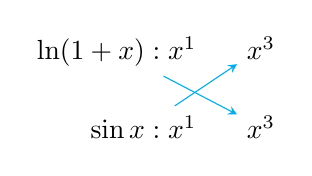
\begin{tikzpicture}[samples=100,>=stealth,]
        \node[below left] (A) at (0,0) {$\sin x:x^1$};
        \node[below left] (B) at (0,1) {$\ln(1+x):x^1$};
        \node[below left] (C) at (1,0) {$x^3$};
        \node[below left] (D) at (1,1) {$x^3$};
        \draw[->,cyan] (A)--(D);
        \draw[->,cyan] (B)--(C);
    \end{tikzpicture}
\end{minipage}
\begin{minipage}{0.3\linewidth}
    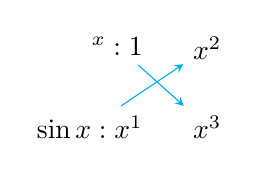
\begin{tikzpicture}[samples=100,>=stealth,]
        \node[below left] (A) at (0,1) {$\e ^x:1$};
        \node[below left] (B) at (0,0) {$\sin x:x^1$};
        \node[below left] (C) at (1,0) {$x^3$};
        \node[below left] (D) at (1,1) {$x^2$};
        \draw[->,cyan] (A)--(C);
        \draw[->,cyan] (B)--(D);
    \end{tikzpicture}
\end{minipage}
\begin{minipage}{0.3\linewidth}
    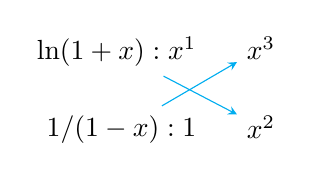
\begin{tikzpicture}[samples=100,>=stealth,]
        \node[below left] (A) at (0,1) {$\ln(1+x):x^1$};
        \node[below left] (B) at (0,0) {$1/(1-x):1$};
        \node[below left] (C) at (1,0) {$x^2$};
        \node[below left] (D) at (1,1) {$x^3$};
        \draw[->,cyan] (A)--(C);
        \draw[->,cyan] (B)--(D);
    \end{tikzpicture}
\end{minipage}
\begin{solution}
    \begin{enumerate}[label=(\arabic{*})]
        \item $\ln(1+x)=x-\dfrac{1}{2}x^2+\dfrac{1}{3}x^3+o(x^3),~\sin x=x-\dfrac{1}{6}x^3+o(x^3)$, 所以
              \begin{flalign*}
                  \ln \left( 1+x\right) \sin x & =\left( x-\dfrac{1}{2}x^{2}+\dfrac{1}{3}x^{3}+o_{1}\left( x^{3}\right) \right) \left( x-\dfrac{1}{6}x^{3}+o_{2}\left( x^{3}\right) \right)      \\
                                               & =x^{2}-\dfrac{1}{6}x^{4}-\dfrac{1}{2}x^{3}+\dfrac{1}{3}x^{4}+o\left( x^{4}\right) =\dfrac{1}{6}x^4-\dfrac{1}{2}x^{3}+x^{2}+o\left( x^{4}\right)
              \end{flalign*}
        \item $\e ^x=1+x+\dfrac{1}{2}x^2+o(x^2),~\sin x=x-\dfrac{1}{6}x^3+o(x^3)$, 所以
              \begin{flalign*}
                  \e ^x\sin x & =\left( 1+x+\dfrac{1}{2}x^{2}+o\left( x^{2}\right) \right) \left( x-\dfrac{1}{6}x^{3}+o\left( x^{3}\right) \right) \\
                              & =x-\dfrac{1}{6}x^{3}+x^{2}+\dfrac{1}{2}x^{3}+o\left( x^{3}\right) =\dfrac{1}{3}x^{3}+x^{2}+x+o\left( x^{3}\right)
              \end{flalign*}
        \item $\ln(1+x)=x-\dfrac{1}{2}x^2+\dfrac{1}{3}x^3+o(x^3),~\dfrac{1}{1-x}=1+x+x^2+o(x^2)$, 所以
              \begin{flalign*}
                  \dfrac{\ln(1+x)}{1-x} & =\left(x-\dfrac{1}{2}x^2+\dfrac{1}{3}x^3+o(x^3)\right)\left(1+x+x^2+o(x^2)\right)                           \\
                                        & =x+x^2+x^3-\dfrac{1}{2}x^2-\dfrac{1}{2}x^3+\dfrac{1}{3}x^3+o(x^3)=\dfrac{5}{6}x^3+\dfrac{1}{2}x^2+x+o(x^3).
              \end{flalign*}
    \end{enumerate}
\end{solution}

\begin{inference}
    $f_1,f_2,\cdots,f_k$ 展开第一个不为 0 的项次数分别为 $m_1,m_2,\cdots,m_k$, 欲使 $f_1f_2\cdots f_k$ 展开到 $p$ 阶,
    则 $f_1,f_2,\cdots,f_k$ 分别需要展开到 $p-(m_2+m_3+\cdots+m_k),p-(m_1+m_3+\cdots+m_k),\cdots,p-(m_2+m_3+\cdots+m_{k-1})$ 阶.
    \label{taylor f1f2f3fk}
\end{inference}
\begin{example}
    \scriptsize\linespread{0.8}
    试用推论 \ref{taylor f1f2f3fk}, 计算例 \ref{liti 111}(12).
\end{example}
\begin{solution}
    \scriptsize\linespread{0.8}
    需要将$\sin kx$ 展开到三阶, 故 $\sin kx=kx-\dfrac{1}{6}(kx)^3+o(x^3)$, 那么
    $$\prod_{k=1}^{n}\sin kx=\prod_{k=1}^{n}\left[kx-\dfrac{1}{6}(kx)^3+o(x^3)\right]~ (x\to0)$$
    在上式中排列组合出 $x$ 的阶数小于等于 $n+2$ 的项, 有
    $$\prod_{k=1}^{n}\sin kx=n!x^n-\sum_{k=1}^{n}\dfrac{1}{6}n!k^2x^{n+2}+o(x^{n+2})=n!x^n-\dfrac{n!x^{n+2}}{6}\sum_{k=1}^{n}k^2+o(x^{n+2})~ (x\to0)$$
    故原式$\displaystyle=\lim\limits_{x\to0}\dfrac{n!x^n-n!x^n+\dfrac{n!x^{n+2}}{6}\displaystyle\sum\limits_{k=1}^{n}k^2+o\qty(x^{n+2})}{x^{n+2}}=\dfrac{n!}{6}\sum_{k=1}^{n}k^2=\dfrac{n(2n+1)}{36}(n+1)!.$
\end{solution}

\paragraph{复合函数的 Taylor 展开}
先确定外函数的展开阶数, 再由各项阶数确定内函数的展开阶数.

\begin{example}
    将下列函数展开到指定的阶数.
    \setcounter{magicrownumbers}{0}
    \begin{table}[H]
        \centering
        \begin{tabular}{l | l}
            (\rownumber{}) $\sin (\sin x)$, 展开到 $3$ 阶. & (\rownumber{}) $\e ^{\tan x}-\e ^{\sin x}$, 展开到 $3$ 阶.         \\
            (\rownumber{}) $\ln\cos x$, 展开到 $6$ 阶.     & (\rownumber{}) $\dfrac{1}{\e }(1+x)^{\frac{1}{x}}$, 展开到 $3$ 阶.
        \end{tabular}
    \end{table}
\end{example}
\begin{solution}
    \begin{enumerate}[label=(\arabic{*})]
        \item 先将外层函数展开到 3 阶,
              \begin{flalign*}
                  \sin(\sin x) & =\sin x-\dfrac{1}{6}\sin^3x+o(\sin^3x)=x-\dfrac{1}{6}x^3+o(x^3)-\dfrac{1}{6}(x+o(x))^3+o(x^3) \\
                               & =x-\dfrac{1}{6}x^3-\dfrac{1}{6}x^3+o(x^3)=x-\dfrac{1}{3}x^3+o(x^3).
              \end{flalign*}
        \item $\e ^{\tan x}-\e ^{\sin x}=\e ^{\tan x}-1-(\e ^{\sin x}-1)$, 先将外层函数展开到 3 阶,
              \begin{flalign*}
                  \e ^{\tan x}-1 & =\tan x+\dfrac{1}{2}\tan ^{2}x+\dfrac{1}{6}\tan ^{3}x+o\left( \tan ^{3}x\right)                                                                                                          \\
                                 & =\left( x+\dfrac{1}{3}x^{3}+o\left( x^{3}\right) \right) +\dfrac{1}{2}\left( x+o\left( x\right) \right) ^{2}+\dfrac{1}{6}\left( x+o\left( x\right) \right) ^{3}+o\left( x^{3}\right)     \\
                                 & =\dfrac{1}{2}x^{3}+\dfrac{1}{2}x^{2}+x+o\left( x^{3}\right)                                                                                                                              \\
                  \e ^{\sin x}-1 & =\sin x+\dfrac{1}{2}\sin ^{2}x+\dfrac{1}{6}\sin ^{3}x+o\left( \sin ^{3}x\right)                                                                                                          \\
                                 & =\left( x^{3}-\dfrac{1}{6}x^{3}+o\left( x^{3}\right) \right) +\dfrac{1}{2}\left( x+o\left( x\right) \right) ^{2}+\dfrac{1}{6}\left( x+o\left( x\right) \right) ^{3}+o\left( x^{3}\right) \\
                                 & =\dfrac{1}{2}x^{2}+x+o\left( x^{3}\right)
              \end{flalign*}
              故 $\e ^{\tan x}-\e ^{\sin x}=\dfrac{1}{2}x^3+o(x^3).$
        \item 先将外层函数展开到 6 阶,
              \begin{flalign*}
                   & \ln\cos x=\dfrac{1}{2}\ln\left(1-\sin^2x\right)=-\dfrac{1}{2}\left(\sin^2x+\dfrac{\sin^4x}{2}+\dfrac{\sin^6x}{3}+o(\sin^3x)\right)                                                                                                                             \\
                   & =-\dfrac{1}{2}\left[\left( x-\dfrac{x^{3}}{3!}+\dfrac{x^{5}}{5!}+o\left( x^{5}\right) \right)^2 +\dfrac{1}{2}\left( x-\dfrac{x^{3}}{3!}+\dfrac{x^{5}}{5!}+0\left( x^{5}\right) \right) ^{4}+\dfrac{1}{3}\left( x+o(x)\right) ^{6} \right]+o\left( x^{6}\right) \\
                   & =-\dfrac{1}{45}x^{6}-\dfrac{1}{12}x^{4}-\dfrac{1}{2}x^{2}+o\left( x^{6}\right) .
              \end{flalign*}
        \item 原式 $=\e ^{\frac{1}{x}\ln(1+x)-1}$, 注意到 $\displaystyle \ln(1+x)=\sum_{n=0}^{\infty}(-1)^n\dfrac{x^{n+1}}{n+1}$, 于是
              \begin{flalign*}
                  \text{原式} & =\e ^{-\frac{x}{2}+\frac{x^2}{3}-\frac{x^3}{4}+o\qty(x^3)}=1+\qty(-\dfrac{x}{2}+\dfrac{x^2}{3}-\dfrac{x^3}{4}+o\qty(x^3))                                 \\
                              & ~  +\dfrac{1}{2}\qty(-\dfrac{x}{2}+\dfrac{x^2}{3}-\dfrac{x^3}{4}+o\qty(x^3))^2+\dfrac{1}{6}\qty(-\dfrac{x}{2}+\dfrac{x^2}{3}-\dfrac{x^3}{4}+o\qty(x^3))^3 \\
                              & =1-\dfrac{1}{2}x+\dfrac{11}{24}x^2-\dfrac{7}{16}x^3+o\qty(x^3).
              \end{flalign*}
    \end{enumerate}
\end{solution}

\begin{example}
    计算下列极限值.
    \setcounter{magicrownumbers}{0}
    \begin{table}[H]
        \centering
        \begin{tabular}{l | l}
            (\rownumber{}) $\displaystyle\lim_{x\to0}\dfrac{\tan\qty(\e ^x-1)-\e ^{\tan x}+1}{x^4}$.                & (\rownumber{}) $\displaystyle\lim_{x\to0}\dfrac{\cos\qty(\sin x)-\e ^{\cos x-1}}{\tan ^2x-\sin ^2x}$.      \\
            (\rownumber{}) $\displaystyle \lim_{x\to0}\dfrac{\ln\qty(1+\sin^2x)-6\qty(\sqrt[3]{2-\cos x}-1)}{x^4}.$ & (\rownumber{}) $\displaystyle \lim_{x\to\infty}\qty[\qty(x-\dfrac{1}{2})^2-x^4\ln^2\qty(1+\dfrac{1}{x})].$
        \end{tabular}
    \end{table}
\end{example}
\begin{solution}
    \begin{enumerate}[label=(\arabic{*})]
        \item 注意到 $$\e ^x=1+x+\dfrac{1}{2}x^2+\dfrac{1}{6}x^3+\dfrac{1}{24}x^4+o\qty(x^4),~\tan x=x+\dfrac{1}{3}x^3+o\qty(x^4)$$
              于是
              \begin{flalign*}
                  \tan\qty(\e ^x-1) & =\e ^x-1+\dfrac{1}{3}\qty(\e ^x-1)^3+o\qty(x^4)                                                                                                   \\
                                    & =x+\dfrac{1}{2}x^2+\dfrac{1}{6}x^3+\dfrac{1}{24}x^4+\dfrac{1}{3}\qty(x+\dfrac{1}{2}x^2+\dfrac{1}{6}x^3+\dfrac{1}{24}x^4+o\qty(x^4))^3+o\qty(x^4)  \\
                                    & =x+\dfrac{1}{2}x^2+\dfrac{1}{6}x^3+\dfrac{1}{24}x^4+\dfrac{1}{3}x^3\qty(1+\dfrac{1}{2}x+\dfrac{1}{6}x^2+\dfrac{1}{24}x^3+o\qty(x^3))^3+o\qty(x^4) \\
                                    & =x+\dfrac{1}{2}x^2+\dfrac{1}{6}x^3+\dfrac{1}{24}x^4+\dfrac{1}{3}x^3+\dfrac{1}{2}x^4+o\qty(x^4)                                                    \\
                                    & =x+\dfrac{1}{2}x^2+\dfrac{1}{2}x^3+\dfrac{13}{24}x^4+o\qty(x^4)
              \end{flalign*}
              \begin{flalign*}
                   & \e ^{\tan x}-1  =\tan x+\dfrac{1}{2}\tan ^2x+\dfrac{1}{6}\tan^3x+\dfrac{1}{24}\tan ^4x+o\qty(x^4)                                                                             \\
                   & =x+\dfrac{x^3}{3}+\dfrac{1}{2}\qty(x+\dfrac{x^3}{3}+o\qty(x^4))^2+\dfrac{1}{6}\qty(x+\dfrac{x^3}{3}+o\qty(x^4))^3+\dfrac{1}{24}\qty(x+\dfrac{x^3}{3}+o\qty(x^4))^4+o\qty(x^4) \\
                   & =x+\dfrac{1}{3}x^3+\dfrac{1}{2}\qty(x^2+\dfrac{2}{3}x^4+o\qty(x^4))+\dfrac{1}{6}\qty(x^3+o\qty(x^4))+\dfrac{1}{24}\qty(x^4+o\qty(x^4))+o\qty(x^4)                             \\
                   & =x+\dfrac{1}{2}x^2+\dfrac{1}{2}x^3+\dfrac{9}{24}x^4+o\qty(x^4)
              \end{flalign*}
              因此$\text{原式}=\dfrac{\dfrac{1}{6}x^4+o\qty(x^4)}{x^4}=\dfrac{1}{6}.$
        \item 与上题同理, 注意到
              $$\cos x=1-\dfrac{1}{2}x^2+\dfrac{1}{24}x^4+o\qty(x^4),~\sin x=x-\dfrac{1}{6}x^3+o\qty(x^4)$$
              $$\tan x=x+\dfrac{1}{3}x^3+o\qty(x^4),~\e ^x=1+x+\dfrac{1}{2}x^2+\dfrac{1}{6}x^3+\dfrac{1}{24}x^4+o\qty(x^4)$$
              于是 \begin{flalign*}
                  \cos \qty(\sin x) & =1-\dfrac{1}{2}\sin^2x+\dfrac{1}{24}\sin^4x+o\qty(x^4)                                                           \\
                                    & =1-\dfrac{1}{2}\qty(x-\dfrac{1}{6}x^3+o\qty(x^4))^2+\dfrac{1}{24}\qty(x-\dfrac{1}{6}x^3+o\qty(x^4))^4+o\qty(x^4) \\
                                    & =1-\dfrac{1}{2}\qty(x^2-\dfrac{1}{3}x^4+o\qty(x^4))+\dfrac{1}{24}x^4+o\qty(x^4)                                  \\
                                    & =1-\dfrac{1}{2}x^2+\dfrac{5}{24}x^4+o\qty(x^4)
              \end{flalign*}
              \begin{flalign*}
                  \e ^{\cos x-1} & =\e ^{-\frac{1}{2}x^2+\frac{1}{24}x^4++o\qty(x^4)}                                                                              \\
                                 & =1+\qty(-\dfrac{1}{2}x^2+\dfrac{1}{24}x^4+o\qty(x^4))+\dfrac{1}{2}\qty(-\dfrac{1}{2}x^2+\dfrac{1}{24}x^4+o\qty(x^4))+o\qty(x^4) \\
                                 & =1-\dfrac{1}{2}x^2+\dfrac{1}{24}x^4+o\qty(x^4)+\dfrac{1}{2}x^4\qty(-\dfrac{1}{2}+\dfrac{1}{24}x^2+o\qty(x^2))^2+o\qty(x^4)      \\
                                 & =1-\dfrac{1}{2}x^2+\dfrac{1}{24}x^4+\dfrac{1}{8}x^4+o\qty(x^4)=1-\dfrac{1}{2}x^2+\dfrac{1}{6}x^4+o\qty(x^4)
              \end{flalign*}
              \begin{flalign*}
                  \tan^2x-\sin^2x & =\qty(x+\dfrac{1}{3}x^3+o\qty(x^4))^2-\qty(x-\dfrac{1}{6}x^3+o\qty(x^4))^2          \\
                                  & =x^2+\dfrac{2}{3}x^4+o\qty(x^4)-\qty(x^2-\dfrac{1}{3}x^4+o\qty(x^4))=x^4+o\qty(x^4)
              \end{flalign*}
              于是原式 $=\displaystyle\lim_{x\to0}\dfrac{1-\dfrac{1}{2}x^2+\dfrac{5}{24}x^4+o\qty(x^4)-\qty(1-\dfrac{1}{2}x^2+\dfrac{1}{6}x^4+o\qty(x^4))}{x^4+o\qty(x^4)}=\dfrac{1}{24}.$
        \item $\ln\qty(1+\sin^2x)=\sin^2x-\dfrac{1}{2}\sin^4x+o\qty(x^4)$, 且 $\sin x=x-\dfrac{1}{6}x^3+o\qty(x^4)$, 于是
              \begin{flalign*}
                  \ln\qty(1+\sin^2x) & =\qty(x-\dfrac{1}{6}x^3)^2-\dfrac{1}{2}\qty(x-\dfrac{1}{6}x^3)^4+o\qty(x^4)                                       \\
                                     & =x^2\qty(1-\dfrac{1}{6}x^2)^2-\dfrac{1}{2}x^4\qty(1-\dfrac{1}{6}x^2)^4+o\qty(x^4) =x^2-\dfrac{5}{6}x^4+o\qty(x^4)
              \end{flalign*}
              另一方面,
              \begin{flalign*}
                  \sqrt[3]{2-\cos x}-1 & =\sqrt[3]{1+(1-\cos x)}-1=\dfrac{1}{3}(1-\cos x)+\dfrac{\dfrac{1}{3}\cdot\qty(-\dfrac{2}{3})}{2!}(1-\cos x)^2                                                    \\
                                       & =\dfrac{1}{3}\qty(\dfrac{x^2}{2}-\dfrac{x^4}{24}+o\qty(x^4))-\dfrac{1}{9}\qty(\dfrac{x^2}{2}+o\qty(x^4))^2+o\qty(x^4)=\dfrac{1}{6}x^2-\dfrac{x^4}{24}+o\qty(x^4)
              \end{flalign*}
              于是原式 $=\lim_{x\to0}\dfrac{-\dfrac{7}{12}x^4+o\qty(x^4)}{x^4}=-\dfrac{7}{12}.$
        \item \textbf{法一: }利用 L'Hospital 法则计算极限
              \begin{flalign*}
                  I & =\lim_{x\to\infty}x^2\qty[1-\dfrac{1}{2x}+\ln\qty(1+\dfrac{1}{x})]\qty[1-\dfrac{1}{2x}-\ln\qty(1+\dfrac{1}{x})]
                  \xlongequal{\frac{1}{x}=t}\lim_{t\to0}\qty[1-\dfrac{t}{2}+\dfrac{\ln(1+t)}{t}]\cdot\dfrac{t-\dfrac{t^2}{2}-\ln(1+t)}{t^3}                    \\
                    & \xlongequal{L'}\lim_{t\to0}\dfrac{2-2t+\dfrac{2}{1+t}}{2}\cdot\dfrac{1-t-\dfrac{1}{1+t}}{3t^2}=2\times\qty(-\dfrac{1}{3})=-\dfrac{2}{3}.
              \end{flalign*}
              \textbf{法二: }对 $\ln\qty(1+\dfrac{1}{x}),~x\to\infty$ 进行 Taylor 展开, 有
              \begin{flalign*}
                  I & =\lim_{x\to\infty}\qty[\qty(x-\dfrac{1}{2})^2-x^4\qty(\dfrac{1}{x}-\dfrac{1}{2x^2}+\dfrac{1}{3x^3}+o\qty(x^{-4}))^2]=\lim_{x\to\infty}\qty[\qty(x-\dfrac{1}{2})^2-x^2\qty(1-\dfrac{1}{2x}+\dfrac{1}{3x^2}+o\qty(x^{-3}))^2] \\
                    & =\lim_{x\to\infty}\qty[\qty(x-\dfrac{1}{2})^2-\qty(x-\dfrac{1}{2}+\dfrac{1}{3x})^2]=\lim_{x\to\infty}\qty(x-\dfrac{1}{2}+x-\dfrac{1}{2}+\dfrac{1}{3x})\qty(x-\dfrac{1}{2}-x+\dfrac{1}{2}-\dfrac{1}{3x})                     \\
                    & =\lim_{x\to\infty}\dfrac{-6x^2+3x-1}{9x^2}=-\dfrac{2}{3}.
              \end{flalign*}
    \end{enumerate}
\end{solution}

\begin{example}
    计算极限 $\displaystyle\lim_{x\to0}\qty[\dfrac{1}{x\ln(1+x)}-\dfrac{2+x}{2x^2}].$
\end{example}
\begin{solution}
    对 $\ln(1+x)$ 进行 Taylor 展开, 有 $\ln(1+x)=x-\dfrac{x^2}{2}+\dfrac{x^3}{3}+o\qty(x^4)$, 于是
    \begin{flalign*}
        \text{原式} & =\lim_{x\to0}\qty[\dfrac{1}{x\qty(x-\dfrac{x^2}{2}+\dfrac{x^3}{3})}-\dfrac{2+x}{2x^2}]=\lim_{x\to0}\qty[\dfrac{12}{2x^2\qty(6-3x+2x^2)}-\dfrac{2+x}{2x^2}] \\
                    & =\lim_{x\to0}\dfrac{12-(2+x)(6-3x+2x^2)}{2x^2\qty(6-3x+2x^2)}=-\lim_{x\to0}\dfrac{2x+1}{2\qty(6-3x+2x^2)}=-\dfrac{1}{12}.
    \end{flalign*}
\end{solution}

\begin{example}
    设函数 $f(x)$ 在区间 $(0,+\infty)$ 上三阶可导, 满足
    $$\lim_{x\to+\infty}\dfrac{f'(x)f'''(x)}{\qty[f''(x)]^2}=a\neq 1~  f^{(k)}(x)>0,~k=0,1,2$$
    求极限 $\displaystyle\lim_{x\to+\infty}\dfrac{f(x)f''(x)}{\qty[f'(x)]^2}.$
\end{example}
\begin{solution}
    注意到
    \begin{flalign*}
        \lim_{x\to+\infty}\dfrac{f'(x)f'''(x)}{\qty[f''(x)]^2} & =\lim_{x\to+\infty}\dfrac{\qty[f''(x)]^2-\qty[f''(x)]^2+f'(x)f'''(x)}{\qty[f''(x)]^2}                                      \\
                                                               & =1-\lim_{x\to+\infty}\dfrac{\qty[f''(x)]^2-f'(x)f'''(x)}{\qty[f''(x)]^2}=1-\lim_{x\to+\infty}\dv{x}(\dfrac{f'(x)}{f''(x)})
    \end{flalign*}
    于是 $\displaystyle\lim_{x\to+\infty}\dv{x}(\dfrac{f'(x)}{f''(x)})=1-a$, 并且
    $$\lim_{x\to+\infty}\dfrac{f(x)f''(x)}{\qty[f'(x)]^2}=\dfrac{1}{\dfrac{f'(x)}{xf''(x)}\cdot\dfrac{xf''(x)}{f(x)}}$$
    利用 L'Hospital 法则, 得
    $$\lim_{x\to\infty}\dfrac{f'(x)}{xf''(x)}=\lim_{x\to\infty}\dfrac{\dfrac{f'(x)}{f''(x)}}{x}\xlongequal{L'}\lim_{x\to\infty}\dv{x}(\dfrac{f'(x)}{f''(x)})=1-a$$
    注意到 $\dfrac{f'(x)}{xf''(x)}>0~ (0<x<+\infty)$, 故由极限的保号性知, $1-a\geqslant 0$, 但 $a\neq 1$, 所以 $a<1$; 另一方面,
    对 $\forall x\in(0,+\infty)$ 及 $\forall h>0$, 由 Taylor 公式, 得
    $$f(x+h)=f(x)+f'(x)h+\dfrac{1}{2!}f''(\xi)h^2>f(x)+f'(x)h~  \xi\in(x,x+h)$$
    所以 $\displaystyle\lim_{h\to\infty}f(x+h)=+\infty$, 即 $\displaystyle\lim_{x\to\infty}f(x)=+\infty$, 于是利用 L'Hospital 法则, 得
    $$\lim_{x\to+\infty}\dfrac{xf'(x)}{f(x)}\xlongequal{L'}\lim_{x\to+\infty}\dfrac{f'(x)+xf''(x)}{f'(x)}=1+\lim_{x\to+\infty}\dfrac{xf''(x)}{f'(x)}=1+\dfrac{1}{1-a}=\dfrac{2-a}{1-a}$$
    因此 $$\lim_{x\to+\infty}\dfrac{f(x)f''(x)}{\qty[f'(x)]^2}=\dfrac{1}{\lim\limits_{x\to+\infty}\dfrac{f'(x)}{xf''(x)}\cdot\lim\limits_{x\to+\infty}\dfrac{xf'(x)}{f(x)}}=\dfrac{1}{2-a}.$$
\end{solution}

% 例 3.3.19 设函数  f  在  (0,+\infty)  上可微, 且  f^{\prime}(x)=O(x)(  当  x \to+\infty  时  ) , 试证:  f(x)=O\left(x^{2}\right)  (当  x \to+\infty  时). (中国科学技术大学)
% 证 已知  \frac{f^{\prime}(x)}{x}=O(1)(x \to+\infty) , 取  x_{0}>0 , 则  \forall x>x_{0} , 有
% 
% f(x)=f\left(x_{0}\right)+f^{\prime}(\xi)\left(x-x_{0}\right)\left(x_{0}<\xi<x\right),\left|\frac{\xi}{x}\right| \leqslant 1,\left|\frac{x-x_{0}}{x}\right| \leqslant 1
% 
% 故  ~  \frac{f(x)}{x^{2}}=\frac{f\left(x_{0}\right)}{x^{2}}+\left(\frac{f^{\prime}(\xi)}{\xi}\right)\left(\frac{\xi}{x}\right)\left(\frac{x-x_{0}}{x}\right)=o(1)+O(1)=O(1) ,
% 即
% 
% f(x)=O\left(x^{2}\right) \text { (当 } x \to+\infty \text { 时). }
% 
% new  \succsim  例 3.3.20 设  x_{n}=f\left(\frac{1}{n^{2}}\right)+f\left(\frac{2}{n^{2}}\right)+\cdots+f\left(\frac{n}{n^{2}}\right) , 其中  f(x)  在  x=0  处有连 续导数, 且  f(0)=0, f^{\prime}(0)=1 . 试证  : \lim _{n \to \infty} x_{n}  存在,并求极限值. (武汉大学)
% 注  f(x)  在  x=0  处有连续导数, 意指:  f(x)  在  x=0  处及其附近有导数, 并且导 函数  f^{\prime}(x)  至少在  x=0  处连续.
% 证 I 因  f(0)=0, f^{\prime}(0)=1 , 应用 Taylor 公式, 得
% 
% \begin{array}{l}
% x_{n}=\sum_{i=1}^{n} f\left(\frac{i}{n^{2}}\right)=\sum_{i=1}^{n}\left[f(0)+f^{\prime}(0) \frac{i}{n^{2}}+o\left(\frac{i}{n^{2}}\right)\right]=\sum_{i=1}^{n}\left[\frac{i}{n^{2}}+o\left(\frac{i}{n^{2}}\right)\right] \\
% =\sum_{i=1}^{n} \frac{i}{n^{2}}+\sum_{i=1}^{n} o\left(\frac{i}{n^{2}}\right) \\
% \stackrel{\text { 见注 }}{=} \frac{n(n+1)}{2 n^{2}}+\frac{n(n+1)}{2 n^{2}} o(1) \underset{n \to \infty}{\longrightarrow} \frac{1}{2} \text {. } \\
% \end{array}
% 
% 注 当  n \to \infty  时,  o(1)  代表一个无穷小量,且  o\left(\frac{i}{n^{2}}\right)=\frac{i}{n^{2}} o(1) . 因此
% 
% \begin{aligned}
% \sum_{i=1}^{n} o\left(\frac{i}{n^{2}}\right) & =\sum_{i=1}^{n} \frac{i}{n^{2}} o(1)=\frac{1}{n^{2}} \sum_{i=1}^{n} i \cdot o(1) \\
% & =\frac{1}{n^{2}}[o(1)+2 o(1)+3 o(1)+\cdots+n o(1)]
% \end{aligned}

\subsubsection{Lagrange 中值定理}

\begin{theorem}[Lagrange 中值定理]
    \index{Lagrange 中值定理}若 $ f(x) $ 在 $ [a, b] $ 上连续, 在 $ (a, b) $ 内可导, 则 $ \forall x_{1}, x_{2} \in[a, b], \exists \xi \in\left(x_{1}, x_{2}\right) $, 使得
    $$f\left(x_{2}\right)-f\left(x_{1}\right)=f^{\prime}(\xi)\cdot(x_{2}-x_{1}) .$$
\end{theorem}

\begin{example}
    计算 $\displaystyle\lim_{x\to0}\dfrac{\cos x-\cos\qty[2\ln(1+x)]}{x^2}.$
\end{example}
\begin{errorSolution}
    由 Lagrange 中值定理, $\cos x-\cos\qty[2\ln(1+x)]=\qty[2\ln(1+x)-x]\sin\xi$, 其中 $\xi$ 介于 $x$ 与 $2\ln(1+x)$ 之间, 因此
    $$\lim_{x\to0}\dfrac{\cos x-\cos\qty[2\ln(1+x)]}{x^2}=\lim_{x\to0}\dfrac{\qty[2\ln(1+x)-x]\sin\xi}{x^2}=\lim_{x\to0}\dfrac{\qty[2x+o(x)-x]}{x}=1$$
    \textbf{错因: }当 $x\to0^+,~x<\xi<2\ln(1+x)\Rightarrow 1\gets\dfrac{x}{x}<\dfrac{\xi}{x}<\dfrac{2\ln(1+x)}{x}\to 2$, 左右极限值不相等, 故不能由夹逼准则得 $\sin\xi\sim\xi$, 同理可得 $x\to0^-$ 情况相同.\\
\end{errorSolution}
\begin{solution}
    当 $x\to0$ 时, $\cos [2\ln(1+x)]\to1$, 于是原式可改写为 $$\lim_{x\to0}\qty[\dfrac{\cos x-1}{x^2}+\dfrac{1-\cos(2\ln(1+x))}{x^2}]=\lim_{x\to0}\dfrac{\cos x-1}{x^2}+\lim_{x\to0}\dfrac{1-\cos(2\ln(1+x))}{x^2}=-\dfrac{1}{2}+2=\dfrac{3}{2}.$$
\end{solution}

\begin{example}
    已知 $\displaystyle\lim_{n\to\infty}\dfrac{n^{\alpha}}{n^\beta-(n-1)^\beta}=2023$, 求 $\alpha,\beta$ 的值.
    \begin{tasks}(2)
        \task $\alpha=-\dfrac{2022}{2023},~\beta=\dfrac{1}{2023}.$
        \task $\alpha=-\dfrac{2023}{2022},~\beta=\dfrac{1}{2022}.$
        \task $\alpha=-\dfrac{2022}{2023},~\beta=\dfrac{1}{2022}.$
        \task $\alpha=-\dfrac{2023}{2022},~\beta=\dfrac{1}{2023}.$
    \end{tasks}
\end{example}
\begin{solution}
    设 $f(x)=x^\beta$, 那么由 Lagrange 中值定理, 有 $$f(n)-f(n-1)=\beta\xi_n^{\beta-1}$$
    那么极限式改写为 $\displaystyle\lim_{n\to\infty}\dfrac{n^\alpha}{\beta \xi_n^{\beta-1}}=2023$,
    且 $\dfrac{n}{\xi_n}\to1(n\to\infty)$, 于是 $\begin{cases}
            \dfrac{1}{\beta}=2023 \\\alpha=\beta-1
        \end{cases}$ 解得选 A.
\end{solution}

\begin{example}
    用 Lagrange 中值定理求下列极限值.
    \setcounter{magicrownumbers}{0}
    \begin{table}[H]
        \centering
        \begin{tabular}{l | l | l}
            (\rownumber{}) $\displaystyle\lim_{x\to+\infty}\left(\sqrt[6]{x^6+x^5}-\sqrt[6]{x^6-x^5}\right).$ & (\rownumber{}) $\displaystyle\lim_{n\to \infty}\left(\cos\frac{\theta}{n}\right)^n.$ & (\rownumber{}) $\displaystyle\lim_{n\to \infty}\tan ^n\left(\frac{\pi}{4}+\frac{1}{n}\right).$ \\
            (\rownumber{}) $\displaystyle\lim_{x\to0}\left(\frac{1}{x^2}-\cot^2x\right).$                     & (\rownumber{}) $\displaystyle\lim_{x\to0}\frac{\sqrt{1-x^2}-\sqrt{1-4x^2}}{x^2}.$    & (\rownumber{}) $\displaystyle\lim_{x\to0}\frac{\e ^{x^2}-\e ^{2-2\cos x}}{x^4}.$
        \end{tabular}
    \end{table}
\end{example}
\begin{solution}
    \begin{enumerate}[label=(\arabic*)]
        \item $\displaystyle\text{原式}=\lim_{x\to+\infty}\frac{1}{6}\xi^{-\frac{5}{6}}\cdot(2x^5)=\frac{1}{3}$, $\xi\to x^6$.
        \item $\displaystyle\text{原式}=\exp\lim_{n\to\infty}n\ln\cos\frac{\theta}{n}=\exp\lim_{n\to\infty}n\left(\cos\frac{\theta}{n}-1\right)=\exp\lim_{n\to\infty}n\cdot\frac{\theta}{n}\cdot(-\sin\xi)=\e ^0=1$, $\xi\to 0$.
        \item $\displaystyle\text{原式}=\e ^{\lim\limits_{n\to\infty}n\ln\tan\left(\frac{\pi}{4}+\frac{1}{n}\right)}=\exp\lim_{n\to\infty}n\left[\tan\left(\frac{\pi}{4}+\frac{1}{n}\right)-1\right]=\exp\lim_{n\to\infty}\sec^2\xi=\e ^2$, $\displaystyle\xi\to\frac{\pi}{4}$.
        \item 先用 Lagrange 中值定理, 再用 Taylor 展开.
              \begin{flalign*}
                  \text{原式} & =\lim_{x\to0}\frac{\sin^2x-x^2\cos^2x}{x^2\sin^2x}=\lim_{x\to0}\frac{2\ln\sin x-2\ln(x\cos x)}{x^2}=2\lim_{x\to0}\frac{\sin x-x\cos x}{x^2\cdot\xi} \\
                              & =2\lim_{x\to0}\frac{x-\dfrac{x^3}{6}-x\left(1-\dfrac{x^2}{2}\right)+o\left(x^3\right)}{x^2\cdot\xi}=\frac{2}{3},~\xi\to x.
              \end{flalign*}
        \item $\displaystyle\text{原式}=\lim_{x\to0}\frac{3x^2\dfrac{1}{2\sqrt{\xi}}}{x^2}=\frac{3}{2}$, $\xi\to1$.
        \item $\displaystyle\text{原式}=\lim_{x\to0}\frac{\e ^\xi\left(x^2-2+2\cos x\right)}{x^4}=\lim_{x\to0}\frac{x^2-2+2\left(1-\dfrac{x^2}{2!}+\dfrac{x^4}{4!}+o\left(x^4\right)\right)}{x^4}=\frac{1}{12}$, $\xi\to0$.
    \end{enumerate}
\end{solution}

\begin{example}
    设 $f(x)$ 在 $x=0$ 二阶可微且 $f'(0)=0,~f''(0)=1$, 计算极限 $\displaystyle\lim_{x\to0}\dfrac{f(x)-f(\ln(1+x))}{x^3}.$
\end{example}
\begin{solution}
    显然 $f$ 在 $x=0$ 邻域内一阶可微, 因此由 Lagrange 中值定理,
    $$\lim_{x\to0}\dfrac{f(x)-f(\ln(1+x))}{x^3}=\lim_{x\to0}\dfrac{[x-\ln(1+x)]f'(\xi_x)}{x^3}=\dfrac{1}{2}\lim_{x\to0}\dfrac{f'(\xi_x)}{x}=\dfrac{1}{2}\lim_{x\to0}\dfrac{f'(\xi_x)-f'(0)}{\xi_x}\cdot\dfrac{\xi_x}{x}=\dfrac{1}{2}f''(0)=\dfrac{1}{2}$$
    其中
    \begin{flalign*}
        1 & =\lim_{x\to0^+}\dfrac{\ln(1+x)}{x}\leqslant \lim_{x\to0^+}\dfrac{\xi_x}{x}\leqslant \lim_{x\to0^+}\dfrac{x}{x}=1  \\
        1 & =\lim_{x\to0^-}\dfrac{x}{x}\leqslant \lim_{x\to0^-}\dfrac{\xi_x}{x}\leqslant \lim_{x\to0^-}\dfrac{\ln(1+x)}{x}=1.
    \end{flalign*}
\end{solution}

\begin{example}[2011 数一]
    求极限 $\displaystyle\lim_{x\to0}\qty[\dfrac{\ln(1+x)}{x}]^{\frac{1}{\e^x-1}}.$
\end{example}
\begin{solution}
    令 $y=\qty[\dfrac{\ln(1+x)}{x}]^{\frac{1}{\e^x-1}}$, 则 $\ln y=\dfrac{\ln(\ln(x+1))-\ln x}{\e^x-1}$, 而
    \begin{flalign*}
        \lim_{x\to0^+}\ln y=\lim_{x\to0^+}\dfrac{\ln(\ln(x+1))-\ln x}{\e^x-1}=\lim_{x\to0^+}\dfrac{\ln(\ln(x+1))-\ln x}{x}
    \end{flalign*}
    由 Lagrange 中值定理, 令 $f(x)=\ln x$ 那么 $f(1+\ln x)-f(x)=\dfrac{\ln(1+x)-x}{\xi_x}$, 其中 $\xi_x$ 介于 $x$ 与 $\ln(1+x)$ 之间,
    于是 $$\lim_{x\to0^+}\ln y=\lim_{x\to0^+}\dfrac{\ln(1+x)-x}{x\cdot \xi_x}=\lim_{x\to0^+}\dfrac{-\dfrac{1}{2}x^2}{x^2}=-\dfrac{1}{2}$$
    当 $x<0$ 时, $\ln y=\dfrac{\ln[-\ln(1+x)]-\ln(-x)}{\e^x-1}$ 同样可得 $\displaystyle\lim_{x\to0^-}\ln y=-\dfrac{1}{2}$, 于是原极限为 $\e^{-\frac{1}{2}}.$
\end{solution}

\begin{example}[第三届数学竞赛决赛]
    证明: $\displaystyle\lim_{n\to\infty}\int_0^1\frac{n}{n^2x^2+1}\e ^{x^2}\dd x=\frac{\pi}{2}.$
\end{example}
\begin{proof}
    对函数 $\displaystyle f(x)=\e ^{x^2}$ 在区间 $[0,x]~ (0\leqslant x\leqslant 1)$ 上应用拉格朗日中值定理, $\exists \xi\in(0,x)$, 使得 $f(x)-f(0)=f'(\xi)x$, 即
    $$\e ^{x^2}-1=2\xi\e ^{\xi^2}x\Rightarrow 1\leqslant \e ^{x^2}=1+2\xi\e ^{\xi^2}x\leqslant 1+2\e x$$
    于是 $$\frac{n}{n^2x^2+1}\leqslant \frac{n}{n^2x^2+1}\e ^{x^2}\leqslant \frac{n}{n^2x^2+1}+\frac{2\e nx}{n^2x^2+1}$$
    应用定积分的保号性, 有
    $$\int_0^1\frac{n}{n^2x^2+1}\e ^{x^2}\dd x\geqslant \int_0^1\frac{n}{n^2x^2+1}\dd x=\arctan nx\Bigl |_0^1=\arctan n$$
    \begin{flalign*}
        \int_0^1\frac{n}{n^2x^2+1}\e ^{x^2}\dd x  \leqslant \int_0^1\left(\frac{n}{n^2x^2+1}+\frac{2\e nx}{n^2x^2+1}\right)\dd x
        =\arctan nx\Bigl |_0^1+\frac{\e }{n}\ln\left(1+n^2x^2\right)\Bigl |_0^1=\arctan n+\frac{\e }{n}\ln\left(1+n^2\right)
    \end{flalign*}
    又因为 $\displaystyle \lim_{n\to\infty}\arctan n=\frac{\pi}{2},~\lim_{n\to\infty}\left[\arctan n+\frac{\e }{n}\ln\left(1+n^2\right)\right]=\frac{\pi}{2}$, 故由夹逼准则, 等式成立.
\end{proof}

\begin{example}
    计算极限 $\displaystyle \lim_{x\to+\infty}(x+1)\qty[\ln\qty(x^2+x)-2\ln(1+x)].$
\end{example}
\begin{solution}
    \textbf{法一: }利用重要极限 $\displaystyle \lim_{x\to\infty}\qty(1+\dfrac{1}{x})^x=\e $, 改写极限式, 有
    \begin{flalign*}
        \text {原式} & =\lim _{x \to+\infty}(x+1) \ln \frac{x^{2}+x}{(1+x)^{2}}=\lim _{x \to+\infty}(x+1) \ln \frac{x^{2}+x}{x^{2}+2 x+1}
        =\lim _{x \to+\infty}(x+1) \ln \left(1+\frac{-x-1}{x^{2}+2 x+1}\right)                                                                    \\
                     & =\lim _{x \to+\infty}(x+1) \cdot \frac{-x-1}{x^{2}+2 x+1}=-\lim _{x \to+\infty} \frac{(x+1)^{2}}{x^{2}+2 x+1}=-1 .
    \end{flalign*}
    \textbf{法二: }利用 Lagrange 中值定理: 设 $ f(x)=\ln x $, 则 $ \exists \xi $ 介于 $ x^{2}+x $ 与 $ x^{2}+2 x+1 $, 使得
    $$\frac{f\left(x^{2}+x\right)-f\left(x^{2}+2 x+1\right)}{\left(x^{2}+x\right)-\left(x^{2}+2 x+1\right)}=f^{\prime}(\xi)=\frac{1}{\xi}, \xi \to \infty $$
    即 $ \ln \left(x^{2}+x\right)-\ln \left(x^{2}+2 x+1\right)=-\dfrac{1}{\xi}(x+1) $, 所以
    \begin{flalign*}
          & \lim _{x \to+\infty}(x+1)\left[\ln \left(x^{2}+x\right)-2 \ln (1+x)\right] =\lim _{x \to+\infty}(x+1)\left[\ln \left(x^{2}+x\right)-\ln \left(x^{2}+2 x+1\right)\right] \\
        = & \lim _{x \to+\infty}(x+1)\left[-\frac{1}{\xi}(x+1)\right]=-\lim _{x \to+\infty} \frac{(x+1)^{2}}{\xi}
    \end{flalign*}
    因为 $ \xi $ 介于 $ x^{2}+x $ 与 $ x^{2}+2 x+1 $, 由夹逼准则可知:
    $$\lim _{x \to+\infty}(x+1)\left[\ln \left(x^{2}+x\right)-2 \ln (1+x)\right]=-1$$
    \textbf{法三: }由 L'Hospital 法则可知: 注意到
    $$\lim _{x \to+\infty}\left[\ln \left(x^{2}+x\right)-2 \ln (1+x)\right]=0, \lim _{x \to \infty} \frac{1}{x+1}=0$$
    记 $ \displaystyle I=\lim _{x \to+\infty}(x+1)\left[\ln \left(x^{2}+x\right)-2 \ln (1+x)\right] $, 则
    \begin{flalign*}
        I & =\lim _{x \to+\infty} \dfrac{\ln \left(x^{2}+x\right)-2 \ln (1+x)}{\dfrac{1}{x+1}} =\lim _{x \to+\infty} \dfrac{\dfrac{2 x+1}{x^{2}+x}-\dfrac{2}{1+x}}{-\dfrac{1}{(x+1)^{2}}} \\
          & =-\lim _{x \to+\infty}\left[\dfrac{2 x+1}{x^{2}+x}-\dfrac{2 x}{(1+x) x}\right](x+1)^{2} =-\lim _{x \to+\infty} \dfrac{(x+1)^{2}}{x^{2}+x} =-1
    \end{flalign*}
    所以 $ \displaystyle \lim _{x \to+\infty}(x+1)\left[\ln \left(x^{2}+x\right)-2 \ln (1+x)\right]=-1 .$\\
    \textbf{法四: }$\ln \left(x^{2}+x\right) $ 和 $ \ln (1+x) $ 在 $ x \to+\infty $ 的渐近展开式. 注意到:
    $$\ln \left(x^{2}+x\right)=2 \ln x+\frac{1}{x}+o\left(\frac{1}{x}\right),~\ln (1+x)=\ln x+\frac{1}{x}+o\left(\frac{1}{x}\right)$$
    所以
    \begin{flalign*}
        \lim _{x \to+\infty}(x+1)\left[\ln \left(x^{2}+x\right)-2 \ln (1+x)\right] & =\lim _{x \to+\infty}(x+1)\left[2 \ln x+\frac{1}{x}+o\left(\frac{1}{x}\right)-2\left(\ln x+\frac{1}{x}+o\left(\frac{1}{x}\right)\right)\right] \\
                                                                                           & =  \lim _{x \to+\infty}(x+1)\left[-\frac{1}{x}+o\left(\frac{1}{x}\right)\right]=-1 .
    \end{flalign*}
\end{solution}

\begin{example}
    求极限 $\displaystyle I=\lim_{x\to\infty}x^2\qty[\e^{\qty(1+\frac{1}{x})^x}-\qty(1+\dfrac{1}{x})^{\e x}].$
\end{example}
\begin{solution}
    作变量代换: $t=\dfrac{1}{x}$, 则有
    \begin{flalign*}
        I=\lim_{t\to0}\dfrac{\e^{(1+t)^{t^{-1}}}-(1+t)^{\frac{\e}{t}}}{t^2}=\lim_{t\to0}\dfrac{\e^{(1+t)^{t^{-1}}}-\e^{\frac{\e\ln(1+t)}{t}}}{t^2}
    \end{flalign*}
    令 $f(t)=(1+t)^{t^{-1}},~g(t)=\dfrac{\e\ln(1+t)}{t}$, 则 $\displaystyle\lim_{t\to0}f(t)=\lim_{t\to0}g(t)=0$, 由 Lagrange 中值定理, 得
    $$\e^{f(t)}-\e^{g(t)}=\e^{\xi}(f(t)-g(t))$$
    其中 $\xi$ 介于 $f(t)$ 与 $g(t)$ 之间, 当 $t\to0$ 时, $\xi\to\e$, 所以 $\e^{f(t)}-\e^{g(t)}\sim\e^{\e}[f(t)-g(t)]$, 故
    $$I=\e^{\e}\lim_{t\to0}\dfrac{f(t)-g(t)}{t^2}=\e^{\e+1}\lim_{t\to0}\dfrac{\e^{\frac{\ln(1+t)}{t}-1}-\dfrac{\ln(1+t)}{t}}{t^2}$$
    记 $\alpha(t)=\dfrac{\ln(1+t)}{t}-1~ (t\to0,\alpha(t)\to0)$, 由 $\e^{\alpha(t)}$ 的 Taylor 展开, 得
    $$\e^{\alpha(t)}=1+\alpha(t)+\dfrac{1}{2!}\alpha^2(t)+o\qty(\alpha^2(t))=\dfrac{\ln(1+t)}{t}+\dfrac{1}{2}\qty[\dfrac{\ln(1+t)-t}{t}]^2+o\qty(\alpha^2(t))$$
    因此 $$I=\e^{\e+1}\lim_{t\to0}\dfrac{1}{2}\cdot\dfrac{\qty[\ln(1+t)-t]^2}{t^4}=\dfrac{1}{2}\e^{\e+1}\lim_{t\to0}\dfrac{\qty[-\dfrac{t^2}{2}+o\qty(t^2)]^2}{t^4}=\dfrac{1}{8}\e^{\e+1}.$$
\end{solution}

\begin{example}
    求极限 $\displaystyle\lim_{x\to0}\dfrac{\qty(\sin x+\e^{\tan x})^{\frac{1}{x}}-\qty(\tan x+\e^{\sin x})^{\frac{1}{x}}}{x^3}$
\end{example}
\begin{solution}
    改写极限式, 有
    \begin{flalign*}
        I & =\lim_{x\to0}\dfrac{\qty(\sin x+\e^{\tan x})^{\frac{1}{x}}\cdot\dfrac{1}{x}\qty[\ln\qty(\sin x+\e^{\tan x})-\ln\qty(\tan x+\e^{\sin x})]}{x^3} \\
          & =\lim_{x\to0}\qty(\sin x+\e^{\tan x})^{\frac{1}{x}}\cdot\lim_{x\to0}\dfrac{\e^{\tan x}-\tan x-\qty(\e^{\sin x}-\sin x)}{x^4}                   \\
          & =\exp\lim_{x\to0}\dfrac{1}{x}\ln\qty(\sin x+\e^{\tan x})\cdot\lim_{x\to0}\dfrac{(\tan x-\sin x)f'(\xi_x)}{x^4}                                 \\
    \end{flalign*}
    其中 $$\displaystyle\lim_{x\to0}\dfrac{1}{x}\ln\qty(\sin x+\e^{\tan x})=\exp\lim_{x\to0}\dfrac{1}{x}\qty(\sin x+\e^{\tan x}-1)=\exp\lim_{x\to0}\dfrac{\sin x+\tan x}{x}=\e^2$$
    $\xi_x$ 介于 $\sin x$ 与 $\tan x$ 之间, 并且
    $$\lim_{x\to0}\dfrac{(\tan x-\sin x)f'(\xi_x)}{x^4}=\lim_{x\to0}\dfrac{\dfrac{1}{2}x^3f'(\xi_x)}{x^4}=\dfrac{1}{2}\lim_{x\to0}\dfrac{f'(\xi_x)}{x}=\dfrac{1}{2}$$
    这是因为 $f'(x)=\e^x-1\to x~ (x\to0)$, 以及当 $x\to0^+$ 时, $$0\gets\sin x<\xi_x<\tan x\to0$$
    当 $x\to0^-$ 时, $$0\gets\tan x<\xi_x<\sin x\to0$$
    于是 $\displaystyle\lim_{x\to0}\dfrac{f'(\xi_x)}{x}=1$, 综上原式 $=\dfrac{\e^2}{2}.$
\end{solution}

\begin{example}
    设 $f(x)$ 在 $x=a$ 的某邻域内有三阶连续导数, 且 $f'(a)\neq0$, 令 $$\varphi(x)=\qty[\dfrac{f'(x)+f'(a)}{2f(x)-2f(a)}]^2-\qty(\dfrac{1}{x-a})^2$$
    计算极限 $\displaystyle\lim_{x\to a}\varphi(x).$
\end{example}
\begin{solution}
    考虑 $f(x)$ 在 $x=a$ 处的 Taylor 展开, $$f(x)=f(a)+f'(a)(x-a)+\dfrac{1}{2!}f''(a)(x-a)^2+\dfrac{1}{3!}f'''(\xi)(x-a)^3$$
    于是 $$2f(x)-2f(a)=2f'(a)(x-a)+f''(a)(x-a)^2+\dfrac{1}{3}f'''(\xi)(x-a)^3$$
    其中 $\xi$ 介于 $x$ 与 $a$ 之间, 同理, 考虑 $f'(x)$ 在 $x=a$ 处的 Taylor 展开, $$f'(x)=f'(a)+f''(a)(x-a)+\dfrac{1}{2!}f'''(\eta)(x-a)^2$$
    于是 $$f'(x)+f'(a)=2f'(a)+f''(a)(x-a)+\dfrac{1}{2}f'''(\eta)(x-a)^2$$
    其中 $\eta$ 介于 $x$ 与 $a$ 之间, 将两式代入极限式, 并通分, 于是分子为
    \begin{flalign*}
          & (x-a)^2\qty[2f'(a)+f''(a)(x-a)+\dfrac{f'''(\eta)}{2}(x-a)^2]^2
        -  \qty[2f'(a)(x-a)+f''(a)(x-a)^2+\dfrac{f'''(\xi)}{3}(x-a)^3]^2                   \\
        = & f'(a)\left[2f'''(\eta)-\dfrac{4}{3}f'''(\xi)\right] (x-a)^{4} + o\qty((x-a)^4)
    \end{flalign*}
    分母为
    \begin{flalign*}
        \qty[2f'(a)+f''(a)(x-a)+\dfrac{f'''(\xi)}{3}(x-a)^2]^2(x-a)^4=4\qty[f'(a)]^2(x-a)^4+o\qty((x-a)^4)
    \end{flalign*}
    分式求 $x\to a$ 的极限, 都只考虑分子、分母中的最低次幂, 并且都为 $(x-a)^4$, 所以
    $$\lim_{x\to a}\varphi(x)=\lim_{x\to a}\dfrac{2f'''(\eta)-\dfrac{4}{3}f'''(\eta)}{4f'(a)}$$
    由于 $f(x)$ 在 $x=a$ 的某个邻域内有三阶连续导数, 故 $f'''(\eta)=f'''(\xi)=f'''(a)$, 于是原极限为 $\dfrac{f'''(a)}{6f'(a)}.$
\end{solution}

\subsubsection{利用积分等价求极限}

\begin{theorem}[等价积分]
    \index{等价积分}\label{fgintintsimsim}
    设 $f$ 与 $g$ 连续, 当 $x\to0$ 时, $\alpha(x),\beta(x)$ 均为无穷小, $\alpha(x)\sim\beta(x)$ 且 $\displaystyle\lim_{x\to0}\dfrac{f}{g}=1$, 则
    $$\int_{0}^{\alpha(x)}f\dd t\sim\int_{0}^{\beta(x)}g\dd t.$$
\end{theorem}

\begin{example}
    把 $x\to0^+$ 时的无穷小量 $$\alpha=\int_{0}^{x}\cos t^2\dd t,~\beta=\int_{0}^{x^2}\tan\sqrt{t}\dd t,~\gamma=\int_{0}^{\sqrt{x}}\sin t^3\dd t$$
    排列起来, 使排列在后的是前一项的高阶无穷小量, 则正确的排列次序为
    \begin{tasks}(4)
        \task $\alpha,\beta,\gamma$
        \task $\alpha,\gamma,\beta$
        \task $\beta,\alpha,\gamma$
        \task $\beta,\gamma,\alpha$
    \end{tasks}
\end{example}
\begin{solution}
    由定理 \ref{fgintintsimsim} 可知, 当 $x\to0^+$ 时, 有
    $$\alpha\sim\int_{0}^{x}\dd t=x,~\beta \sim\int_{0}^{x^2}\sqrt{t}\dd t=\dfrac{2}{3}x^3,~\gamma\sim\int_{0}^{x^{\frac{1}{2}}}t^3\dd t=\dfrac{1}{4}x^2$$
    因此 $\gamma$ 是 $\alpha$ 的高阶无穷小量, $\beta $ 是 $\gamma,\alpha$ 的高阶无穷小量, 所以有排列 $\alpha,\gamma,\beta$, 选 B.
\end{solution}

\begin{example}
    求下列极限值.
    \setcounter{magicrownumbers}{0}
    \begin{table}[H]
        \centering
        \begin{tabular}{l | l}
            (\rownumber{}) $\displaystyle \lim_{x \to 0}\dfrac{\qty(\dfrac{1+x}{\e ^{x}})^{\sin 2x}-1}{\displaystyle \qty(1-\sqrt{\cos x})\int_{0}^{x} \dfrac{\sin 2t}{t} \dd t}$. & (\rownumber{}) $\displaystyle \lim_{x \to 0}\dfrac{\displaystyle \sin x\cdot \int_{0}^{x} \e ^{-t^2} \dd t-x\tan x}{\sqrt{1+x^2}+\sqrt{1-x^2}-2}.$          \\
            (\rownumber{}) $\displaystyle\lim_{x\to0}\dfrac{\cos(\sin x)-\cos x}{\qty[x-\ln\qty(x+\sqrt{1+x^2})]\displaystyle\int_{0}^{\ln(1+x)}\cos t^2\dd t}.$                   & (\rownumber{}) $\displaystyle\lim_{x\to0^+}\dfrac{\sqrt{2(\sec x-1)}-\sqrt[3]{6(x-\sin x)}}{\displaystyle\int_{0}^{x^2}\arctan\qty(\e^{\sqrt{t}}-1)\dd t}.$
        \end{tabular}
    \end{table}
\end{example}
\begin{solution}
    \begin{enumerate}[label=(\arabic{*})]
        \item 分子: $$\qty(\dfrac{1+x}{\e ^{x}})^{\sin 2x}-1\sim \sin 2x\cdot\ln\qty(\dfrac{1+x}{\e ^{x}})\sim 2x\qty[\ln(1+x)-x]\sim -x^3~(x\to0)$$ 分母: $$
                  1-\sqrt{\cos x}\sim -\dfrac{1}{2}\ln \cos x\sim \dfrac{1}{2}(1-\cos x)\sim \dfrac{1}{4}x^2 ~(x\to0)
              $$
              于是原式化为 $$
                  -4\lim_{x \to 0}\dfrac{x}{\displaystyle \int_{0}^{x} \dfrac{\sin 2t}{t} \dd t}\xlongequal{L'}-4\lim_{x \to 0}\dfrac{x}{\sin 2x}=-2.
              $$
        \item 因为 $$
                  \lim_{x \to 0}\dfrac{1}{\sqrt{1+x^2}+\sqrt{1-x^2}-2}=\lim_{x \to 0}\dfrac{4}{2\sqrt{1+x^2}\sqrt{1-x^2}-2}=-\lim_{x \to 0}\dfrac{4}{x^4}
              $$
              所以
              \begin{flalign*}
                  \lim_{x \to 0}\dfrac{\displaystyle \sin x\cdot \int_{0}^{x} \e ^{-t^2} \dd t-x\tan x}{\sqrt{1+x^2}+\sqrt{1-x^2}-2} & =-4\lim_{x \to 0}\dfrac{\displaystyle \sin x\cdot \int_{0}^{x} \e ^{-t^2} \dd t-x\tan x}{x^4}                                                           \\
                                                                                                                                     & =-4\qty(\lim_{x \to 0}\dfrac{\displaystyle \sin x\cdot \int_{0}^{x} \e ^{-t^2} \dd t-x\sin x}{x^4}+\lim_{x \to 0}\dfrac{x \sin x- x \tan x}{x^4})       \\
                                                                                                                                     & =-4\qty(\lim_{x \to 0}\dfrac{\displaystyle \int_{0}^{x} \e ^{-t^2} \dd t-x}{x^3}-\dfrac{1}{2})=-4\times \qty(-\dfrac{1}{3}-\dfrac{1}{2})=\dfrac{10}{3}.
              \end{flalign*}
        \item 分子: $\cos(\sin x)-\cos x=(x-\sin x)\sin\xi$, 其中 $\xi$ 介于 $\sin x$ 与 $x$ 之间, 当 $x\to0^+$ 时, 有 $\sin x<\xi<x$, 那么 $$1\gets\dfrac{\sin x}{x}<\dfrac{\xi}{x}<\dfrac{x}{x}\to1~ (x\to0)$$
              即 $\xi\sim x$; 当 $x\to0^-$, 同理可得 $\xi\sim x$, 于是 $\xi\sim x~ (x\to0)$, 则 $$(x-\sin x)\sin\xi\sim(x-\sin x)x\sim\dfrac{1}{6}x^4$$
              分母: $\displaystyle\int_{0}^{\ln(1+x)}\cos t^2\dd t\sim\int_{0}^{x}\dd t=x~ (x\to0)$, 并且
              $$x-\ln\qty(x+\sqrt{1+x^2})\sim\e^x\qty[\ln\e^x-\ln\qty(x+\sqrt{1+x^2})]\sim\e^x-x-\sqrt{1+x^2}$$
              又 $$\e^x=1+x+\dfrac{1}{2}x^2+\dfrac{1}{6}x^3+o\qty(x^4),~\qty(1+x^2)^{\frac{1}{2}}=1+\dfrac{1}{2}x^2+o\qty(x^3)$$
              那么 $\e^x-x-\sqrt{1+x^2}=\dfrac{1}{6}x^3+o\qty(x^4)$, 因此原式 $=\dfrac{\dfrac{1}{6}x^4}{\dfrac{1}{6}x^3\cdot x}=1.$
        \item 分母: \(\displaystyle\int_{0}^{x^2}\arctan\qty(\e^{\sqrt{t}}-1)\dd t\sim\int_{0}^{x^2}\qty(\e^{\sqrt{t}}-1)\dd t\sim\int_{0}^{x^2}\sqrt{t}\dd t\to\dfrac{2}{3}x^3~ (x\to0^+)\), 则考虑将分子展开到 \(x^3\) 阶, 故
              \begin{flalign*}
                  \sqrt{2(\sec x-1)}-\sqrt[3]{6(x-\sin x)} & \sim \sqrt{2(\sec x-1)}\qty[\dfrac{1}{2}\ln2(\sec x-1)-\dfrac{1}{3}\ln6(x-\sin x)] \\
                                                           & \sim x\qty[\dfrac{1}{2}\ln2(\sec x-1)-\dfrac{1}{3}\ln6(x-\sin x)]~  (x\to0^+)
              \end{flalign*}
              那么中括号中须展开到 \(x^2\) 阶, 不妨先减去 \(\dfrac{1}{2}\ln x^2\), 再加 \(\dfrac{1}{2}\ln x^2\text{ 即 }\qty(\dfrac{1}{6}\ln x^6)\), 则前项
              \begin{flalign*}
                  \dfrac{1}{2}\ln2(\sec x-1)-\dfrac{1}{2}\ln x^2=\dfrac{1}{2}\ln\dfrac{2(\sec x-1)}{x^2}\sim\dfrac{1}{2}\qty[\dfrac{2(\sec x-1)}{x^2}-1]
              \end{flalign*}
              又因为 \begin{displaymath}
                  \sec x=1+\dfrac{1}{2!}x^2+\dfrac{5}{4!}x^4+o\qty(x^5)
              \end{displaymath}
              则上式化为 \(\dfrac{5}{4!}x^2~  (x\to0^+)\), 后项有
              $$\dfrac{1}{6}\ln x^6-\dfrac{1}{3}\ln 6(x-\sin x)=\dfrac{1}{6}\ln x^6-\dfrac{1}{6}\ln 36(x-\sin x)^2=-\dfrac{1}{6}\ln\dfrac{36(x-\sin x)^2}{x^6}$$
              其中
              \begin{flalign*}
                  \ln\dfrac{36(x-\sin x)^2}{x^6}\sim\dfrac{36(x-\sin x)^2-x^6}{x^6}=\dfrac{\qty[6(x-\sin x)+x^3]\qty[6(x-\sin x)-x^3]}{x^6}~ (x\to0^+)
              \end{flalign*}
              那么上式分子则要展开到 \(x^8\) 阶, 于是
              \begin{flalign*}
                  6(x-\sin x)+x^3 & =6\qty(\dfrac{1}{3!}x^3+o\qty(x^4)+x^3)=2x^3                                          \\
                  6(x-\sin x)-x^3 & =6\qty(\dfrac{1}{3!}x^3-\dfrac{1}{5!}x^5+o\qty(x^6))-x^3=-\dfrac{6}{5!}x^5~ (x\to0^+)
              \end{flalign*}
              故 \(-\dfrac{1}{6}\ln\dfrac{36(x-\sin x)^2}{x^6}\sim -\dfrac{1}{6}\cdot\dfrac{2x^3\cdot\qty(-\dfrac{6}{5!}x^5)}{x^6}\sim\dfrac{2}{5!}x^2~ (x\to0^+)\), 综上
              原极限
              \begin{flalign*}
                  I=\displaystyle\lim_{x\to0^+}\dfrac{x\qty(\dfrac{5}{4!}x^2+\dfrac{2}{5!}x^2)}{\dfrac{2}{3}x^3}=\qty(\dfrac{5}{4!}+\dfrac{2}{5!})\cdot\dfrac{3}{2}=\dfrac{27}{80}.
              \end{flalign*}
    \end{enumerate}
\end{solution}

\subsubsection{利用积分定义求极限}

\begin{theorem}[定积分与极限式]
    \index{定积分与极限式}设函数 $f(x)$ 在 $[a,b]$ 上可积, 则 $$\displaystyle\lim_{n\to\infty}\sum_{i=1}^{n}f\left(a+\frac{b-a}{n}i\right)\cdot\frac{b-a}{n}=\int_{a}^{b}f(x)\dd x.$$
\end{theorem}

\begin{example}
    写出下列定积分的极限形式.
    \begin{tasks}(2)
        \task $\displaystyle \lim_{n \to \infty}\sum_{k=1}^{n} f\qty(\dfrac{2k-1}{2n})\dfrac{1}{2n}$
        \task $\displaystyle \lim_{n \to \infty}\sum_{k=1}^{n} f\qty(\dfrac{2k-1}{2n})\dfrac{1}{n}$
        \task $\displaystyle \lim_{n \to \infty}\sum_{k=1}^{2n} f\qty(\dfrac{k-1}{2n})\dfrac{1}{n}$
        \task $\displaystyle \lim_{n \to \infty}\sum_{k=1}^{2n} f\qty(\dfrac{k}{2n})\dfrac{2}{n}$
    \end{tasks}
\end{example}
\begin{solution}
    将 $[0,1]$ 等分成 $n$, 每个小区间为 $\qty[\dfrac{k-1}{n},\dfrac{k}{n}]~(k=1,2, \cdots ,n)$, 区间长度为 $\dfrac{1}{n}$, 小区间的中点为 $\dfrac{1}{2}\qty(\dfrac{k}{n}+\dfrac{k-1}{n})=\dfrac{2k-1}{2n}$, 那么 
    \begin{tasks}
        \task $\displaystyle \lim_{n \to \infty}\sum_{k=1}^{n} f\qty(\dfrac{2k-1}{2n})\dfrac{1}{2n}=\dfrac{1}{2}\lim_{n \to \infty}\dfrac{1}{n}\sum_{k=1}^{n} f\qty(\dfrac{2k-1}{2n}) =\dfrac{1}{2}\int_{0}^{1} f(x) \dd x$;
        \task $\displaystyle \lim_{n \to \infty}\sum_{k=1}^{n} f\qty(\dfrac{2k-1}{2n})\dfrac{1}{n}=\lim_{n \to \infty}\dfrac{1}{n}\sum_{k=1}^{n} f\qty(\dfrac{2k-1}{2n})=\int_{0}^{1} f(x) \dd x$;
        \task $\displaystyle \lim_{n \to \infty}\sum_{k=1}^{2n} f\qty(\dfrac{k-1}{2n})\dfrac{1}{n}=2\lim_{n \to \infty}\dfrac{1}{2n}\sum_{k=1}^{2n} f\qty(\dfrac{k-1}{2n})=2\int_{0}^{1} f(x) \dd x$;
        \task $\displaystyle \lim_{n \to \infty}\sum_{k=1}^{2n} f\qty(\dfrac{k}{2n})\dfrac{2}{n}=4\lim_{n \to \infty}\dfrac{1}{2n}\sum_{k=1}^{2n} f\qty(\dfrac{k}{2n})=4\int_{0}^{1} f(x) \dd x$.
    \end{tasks}
\end{solution}

\begin{lemma}
    $\displaystyle\lim_{n\to\infty}\dfrac{\sqrt[n]{n!}}{n}=\dfrac{1}{\e}$.\label{nnn1e}
\end{lemma}
\begin{proof}[{\songti \textbf{证}}]
    $\displaystyle\text{原式}=\exp\lim_{n\to\infty}\qty(\ln\sqrt[n]{n!}-\ln n)=\exp\lim_{n\to\infty}\sum_{k=1}^{n}\ln\dfrac{k}{n}=\e^{\int_{0}^{1}\ln x\dd x}=\e^{-1}.$
\end{proof}

\begin{example}
    求下列极限值.
    \setcounter{magicrownumbers}{0}
    \begin{table}[H]
        \centering
        \begin{tabular}{l | l | l}
            (\rownumber{}) $\displaystyle\lim_{n\to\infty}\sum_{i=1}^{n}\left(\sqrt[3]{1+\frac{i}{n^2}}-1\right).$ & (\rownumber{}) $\displaystyle\lim_{n\to\infty}\sin\frac{\pi}{2n}\cdot\sum_{i=1}^{n}\frac{1}{1+\cos\dfrac{i\pi}{2n}}.$ & (\rownumber{}) $\displaystyle\lim_{n\to\infty}\sum_{i=1}^{n}\frac{i\cos\dfrac{i}{n}}{n^2+i}.$          \\
            (\rownumber{}) $\displaystyle\lim_{n\to\infty}\sqrt[n]{\frac{(2n)!}{(n!)^2}}.$                         & (\rownumber{}) $\displaystyle\lim_{n\to\infty}\left[\sqrt[n+1]{(n+1)!}-\sqrt[n]{n!}\right].$                          & (\rownumber{}) $\displaystyle \lim_{n\to\infty}\sum_{k=1}^{n}\dfrac{2^{\frac{k}{n}}}{n+\dfrac{1}{k}}.$ \\
        \end{tabular}
    \end{table}
\end{example}
\begin{solution}
    \begin{enumerate}[label=(\arabic{*})]
        \item $\displaystyle\text{原式}=\lim_{n\to\infty}\sum_{i=1}^{n}\frac{1}{3}\frac{i}{n^2}=\frac{1}{3}\lim_{n\to\infty}\frac{1}{n}\sum_{i=1}^{n}\frac{i}{n}=\frac{1}{3}\int_{0}^{1}x\dd x=\frac{1}{6}.$
        \item $\displaystyle\text{原式}=\frac{\pi}{2}\lim_{n\to\infty}\frac{1}{n}\sum_{i=1}^{n}\frac{1}{1+\cos\dfrac{\pi}{2}\cdot\dfrac{i}{n}}=\frac{\pi}{2}\int_{0}^{1}\frac{\dd x}{1+\cos\dfrac{\pi}{2}x}\xlongequal[]{\frac{\pi}{2}x=t}\int_{0}^{\frac{\pi}{2}}\frac{\dd t}{1+\cos t}=\frac{1}{2}.$
        \item $\displaystyle\text{原式}=\lim_{n\to\infty}\frac{1}{n}\sum_{i=1}^{n}\frac{\dfrac{i}{n}\cos\dfrac{i}{n}}{1+\dfrac{i}{n^2}}:=\lim_{n\to\infty}f$
              \begin{flalign*}
                  \lim_{n\to\infty}f\leqslant \lim_{n\to\infty}\frac{1}{n}\sum_{i=1}^{n}\frac{\dfrac{i}{n}\cos\dfrac{i}{n}}{1+\dfrac{1}{n^2}}=\lim_{n\to\infty}\frac{n^2}{n^2+1}\cdot\frac{1}{n}\sum_{i=1}^{n}\frac{i}{n}\cos\frac{i}{n}=\int_{0}^{1}x\cos x\dd x=\sin 1+\cos 1-1
              \end{flalign*}
              \begin{flalign*}
                  \lim_{n\to\infty}f\geqslant \lim_{n\to\infty}\frac{1}{n}\sum_{i=1}^{n}\frac{\dfrac{i}{n}\cos\dfrac{i}{n}}{1+\frac{1}{n}}=\lim_{n\to\infty}\frac{n}{n+1}\cdot\frac{1}{n}\sum_{i=1}^{n}\frac{i}{n}\cos\frac{i}{n}=\sin 1+\cos 1-1
              \end{flalign*}
              由夹逼准则得, 原式=$\sin 1+\cos 1-1.$
        \item $\displaystyle\text{原式}=\exp\lim_{n\to\infty}\frac{1}{n}\ln\frac{(2n)!}{(n!)^2}$, 其中
              \begin{flalign*}
                  \ln\frac{(2n)!}{(n!)^2}=\ln(2n)!-2\ln(n!)=\sum_{i=1}^{2n}\ln i-2\sum_{i=1}^{n}\ln i=\sum_{i=1}^{n}\ln\frac{n+i}{i}=\sum_{i=1}^{n}\ln\frac{1+\dfrac{i}{n}}{\dfrac{i}{n}}
              \end{flalign*}
              故, 原式化为 $\displaystyle \exp\lim_{n\to\infty}\frac{1}{n}\sum_{i=1}^{n}\ln\frac{1+\dfrac{i}{n}}{\dfrac{i}{n}}=\exp\int_{0}^{1}\ln\frac{1+x}{x}\dd x=4$, 其中
              $$\int_{0}^{1}\ln\frac{1+x}{x}\dd x=\int_{0}^{1}\left(1+\frac{1}{x}\right)\dd x=x\ln\left(1+\frac{1}{x}\right)+\int_{0}^{1}\frac{\dd x}{1+x}=2\ln2.$$
        \item 注意到 $\displaystyle\lim_{n\to\infty}\frac{\sqrt[n]{n!}}{n}=\frac{1}{\e }$, 则有
              \begin{flalign*}
                  I & =\lim_{n\to\infty}\sqrt[n+1]{(n+1)!}\left[\frac{\ln(n+1)!}{n+1}-\frac{\ln n!}{n}\right]=\lim_{n\to\infty}\frac{\sqrt[n+1]{(n+1)!}}{n+1}\left(\sum_{k=1}^{n+1}\ln k-\frac{n+1}{n}\sum_{k=1}^n\ln k\right) \\
                    & =\lim_{n\to\infty}\frac{\sqrt[n+1]{(n+1)!}}{n+1}\left[\ln(n+1)-\frac{1}{n}\sum_{k=1}^n\ln k\right]=\lim_{n\to\infty}\frac{\sqrt[n+1]{(n+1)!}}{n+1}\left(-\frac{1}{n}\sum_{k=1}^n\ln\frac{k}{n+1}\right)
              \end{flalign*}
              其中, $\displaystyle\lim_{n\to+\infty}\frac{\sqrt[n+1]{(n+1)!}}{n+1}=\frac{1}{\e }$, $\displaystyle\lim_{n\to+\infty}-\frac{1}{n}\sum_{k=1}^n\ln\frac{k}{n+1}=-\int_0^1\ln x\dd x=1$,
              综上, 原式=$\displaystyle\frac{1}{\e }$.
        \item 注意到有 $\displaystyle \dfrac{2^{\frac{k}{n}}}{n+1}<\dfrac{2^{\frac{k}{n}}}{n+\dfrac{1}{k}}<\dfrac{2^{\frac{k}{n}}}{n}$, 于是
              \begin{flalign*}
                  \lim_{n\to\infty}\sum_{k=1}^{n}\dfrac{2^{\frac{k}{n}}}{n}=\lim_{n\to\infty}\dfrac{1}{n}\sum_{k=1}^{n}2^{\frac{k}{n}}=\int_{0}^{1}2^x\dd x=\dfrac{1}{\ln 2}
              \end{flalign*}
              \begin{flalign*}
                  \lim_{n\to\infty}\sum_{k=1}^{n}\dfrac{2^{\frac{k}{n}}}{n+1}=\lim_{n\to\infty}\dfrac{1}{n+1}\sum_{k=1}^{n}2^{\frac{k}{n}}=\int_{0}^{1}2^x\dd x=\dfrac{1}{\ln 2}
              \end{flalign*}
              由夹逼准则得原极限为 $\dfrac{1}{\ln 2}.$
    \end{enumerate}
\end{solution}

% \begin{example}
%     求极限 $\displaystyle\lim_{n\to\infty}\dfrac{\sqrt[n]{\displaystyle\prod_{k=1}^{n}(n+k)}}{n}.$
% \end{example}
% \begin{solution}
%     
% \end{solution}

\begin{example}
    求 $\displaystyle\lim_{x\to\infty}\qty[\dfrac{1}{n^2}\sum_{k=1}^{n}k\ln(n+k)-\dfrac{n+1}{2n}\ln n].$
\end{example}
\begin{solution}
    $\displaystyle\text{原式}=\lim_{x\to\infty}\dfrac{1}{n}\qty[\sum_{k=1}^{n}\dfrac{k}{n}\ln(n+k)-\sum_{k=1}^{n}\dfrac{k}{n}\ln n]=\lim_{x\to\infty}\dfrac{1}{n}\sum_{k=1}^{n}\dfrac{k}{n}\ln\qty(1+\dfrac{k}{n})=\int_{0}^{1}x\ln(1+x)\dd x$,
    其中 $$\int_{0}^{1}x\ln(1+x)\dd x=\dfrac{1}{2}\int_{0}^{1}\ln(1+x)\dd x^2=\dfrac{1}{2}\qty[\eval*{x^2\ln(1+x)}_{0}^{1}-\int_{0}^{1}\dfrac{x^2}{1+x}\dd x]=\dfrac{1}{4}.$$
\end{solution}

\begin{example}
    求 $\displaystyle\lim _{n\to \infty }\dfrac{1}{n^{4}}\prod ^{2n}_{i=1}\left( n^{2}+i^{2}\right) ^{\frac{1}{n}}.$
\end{example}
\begin{solution}
    令 $\displaystyle I_n=\dfrac{1}{n^{4}}\prod ^{2n}_{i=1}\left( n^{2}+i^{2}\right) ^{\frac{1}{n}}$, 则
    \begin{flalign*}
        \ln I_{n} & =\dfrac{1}{n}\sum ^{2n}_{i=1}\ln \left( n^{2}+i^{2}\right) -\ln n^{4}=\dfrac{1}{n}\sum ^{2n}_{i=1}\left[ \ln \left( 1+\left( \dfrac{i}{n}\right) ^{2}\right) +2\ln n\right] -4\ln n=\dfrac{1}{n}\sum ^{2n}_{i=1}\ln \left( 1+\left( \dfrac{i}{n}\right) ^{2}\right)
    \end{flalign*}
    \begin{flalign*}
        \text{原式} & =\exp \lim _{n\to \infty }I_{n}=\exp \lim _{n\to \infty }\dfrac{1}{n}\sum ^{2n}_{i=1}\ln \left( 1+\left( \dfrac{i}{n}\right) ^{2}\right) =\exp \int _{0}^{2}\ln \left( 1+x^{2}\right) \dd x \\
                    & =\exp\left[x\ln\left(1+x^2\right)-2x+2\arctan x\right]_0^2=25\exp(2\arctan 2-4).
    \end{flalign*}
\end{solution}

\begin{example}
    求极限 $\displaystyle \lim_{n\to\infty}\qty{n\dfrac{\displaystyle\qty(\sum_{k=1}^{n}\sqrt{k})^2}{\displaystyle\qty(\sum_{k=1}^{n}\sqrt[3]{k})^3}+\sum_{k=1}^{n-1}\qty[\ln\qty(1+\dfrac{1}{n+k})\sin\ln\qty(1+\dfrac{k}{n})]}.$
\end{example}
\begin{solution}
    将待求极限分为两部分,
    \begin{flalign*}
        I_1 & =\lim_{n\to\infty}n\dfrac{\displaystyle\qty(\sum_{k=1}^{n}\sqrt{k})^2}{\displaystyle\qty(\sum_{k=1}^{n}\sqrt[3]{k})^3}=\lim_{n\to\infty}n\dfrac{\qty(\dfrac{1}{n\cdot\sqrt[3]{n}})^3\qty(\dfrac{1}{n\sqrt{n}}\displaystyle\sum_{k=1}^{n}\sqrt{k})^2}{\qty(\dfrac{1}{n\cdot\sqrt{n}})^2\qty(\dfrac{1}{n\sqrt[3]{n}}\displaystyle\sum_{k=1}^{n}\sqrt[3]{k})^3}=\lim_{n\to\infty}n\dfrac{\dfrac{1}{n^3n}\cdot\qty(\dfrac{1}{n}\displaystyle\sum_{k=1}^{n}\sqrt{\dfrac{k}{n}})^2}{\dfrac{1}{n^2n}\cdot\qty(\dfrac{1}{n}\displaystyle\sum_{k=1}^{n}\sqrt[3]{\dfrac{k}{n}})^3} \\
            & =\lim_{n\to\infty}\dfrac{\qty(\dfrac{1}{n}\displaystyle\sum_{k=1}^{n}\sqrt{\dfrac{k}{n}})^2}{\qty(\dfrac{1}{n}\displaystyle\sum_{k=1}^{n}\sqrt[3]{\dfrac{k}{n}})^3}=\dfrac{\qty(\displaystyle\int_{0}^{1}\sqrt{x}\dd x)^2}{\qty(\displaystyle\int_{0}^{1}\sqrt[3]{x}\dd x)^3}=\dfrac{\qty(\dfrac{2}{3})^2}{\qty(\dfrac{3}{4})^3}=\dfrac{256}{243}                                                                                                                                                                                                                        \\
        I_2 & =\lim_{n\to\infty}\sum_{k=1}^{n}\qty[\ln\qty(1+\dfrac{1}{n+k})\sin\ln\qty(1+\dfrac{k}{n})-\ln\qty(1+\dfrac{1}{2n})\sin\ln2]                                                                                                                                                                                                                                                                                                                                                                                                                                              \\
            & =\lim_{n\to\infty}\dfrac{1}{n}\sum_{k=1}^{n}\dfrac{1}{1+\dfrac{k}{n}}\cdot\sin\ln\qty(1+\dfrac{k}{n})-\lim_{n\to\infty}\dfrac{\sin\ln 2}{2n}=\int_{0}^{1}\dfrac{\sin\ln(1+x)}{1+x}\dd x                                                                                                                                                                                                                                                                                                                                                                                  \\
            & =-\int_{0}^{1}\dd \qty(\cos\ln\qty(1+x))=1-\cos\ln2
    \end{flalign*}
    故原极限为 $\dfrac{499}{243}-\cos\ln2.$
\end{solution}
\begin{inference}
    $\displaystyle \lim_{n\to\infty}n^{j-i}\dfrac{\qty(\displaystyle\sum_{k=1}^{n}\sqrt[i]{k})^i}{\qty(\displaystyle\sum_{k=1}^{n}\sqrt[j]{k})^j}=\lim_{n\to\infty}n^{j-i}\dfrac{\qty(\displaystyle\sum_{k=1}^{n}\sqrt[i]{\dfrac{k}{n}}\cdot\sqrt[i]{n})^i}{\qty(\displaystyle\sum_{k=1}^{n}\sqrt[j]{\dfrac{k}{n}}\cdot\sqrt[j]{n})^j}=\dfrac{\qty(\dfrac{i}{i+1})^i}{\qty(\dfrac{j}{j+1})^j}.$
\end{inference}

\begin{example}
    计算 $\displaystyle\lim_{n\to\infty}\dfrac{\sqrt[n]{2}-1}{\sqrt[n]{2n+1}}\qty(\int_{1}^{\frac{1}{2n}}\e ^{-y^2}\dd y+\int_{1}^{\frac{3}{2n}}\e ^{-y^2}\dd y+\cdots+\int_{1}^{\frac{2n-1}{2n}}\e ^{-y^2}\dd y)$.
\end{example}
\begin{solution}
    $\sqrt[n]{2}-1=2^{\frac{1}{n}}-1=\e ^{\frac{1}{n}\ln 2}-1\sim \dfrac{1}{n}\ln 2~ (n\to\infty)$, 且 $\sqrt[n]{2n+1}\to1~ (n\to\infty)$,
    \begin{flalign*}
        \text{原式} & =\ln 2\lim_{n\to\infty}\dfrac{1}{n}\sum_{k=1}^{n}\int_{1}^{\frac{2k-1}{2n}}\e ^{-y^2}\dd y=\ln 2\int_{0}^{1}\dd x\int_{0}^{x}\e ^{-y^2}\dd y \\
                    & =-\ln 2\int_{0}^{1}\dd y\int_{0}^{y}\e ^{-y^2}\dd x=\dfrac{\ln 2}{2}\int_{0}^{1}\e ^{-y^2}\dd \qty(-y^2)=\dfrac{\ln 2}{2}\qty(\e ^{-1}-1).
    \end{flalign*}
\end{solution}

\begin{theorem}[不等分积分与极限式]
    对于 $\displaystyle \int_{0}^{1}f(x)\dd x=\lim_{\lambda\to0}\sum_{i=1}^{n}f(\xi_i)(x_i-x_{i-1})$, 当 $i=1$ 时, $x_{i-1}$ 值为区间左端点; 当 $i=n$ 时, $x_i$ 值为区间右端点.
    \index{不等分积分与极限式}
\end{theorem}

\begin{example}
    计算极限 $\displaystyle\lim_{n\to\infty}\qty(2^{\frac{1}{n}}-1)\sum_{i=0}^{n-1}2^{\frac{i}{n}}\sin 2^{\frac{2i+1}{2n}}.$
\end{example}
\begin{solution}
    原式等于 $\displaystyle\lim_{n\to\infty}\sum_{i=0}^{n-1}\qty(2^{\frac{i+1}{n}}-2^{\frac{i}{n}})\sin 2^{\frac{2i+1}{2n}}$, 可以看出函数 $\sin x$ 在 $[1,2]$ 上按照下列方式划分
    $$1=2^{\frac{0}{n}}<2^{\frac{1}{n}}<2^{\frac{2}{n}}<\cdots<2^{\frac{n}{n}}=2$$
    其中 $\Delta x_i=2^{\frac{i+1}{n}}-2^{\frac{i}{n}},~\xi_i=2^{\frac{2i+1}{2n}}\in\qty[2^{\frac{i}{n}},2^{\frac{i+1}{n}}]$, 故
    $$\lim_{n\to\infty}\qty(2^{\frac{1}{n}}-1)\sum_{i=0}^{n-1}2^{\frac{i}{n}}\sin 2^{\frac{2i+1}{2n}}=\int_{1}^{2}\sin x\dd x=\cos 2-\cos 1.$$
\end{solution}

\subsubsection{利用收敛级数通项趋向零求极限}

利用级数收敛的必要条件是求极限为 $0$ 的数列极限的方法之一.

\begin{example}
    求下列极限值
    \setcounter{magicrownumbers}{0}
    \begin{table}[H]
        \centering
        \begin{tabular}{l | l | l}
            (\rownumber{}) $\displaystyle\lim_{n\to\infty}\frac{5^n\cdot n!}{(2n)^n}.$ & (\rownumber{}) $\displaystyle\lim_{n\to\infty}\frac{1\cdot3\cdots(2n-1)}{3\cdot 6\cdots(3n)}.$ & (\rownumber{}) $\displaystyle\lim_{n\to\infty}\frac{11\cdot12\cdots(n+10)}{2\cdot5\cdots(3n-1)}.$ \\
        \end{tabular}
    \end{table}
\end{example}
\begin{solution}
    \begin{enumerate}[label=(\arabic{*})]
        \item $\displaystyle x_n=\frac{5^n\cdot n!}{(2n)^n},~\frac{x_{n+1}}{x_n}=\frac{5^{n+1}(n+1)!}{(2n+2)^{n+1}}\cdot\frac{(2n)^n}{5^nn!}=\frac{5}{2}\left(\frac{n}{n+1}\right)^n=\frac{5}{2}\frac{1}{\left(1+\dfrac{1}{n}\right)^n}\to\frac{5}{2\e }<1,n\to\infty$,
              故正项级数 $\displaystyle\sum_{n=1}^{\infty}\frac{5^nn!}{(2n)^n}$ 收敛, 从而通项 $ x_n\to0~ (n\to\infty).$
        \item $\displaystyle x_n=\frac{1\cdot3\cdots(2n-1)}{3\cdot 6\cdots(3n)},~\frac{x_{n+1}}{x_n}=\frac{2n+1}{3n+3}\to\frac{2}{3}<1~ (n\to\infty)$,
              故正项级数 $\displaystyle\frac{1\cdot3\cdots(2n-1)}{3\cdot 6\cdots(3n)}$ 收敛, 从而通项 $ x_n\to0~ (n\to\infty).$
        \item $\displaystyle x_n=\frac{11\cdot12\cdots(n+10)}{2\cdot 5\cdots(3n-1)},~\frac{x_{n+1}}{x_n}=\frac{n+11}{3n+2}\to\frac{1}{3}<1~ (n\to\infty)$,
              故正项级数 $\displaystyle\frac{11\cdot12\cdots(n+10)}{2\cdot 5\cdots(3n-1)}$ 收敛, 从而通项 $ x_n\to0~ (n\to\infty).$
    \end{enumerate}
\end{solution}

\subsubsection{利用导数的定义}

如果所求极限可凑成某个可导函数的增量, 那么可利用导数的定义来求得该极限, 这种方法多用于求抽象函数的不定式极限.

\begin{example}
    若 $f(1)=0$, $f'(1)$ 存在, 求极限 $\displaystyle I=\lim_{x\to0}\frac{f(\sin^2x+\cos x)\cdot\tan 3x}{\left(\e ^{x^2}-1\right)\cdot\sin x}.$
\end{example}
\begin{solution}
    考虑导数的定义, 有
    \begin{flalign*}
        I & =\lim_{x\to0}\frac{3f(\sin^2x+\cos x)}{x^2}=3\lim_{x\to0}\frac{f(\sin^2x+\cos x)-f(1)}{\sin^2x+\cos x-1}\cdot\frac{\sin^2x+\cos x-1}{x^2} \\
          & =3f'(1)\cdot\lim_{x\to0}\left(\frac{\sin^2x}{x^2}-\frac{\dfrac{1}{2}x^2}{x^2}\right)=\frac{3}{2}f'(1).
    \end{flalign*}
\end{solution}

\begin{example}
    求极限 $\displaystyle I=\lim_{x\to3}\dfrac{\sqrt{x^3+9}\cdot\sqrt[3]{2x^2-17}-16}{4-\sqrt{x^3-23}\cdot\sqrt[3]{3x^2-19}}.$
\end{example}
\begin{solution}
    记 $f(x)=\sqrt{x^3+9}\cdot\sqrt[3]{2x^2-17},~g(x)=\sqrt{x^3-23}\cdot\sqrt[3]{3x^2-19}$, 则 $f(3)=6,~g(3)=4$, 于是
    $$I=-\lim_{x\to3}\dfrac{\dfrac{f(x)-f(3)}{x-3}}{\dfrac{g(x)-g(3)}{x-3}}=-\lim_{x\to3}\dfrac{f'(x)}{g'(x)}$$
    对 $f(x)$ 取对数并求导, 有 $$\dv{x}(\ln f(x))=\dv{x}\qty[\dfrac{1}{2}\ln\qty(x^3+9)+\dfrac{1}{3}\ln\qty(2x^2-17)]=\dfrac{1}{2}\dfrac{3x^2}{x^3+9}+\dfrac{1}{3}\dfrac{4x}{2x^2-17}$$
    所以 $f'(3)=\dfrac{105}{4}$, 同理可得 $g'(3)=\dfrac{33}{2}$, 于是 $I=-\dfrac{35}{22}.$
\end{solution}

\begin{example}
    求极限 $\displaystyle \lim_{x \to 0}\dfrac{\displaystyle \prod_{k=1}^{n}\qty(\dfrac{1+kx}{1-kx})^{\frac{1}{2k}}-1}{3\pi \arcsin x-\qty(x^2-1)\arctan^3x}$, 其中 $n$ 为正整数.
\end{example}
\begin{solution}
    记 $f(x)=\displaystyle \prod_{k=1}^{n}\qty(\dfrac{1+kx}{1-kx})^{\frac{1}{2k}}$, 那么 $f(0)=1$, 且 $\ln f(x)=\displaystyle \sum_{k=1}^{n} \dfrac{1}{2k}\ln\qty(\dfrac{1+kx}{1-kx})$, 那么
    $$
        \dfrac{f'(x)}{f(x)}=\sum_{k=1}^{n} \dfrac{1}{2k}\dfrac{2k}{(1+kx)(1-kx)}\Rightarrow f'(0)=n
    $$
    因此, 原式化为 $\displaystyle \lim_{x \to 0}\dfrac{x}{3\pi \arcsin x-\qty(x^2-1)\arctan^3x}\cdot\dfrac{f(x)-f(0)}{x-0}=\dfrac{f'(0)}{3\pi}=\dfrac{n}{3\pi}.$
\end{solution}

\subsubsection{利用高等变形求极限}

\begin{example}
    \scriptsize\linespread{0.8}
    证明: $\displaystyle\lim_{x\to+\infty}\left[\sqrt[n]{(x+\alpha_1)(x+\alpha_2)+\cdots+(x+\alpha_n)}-x\right]=\frac{1}{n}\sum_{i=1}^{n}\alpha_i.$
\end{example}
\begin{proof}[{\songti \textbf{证}}]
    \scriptsize\linespread{0.8}
    先证: $\displaystyle A^n-B^n=(A-B)\sum_{i=1}^{n}A^{i-1}B^{n-i}$, 过程如下:
    \begin{lemma}
        $\displaystyle A^n-1=(A-1)\sum_{i=1}^{n}A^{i-1}.$ (证明略)
    \end{lemma}
    \begin{flalign*}
        A^n-B^n & =B^n\left[\left(\frac{A}{B}\right)^n-1\right]\xlongequal[]{\displaystyle A^n-1=(A-1)\sum_{i=1}^{n}A^{i-1}}B^{n}\left( \dfrac{A}{B}-1\right) \sum ^{n}_{i=1}\left( \dfrac{A}{B}\right) ^{i-1} \\
                & =\left( A-B\right) B^{n-1}\sum ^{n}_{i=1}\left( \dfrac{A}{B}\right) ^{i-1}=\left( A-B\right) \sum ^{n}_{i=1}A^{i-1}B^{n-i}
    \end{flalign*}
    则有 $\displaystyle\prod ^{n}_{i=1}\left( x+\alpha _{i}\right) -x^{n}=\left[ \sqrt[n] {\prod\limits ^{n}_{i=1}\left( x+\alpha _{i}\right) }-x\right] \sum ^{n}_{j=1}\left[ \prod ^{n}_{i=1}\left( x+\alpha \right) ^{\frac{n-j}{n}}\right]x^{j-1} $, 故
    \begin{flalign*}
        \text{原式} & =\lim_{x\to+\infty}\dfrac{\displaystyle\prod\limits ^{n}_{i=1}\left( x+\alpha _{i}\right) -x}{\displaystyle\sum\limits ^{n}_{j=1}\left[ \prod\limits ^{n}_{i=1}\left( x+\alpha _{i}\right) ^{\frac{n-j}{n}}\right]x^{j-1} }=\lim _{x\to +\infty }\dfrac{\displaystyle x^{n-1}\sum\limits ^{n}_{i=1}\alpha _{i}+\ldots +\prod\limits ^{n}_{i=1}\alpha _{i}}{\displaystyle\sum\limits ^{n}_{j=1}\left[ \prod\limits ^{n}_{i=1}\left( x+\alpha _{i}\right) ^{\frac{n-j}{n}}\right] \cdot x^{j-1}} \\
                    & =\lim _{x\to +\infty }\dfrac{\displaystyle\sum\limits ^{n}_{i=1}\alpha _{i}+o\left( \dfrac{1}{x}\right) }{\displaystyle\sum\limits ^{n}_{j=1}\left[ \prod\limits ^{n}_{i=1}\left( 1+\dfrac{\alpha _{i}}{x}\right) ^{\frac{n-j}{n}}\right] }=\frac{1}{n}\sum_{i=1}^{n}\alpha_i.
    \end{flalign*}
\end{proof}

\begin{example}
    \scriptsize\linespread{0.8}
    计算 $\displaystyle\lim_{n\to\infty}n\prod_{m=1}^{n}\left(1-\dfrac{1}{m}+\dfrac{5}{4m^2}\right).$
\end{example}
\begin{solution}
    \scriptsize\linespread{0.8}
    由 Euler 乘积公式: $$\sin\pi z=\pi z\prod_{n=1}^{\infty}\left(1-\dfrac{z^2}{n^2}\right),~z\in\mathbb{C}$$
    将 $z$ 替换为 $\mathrm{i}z$, 并且有 $\sin\alpha=\dfrac{\e ^{\mathrm{i}\alpha}-\e ^{-\mathrm{i}\alpha}}{2\mathrm{i}}$, 得
    \begin{equation}
        \dfrac{\sin\mathrm{i}\pi z}{\mathrm{i}\pi z}=\dfrac{\e ^{\pi z}-\e ^{-\pi z}}{2\pi z}=\prod_{n=1}^{\infty}\left(1-\dfrac{z^2}{n^2}\right),~z\in\mathbb{C}\tag{1}
    \end{equation}
    取 $z=1,2$, 代入式 (1) 中, 得
    \begin{equation}
        \dfrac{\e ^{\pi }-\e ^{-\pi }}{2\pi }=\prod ^{\infty }_{n=1}\left( 1+\dfrac{1}{n^{2}}\right) ,~\dfrac{\e ^{2\pi }-\e ^{-2\pi }}{4\pi }=\prod ^{\infty }_{n=1}\left( 1+\dfrac{4}{n^{2}}\right)\tag{2}
    \end{equation}
    记 $\displaystyle x_{n}=\prod ^{n}_{m=1}\left( 1-\dfrac{1}{m}+\dfrac{5}{4m^{2}}\right) =\prod ^{n}_{m=1}\dfrac{\left( 2m-1\right) ^{2}+4}{4m^{2}}$,
    式 (2) 取极限得
    \begin{equation}
        \lim _{n\to \infty }\prod ^{2n}_{k=1}\left( 1+\dfrac{4}{k^{2}}\right) =\dfrac{\e ^{2\pi }-\e ^{-2\pi }}{4\pi },~\lim _{n\to \infty }\prod ^{n}_{k=1}\left( 1+\dfrac{1}{k^{2}}\right) =\dfrac{\e ^{\pi }-\e ^{-\pi }}{2\pi }\tag{3}
    \end{equation}
    并且
    \begin{flalign*}
        \prod ^{2n}_{k=1}\left( 1+\dfrac{4}{k^{2}}\right) & =\prod ^{n}_{m=1}\left( 1+\dfrac{4}{4m^{2}}\right) \cdot \prod ^{n}_{m=1}\left[ 1+\dfrac{4}{\left( 2m-1\right) ^{2}}\right]                                                                                                                                          \\
                                                          & =\prod ^{n}_{m=1}\dfrac{4m^{2}+4}{4m^{2}}\cdot \prod ^{n}_{m=1}\dfrac{\left( 2m-1\right) ^{2}+4}{\left( 2m-1\right) ^{2}}=\prod ^{n}_{m=1}\dfrac{4\left( m^{2}+1\right) }{\left( 2m-1\right) ^{2}}\cdot \prod ^{n}_{m=1}\dfrac{\left( 2m-1\right) ^{2}+4}{4m^{2}}    \\
                                                          & =4^{n}\prod ^{n}_{m=1}\dfrac{m^{2}+1}{m^{2}}\cdot \prod ^{n}_{m=1}\dfrac{m^{2}}{\left( 2m-1\right) ^{2}}\cdot x_{n}=\left( \prod ^{n}_{m=1}\dfrac{m^{2}+1}{m^{2}}\right) \cdot \dfrac{4^{2n}\left( n!\right) ^{4}}{\left( \left( 2n\right) !\right) ^{2}}\cdot x_{n}
    \end{flalign*}
    由 Stirling 公式 $n!=\sqrt{2\pi n}n^n\e ^{-n}\left(1+O\left(\dfrac{1}{n}\right)\right)$, 得
    $$\dfrac{4^{2n}\left( n!\right) ^{4}}{\left( \left( 2n\right) !\right) ^{2}}=\pi n\left( 1+O\left( \dfrac{1}{n}\right) \right) $$
    因此 $$\prod ^{2n}_{k=1}\left( 1+\dfrac{4}{k^{2}}\right) =\left( \prod ^{n}_{m=1}\dfrac{m^{2}+1}{m^{2}}\right) \cdot \pi \left( nx_{n}\right) \left( 1+O\left( \dfrac{1}{n}\right) \right) $$
    当 $n\to\infty$ 时, 由式 (3) 得
    $$\dfrac{\e ^{2\pi}-\e ^{-2\pi}}{4\pi}=\dfrac{\e ^\pi-\e ^{-\pi}}{2\pi}\cdot \pi\cdot\lim_{n\to\infty}nx_n\Rightarrow\lim_{n\to\infty}nx_n=\dfrac{\e ^\pi+\e ^{-\pi}}{2\pi}.$$
\end{solution}

% \begin{theorem}[$C$ 上的等价范数]
%     设 $f(x),\varphi(x)\in C[a,b]$ 且 $f(x),\varphi(x)>0$, 则有
%     $$\lim_{n\to\infty}\qty[\int_{a}^{b}\varphi(x)f^n(x)\dd x]^\frac{1}{n}=\max\limits_{x\in[a,b]}f(x)=M=\lim_{n\to\infty}\dfrac{\displaystyle \int_{a}^{b}\varphi(x)f^{n+1}(x)\dd x}{\displaystyle\int_{a}^{b}\varphi(x)f^n(x)\dd x}.$$
% \end{theorem}

\subsection{Stolz 定理及其应用}

Stolz 定理是求解和证明数列极限的一种重要方法, 它有 $\dfrac{0}{0}$ 型和 $\dfrac{*}{\infty}$ 型两种形式.

\subsubsection{数列的情况}

\begin{theorem}[$*/\infty$ 型]
    \index{数列的 Stolz 定理}设数列 $\{a_n\}$ 是严格递增的无穷大量,
    若 $\displaystyle\lim_{n\to\infty}\dfrac{b_{n+1}-b_{n}}{a_{n+1}-a_{n}}=l$, $(l\text{ 为有限或 }\pm\infty)$, 则
    $$\displaystyle\lim_{n\to\infty}\dfrac{b_n}{a_n}=\dfrac{b_{n+1}-b_{n}}{a_{n+1}-a_{n}}=l.$$
    \label{infty infty Stolz}
\end{theorem}
\begin{theorem}[$0/0$ 型]
    \label{0 0 Stolz}
    设数列 $\{a_n\},\{b_n\}$ 都是无穷小量, 且 $\{a_n\}$ 严格单调递减,
    若 $\displaystyle\lim_{n\to\infty}\dfrac{b_{n+1}-b_{n}}{a_{n+1}-a_{n}}=l~  (l\text{ 为有限或 }\pm\infty)$, 则
    $$\displaystyle\lim_{n\to\infty}\dfrac{b_n}{a_n}=\dfrac{b_{n+1}-b_{n}}{a_{n+1}-a_{n}}=l.$$
\end{theorem}
定理 \ref{infty infty Stolz} 其实只要求分母 $x_n$ 严格单调递增趋向无穷大, 至于分子 $y_n$ 是否趋向无穷大, 无关紧要;定理 \ref{0 0 Stolz} 则是名副其实的 $\dfrac{0}{0}$ 型.

\begin{example}
    计算极限 $\displaystyle \lim_{n\to\infty}\dfrac{1}{n}\sum_{k=1}^{n}\sqrt[3]{k^3+k^2}.$
\end{example}
\begin{solution}
    $\displaystyle\text{原式}\xlongequal{Stolz}\lim_{n\to\infty}\dfrac{\qty(\displaystyle\sum_{k=1}^{n+1}-\sum_{k=1}^{n})\sqrt[3]{k^3+k^2}}{n+1-n}=\lim_{n\to\infty}\sqrt[3]{(n+1)^3+(n+1)^2}=\lim_{n\to\infty}(n+1)\qty(1+\dfrac{1}{n+1})^{\frac{1}{3}}=\dfrac{1}{3}.$
\end{solution}

\begin{example}
    设 $\alpha>1$, 求极限 $\displaystyle \lim_{n\to\infty}\sum_{k=1}^{n}\dfrac{1}{n+k^\alpha}.$
\end{example}
\begin{solution}
    当 $\alpha>1$ 时, 由基本不等式 $\dfrac{a+b}{2}\geqslant \sqrt{ab}$, 得
    $$n+k^\alpha\geqslant 2\sqrt{nk^\alpha}$$
    所以有
    \begin{flalign*}
        0 & \leqslant \lim_{n\to\infty}\sum_{k=1}^{n}\dfrac{1}{n+k^\alpha}\leqslant \lim_{n\to\infty}\sum_{k=1}^{n}\dfrac{1}{2\sqrt{nk^\alpha}}=\lim_{n\to\infty}\dfrac{1}{2\sqrt{n}}\sum_{k=1}^{n}\dfrac{1}{\sqrt{k^\alpha}}                   \\
          & \xlongequal[]{\text{Stolz}}\lim_{n\to\infty}\dfrac{\qty(\displaystyle\sum_{k=1}^{n}-\sum_{k=1}^{n-1})\dfrac{1}{\sqrt{k^\alpha}}}{2\sqrt{n}-2\sqrt{n-1}}=\dfrac{1}{2}\lim_{n\to\infty}\dfrac{\sqrt{n}-\sqrt{n-1}}{\sqrt{n^\alpha}}=0
    \end{flalign*}
    故由夹逼准则得原极限等于 $0$.
\end{solution}
\begin{inference}
    当 $\alpha$ 为正数时, $\displaystyle\lim_{n\to\infty}\sum_{k=1}^{n}\dfrac{1}{n+k^\alpha}=\begin{cases}
            1     , & 0<\alpha <1 \\
            \ln 2 , & \alpha =1   \\
            0     , & \alpha >1
        \end{cases}$.
\end{inference}
\begin{proof}[{\songti \textbf{证}}]
    当 $\alpha=1$ 时, $$\lim_{n\to\infty}\sum_{k=1}^{n}\dfrac{1}{n+k^\alpha}=\lim_{n\to\infty}\dfrac{1}{n}\sum_{k=1}^{n}\dfrac{1}{1+\dfrac{k}{n}}=\int_{0}^{1}\dfrac{\dd x}{1+x}=\ln2$$
    当 $\alpha \in(0,1)$ 时, 注意到不等式 $1\leqslant k\leqslant n$ 时,
    $$\dfrac{1}{n+n^\alpha}<\dfrac{1}{n+k^\alpha}<\dfrac{1}{n+1}$$
    所以 $\displaystyle \sum_{k=1}^{n}\dfrac{1}{n+n^\alpha}<\sum_{k=1}^{n}\dfrac{1}{n+k^\alpha}<\sum_{k=1}^{n}\dfrac{1}{n+1}$,
    \begin{flalign*}
        \lim_{n\to\infty}\sum_{k=1}^{n}\dfrac{1}{n+n^\alpha} & =\lim_{n\to\infty}\dfrac{n}{n+n^\alpha}=\lim_{n\to\infty}\dfrac{1}{1+n^{\alpha-1}}=1 \\
        \lim_{n\to\infty}\sum_{k=1}^{n}\dfrac{1}{n+1}        & =\lim_{n\to\infty}\dfrac{n}{n+1}=\lim_{n\to\infty}\dfrac{1}{1+n^{-1}}=1
    \end{flalign*}
    由夹逼准则可知, $\displaystyle\lim_{n\to\infty}\sum_{k=1}^{n}\dfrac{1}{n+k^\alpha}=1$, 又知当 $\alpha>1$ 时, $\displaystyle\lim_{n\to\infty}\sum_{k=1}^{n}\dfrac{1}{n+k^\alpha}=0$,
    故综上所述, 有 $$\displaystyle\lim_{n\to\infty}\sum_{k=1}^{n}\dfrac{1}{n+k^\alpha}=\begin{cases}
            1     , & 0<\alpha <1 \\
            \ln 2 , & \alpha =1   \\
            0     , & \alpha >1
        \end{cases}.$$
\end{proof}

\begin{example}
    证明: $\displaystyle\lim_{n\to\infty}\frac{1^p+2^p+\cdots+n^p}{n^{p+1}}=\frac{1}{p+1}$ ($p$ 为自然数).
\end{example}
\begin{proof}[{\songti \textbf{证法一}}]
    $\displaystyle\text{原式}\xlongequal[]{\text{Stolz}}\lim_{n\to\infty}\frac{(n+1)^p}{(n+1)^{p+1}-n^{p+1}}=\lim_{n\to\infty}\frac{(1+n)^p}{(p+1)n^p+\dfrac{(p+1)p}{2}n^{p-1}+\cdots+1}=\frac{1}{p+1}.$
\end{proof}
\begin{proof}[{\songti \textbf{证法二}}]
    $\displaystyle\text{原式}=\lim _{n\to \infty }\dfrac{1}{n}\sum ^{n}_{i=1}\left( \dfrac{i}{n}\right) ^{p}=\int _{0}^{1}x^{p}dx=\dfrac{1}{p+1}.$
\end{proof}
\begin{example}
    已知数列 $\{x_n\}$ 满足条件 $\displaystyle\lim_{n\to\infty}(x_n-x_{n-2})=0$, 证明: $\displaystyle\lim_{n\to\infty}\frac{x_n-x_{n-1}}{n}=0.$
\end{example}
\begin{proof}[{\songti \textbf{证}}]
    令 $\displaystyle|x_n-x_{n-1}|:=y_n=\left|\sum_{k=3}^{n}(y_k-y_{k-1})+y_1\right|\leqslant\sum_{k=3}^{n}|y_k-y_{k-1}|+y_2\leqslant\sum_{k=3}^{n}|x_k-x_{k-2}|+|x_2-x_1|$, 于是
    $$0\leqslant \lim_{n\to\infty}\frac{|x_n-x_{n-1}|}{n}\leqslant\lim_{n\to\infty}\frac{\sum\limits_{k=3}^{n}|x_k-x_{k-2}|+|x_2-x_1|}{n}\xlongequal[]{\text{Stolz}}\lim_{n\to\infty}\frac{|x_n-x_{n-2} |}{n-(n-1)}=0$$
    由夹逼准则, $\displaystyle \lim_{n\to\infty}\frac{x_n-x_{n-1}}{n}=0.$
\end{proof}
\begin{example}
    求 $\displaystyle\lim_{n\to\infty}\sqrt[n\ln n]{n!}.$
\end{example}
\begin{solution}
    \textbf{法一: }(积分放缩 $+$ 夹逼准则) $\displaystyle\text{原式}=\lim_{n\to\infty}(n!)^{\frac{1}{n\ln n}}=\exp\lim_{n\to\infty}\frac{\displaystyle\sum\limits_{k=1}^{n}\ln k}{n\ln n}$, 又因为
    \begin{figure}[H]
        \centering
        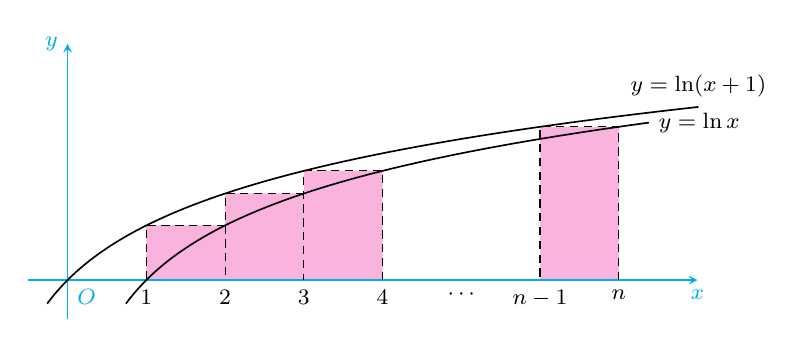
\begin{tikzpicture}[samples=100,>=stealth,domain=0:4,font=\footnotesize]
            \coordinate (xMin) at (-0.5,0);
            \coordinate (xMax) at (8,0);
            \coordinate (yMin) at (0,-0.5);
            \coordinate (yMax) at (0,3);
            \fill[magenta!30] (4,0)--(4,1.386)--(3,1.386)--(3,1.099)--(2,1.099)--(2,0.693)--(1,0.693)--(1,0)--cycle;
            \fill[magenta!30] (7,0)--(7,1.946)--(6,1.946)--(6,0)--cycle;
            \draw[->,cyan] (xMin)--(0,0) node [below right] {$O$}--(xMax) node[below] {$x$};
            \draw[->,cyan] (yMin)--(yMax) node [left] {$y$};
            \draw[semithick,domain=-0.3:2] plot({exp(\x)},\x) node[right] {$y=\ln x$};
            \draw[semithick,domain=-0.3:2.2] plot({exp(\x)-1},\x) node[above] {$y=\ln (x+1)$};
            \foreach \i in {1,...,4} {
            \coordinate[label=below:{$\i$}] (x\i) at (\i,0);
            }
            \node[below] at (5,0) {$\cdots$};
            \node[below] at (6,0) {$n-1$};
            \node[below] at (7,0) {$n$};
            \draw[densely dashed] (4,0)--(4,1.386)--(3,1.386)--(3,0);
            \draw[densely dashed] (3,1.099)--(2,1.099)--(2,0);
            \draw[densely dashed] (2,0.693)--(1,0.693)--(1,0);
            \draw[densely dashed] (7,0)--(7,1.946)--(6,1.946)--(6,0);
        \end{tikzpicture}
        \caption{}
    \end{figure}
    由图可知: $\displaystyle\int _{1}^{n}\ln x\dd x\leqslant \sum ^{n}_{k=1}\ln k\leqslant \int ^{n}_{1}\ln\left( 1+x\right) \dd x$
    则有 $$\displaystyle\dfrac{n\ln n-n+1}{n\ln n}\leqslant \dfrac{1}{n\ln n}\sum ^{n}_{k=1}\ln k\leqslant \dfrac{\left( n+1\right) \ln \left( n+1\right) -n}{n\ln n}$$
    又因为 $\displaystyle\lim _{n\to \infty }\dfrac{n\ln n-n+1}{n\ln n}=\lim _{n\to \infty }\dfrac{\left( n+1\right) \ln \left( n+1\right) -n}{n\ln n}=1$,
    因此有夹逼准则, 原式$=\e .$\\
    \textbf{法二: }(Stolz 定理+L'Hospital 法则) 同上得到和式: $\displaystyle\lim _{n\to \infty }\dfrac{\displaystyle\sum\limits ^{n}_{k=1}\ln k}{n\ln n}\xlongequal[]{\text{Stolz}}\lim _{n\to \infty }\dfrac{\ln n}{n\ln n-\left( n-1\right) \ln \left( n-1\right) }$
    下面考虑该极限值 $\displaystyle I=\lim _{n\to \infty }\dfrac{n\ln n-\left( n-1\right) \ln \left( n-1\right) }{\ln n}$, 由 Heine 定理将其连续化为函数极限:
    $$I'=\lim _{x\to +\infty }\dfrac{x\ln x-\left( x-1\right) \ln \left( x-1\right) }{x\ln x}$$
    \begin{flalign*}
        I'\xlongequal[]{L'}\lim_{x\to+\infty}\dfrac{\ln x+1-\ln \left( x-1\right) -1}{\dfrac{1}{x}}=\lim_{x\to+\infty}x\ln\frac{x}{x-1}=\lim_{x\to+\infty}x\left(\frac{x}{x-1}-1\right)=1\Rightarrow\text{原式=}\e .
    \end{flalign*}
\end{solution}

\begin{example}
    求 $\displaystyle\lim_{n\to\infty}\prod_{k=1}^{n-1}\left(\frac{2^k}{2^{k+1}-1}\right)^{\frac{1}{2^{n-k}}}.$
\end{example}
\begin{solution}
    取对数降低运算等级, 故
    \begin{flalign*}
        I & =\lim_{n\to\infty}\prod_{k=1}^{n-1}\left(\frac{2^k}{2^{k+1}-1}\right)^{\frac{1}{2^{n-k}}}=\exp\lim_{n\to\infty}\sum_{k=1}^{n-1}\frac{1}{2^{n-k}}\ln\frac{2^k}{2^{k+1}-1}                                                                                                \\
          & =\exp\lim_{n\to\infty}\frac{1}{2^{n-1}}\sum_{k=1}^{n-1}2^{k-1}\ln\frac{2^k}{2^{k+1}-1}\xlongequal[]{\text{Stolz}}\exp\lim_{n\to\infty}\frac{\left(\displaystyle\sum\limits_{k=1}^{n-1}-\sum\limits_{k=1}^{n-2}\right)2^{k-1}\ln\dfrac{2^k}{2^{k+1}}-1}{2^{n-1}-2^{n-2}} \\
          & =\exp\lim_{n\to\infty}\frac{2^{n-2}\ln\dfrac{2^{n-1}}{2^n-1}}{2^{n-1}-2^{n-2}}=\exp\lim_{n\to\infty}\ln\frac{1}{2-\dfrac{1}{2^{n-1}}}=\frac{1}{2}.
    \end{flalign*}
\end{solution}

\begin{example}
    求 $\displaystyle\lim_{n\to\infty}\frac{1}{n^2}\sum_{k=0}^{n}\ln\C _n^k.$
\end{example}
\begin{solution}
    Stolz 公式可重复使用,
    \begin{flalign*}
        \lim_{n\to\infty}S_n & \xlongequal[]{\text{Stolz}}\lim_{n\to\infty}\frac{\displaystyle\sum\limits_{k=0}^{n+1}\ln\C _{n+1}^k-\sum\limits_{k=0}^{n}\ln\C _{n}^k}{(n+1)^2-n^2}=\lim_{n\to\infty}\frac{\displaystyle\sum\limits_{k=0}^{n}\ln\dfrac{\C _{n+1}^k}{\C _n^k}+\ln\C _{n+1}^{n+1}}{2n+1} \\
                             & =\lim_{n\to\infty}\frac{\displaystyle\sum\limits_{k=0}^{n}\ln\dfrac{n+1}{n-k+1}}{2n+1}=\lim_{n\to\infty}\frac{\displaystyle(n+1)\ln(n+1)-\sum\limits_{k=1}^{n+1}\ln k}{2n+1}                                                                                            \\
                             & \xlongequal[]{\text{Stolz}}\lim_{n\to\infty}\frac{(n+1)\ln(n+1)-n\ln n-\ln(n+1)}{(2n+1)-(2n-1)}=\lim_{n\to\infty}\frac{\ln\left(\dfrac{n+1}{n}\right)^n}{2}=\frac{1}{2}.
    \end{flalign*}
\end{solution}

\begin{example}
    求极限 $\displaystyle\lim_{n\to\infty}\qty(\prod_{k=0}^{n}\C _n^k)^{\frac{2}{n(n+1)}}.$
\end{example}
\begin{solution}
    取对数, 降低运算等级, 有
    \begin{flalign*}
        I & =\exp\lim_{n\to\infty}\dfrac{2}{n(n+1)}\ln\prod_{k=0}^{\infty}\C_n^k=\exp\lim_{n\to\infty}\dfrac{\displaystyle 2\sum_{k=0}^{n}\ln\C_n^k}{n(n+1)}\xlongequal{\text{Stolz}}\exp\lim_{n\to\infty}\dfrac{\displaystyle2\sum_{k=0}^{n+1}\ln\C_{n+1}^k-2\sum_{k=0}^{n}\ln\C_n^k}{(n+1)(n+2)-n(n+1)} \\
          & =\exp\lim_{n\to\infty}\dfrac{\displaystyle\sum_{k=0}^{n}\ln\dfrac{n+1}{n-k+1}}{n+1}=\dots=\exp\lim_{n\to\infty}\ln\qty(\dfrac{n+1}{n})^n=\e.
    \end{flalign*}
\end{solution}

\begin{example}
    \scriptsize\linespread{0.8}
    求 $\displaystyle\lim _{n\to \infty }\sqrt[n^{2}] {\dfrac{n!\left( n-1\right) !\cdots 2!}{n^{n}\left( n-1\right) ^{n-1}\cdots 2^{2}}}.$
\end{example}
\begin{solution}
    \scriptsize\linespread{0.8}
    由例题 \ref{Stirling} 可知, $n!=\sqrt{2\pi n}n^{n}\e ^{-n+\frac{\theta _{n}}{12n}},0 <\theta _{n} <1$, 那么
    \begin{flalign*}
        \text{原式}  =\exp \lim _{n\to \infty }\dfrac{\displaystyle\sum\limits ^{n}_{k=2}\ln k!-\sum\limits ^{n}_{k=2}\ln k^{k}}{n^{2}}\xlongequal[]{\text{Stolz}}\exp \lim _{n\to \infty }\dfrac{\ln n!-\ln n^{n}}{2n-1}
        \xlongequal[]{\text{Stirling}}\exp \lim _{n\to \infty }\dfrac{\ln \left( \sqrt{2\pi n}\e ^{-n}+\dfrac{\theta _{n}}{12n}\right) }{2n-1}=\e ^{-\frac{1}{2}}.
    \end{flalign*}
\end{solution}
% \begin{inference}
%     Stirling 公式是一条用来取 $n!$ 近似值的数学公式, 其公式为: 
%     $$n!=\sqrt{2\pi n}n^n \e ^{-n+\frac{\theta_n}{12n}}\text{ 或 }\ln n!=\frac{1}{2}\ln(2\pi)+\left(n+\frac{1}{2}\right)\ln n-n+\frac{\theta_n}{12n}$$
%     其中 $0<\theta_n<1.$
% \end{inference}

\begin{example}\scriptsize\linespread{0.8}
    求极限 $\displaystyle\lim _{n\to \infty }n^{2}\left( \dfrac{\pi ^{2}}{6}-\sum ^{n}_{k=1}\dfrac{1}{k^{2}}-\dfrac{1}{n}\right) .$
\end{example}
\begin{solution}\scriptsize\linespread{0.8}
    记 $\displaystyle m=\dfrac{\pi ^{2}}{6}=\lim _{n\to \infty }\sum ^{n}_{k=1}\dfrac{1}{k^{2}}$,
    \begin{flalign*}
        \text{原式} & =\lim _{n\to \infty }\dfrac{\displaystyle m-\sum\limits ^{n}_{k=1}\dfrac{1}{k^{2}}-\dfrac{1}{n}}{\dfrac{1}{n^{2}}}\xlongequal[]{\text{Stolz}}\lim _{n\to \infty }\dfrac{\displaystyle m-\sum\limits ^{n}_{k=1}\dfrac{1}{k^{2}}-\dfrac{1}{n}-\left( m-\sum\limits ^{n-1}_{k=1}\dfrac{1}{k^{2}}-\dfrac{1}{n-1}\right) }{\dfrac{1}{n^{2}}-\dfrac{1}{\left( n-1\right) ^{2}}} \\
                    & =\lim _{n\to \infty }\dfrac{-\dfrac{1}{n^{2}}+\dfrac{1}{n-1}-\dfrac{1}{n}}{\dfrac{1}{n^{2}}-\dfrac{1}{\left( n-1\right) ^{2}}}=\lim _{n\to \infty }\dfrac{-\left( n-1\right) ^{2}+n^{2}\left( n-1\right) -n \left( n-1\right) ^{2}}{\left( n-1\right) ^{2}-n^{2}}=\lim _{n\to \infty }\dfrac{n-1}{1-2n}=-\dfrac{1}{2}.
    \end{flalign*}
\end{solution}

\begin{example}\scriptsize\linespread{0.8}
    $\{\C _n^k\}_{k=0}^n$ 为二项式系数, $A_n,G_n$ 分别表示它们的算术平均值和几何平均值,
    试证: $$\lim_{n\to\infty}\sqrt[n]{A_n}=2,\lim_{n\to\infty}\sqrt[n]{G_n}=\sqrt{\e }.$$
\end{example}
\begin{proof}[{\songti \textbf{证}}]\scriptsize\linespread{0.8}
    因为 $\displaystyle A_n=\frac{1}{n+1}\sum_{k=0}^{n}\C _n^k=\frac{2^n}{n+1},~G_n=\left(\prod_{k=0}^{n}\C _n^k\right)^{\frac{1}{n+1}}=\e ^{\frac{1}{n+1}\sum\limits_{k=0}^{n}\ln\C _n^k}$,
    所以
    $\displaystyle\lim_{n\to\infty}\sqrt[n]{A_n}=\lim_{n\to\infty}\sqrt[n]{\frac{2^n}{n+1}}=2$
    \begin{flalign*}
        \lim_{n\to\infty}\sqrt[n]{G_n} & =\exp\lim_{n\to\infty}\frac{\displaystyle\sum\limits_{k=0}^{n}\ln\C _n^k}{n(n+1)}\xlongequal[]{\text{Stolz}}\exp\lim_{n\to\infty}\frac{\displaystyle\sum\limits_{k=0}^{n}\ln\C _n^k-\sum\limits_{k=0}^{n-1}\ln\C _{n-1}^k}{2n}           \\
                                       & =\exp\lim_{n\to\infty}\frac{\displaystyle\sum\limits_{k=1}^{n-1}\ln\C _n^k-\sum\limits_{k=1}^{n-2}\ln\C _{n-1}^k}{2n}=\exp\lim_{n\to\infty}\frac{\displaystyle\sum\limits_{k=1}^{n-2}\ln\dfrac{\C _n^k}{\C _{n-1}^k}+\ln\C _n^{n-1}}{2n} \\
                                       & =\exp\lim_{n\to\infty}\frac{\displaystyle\sum\limits_{k=1}^{n-2}\ln\dfrac{n}{n-k}+\ln n}{2n}=\exp\lim_{n\to\infty}\frac{1}{2}\left(-\frac{1}{n}\sum_{k=1}^{n-1}\ln\frac{n-k}{n}\right)                                                   \\
                                       & =\exp\left[-\frac{1}{2}\int_{0}^{1}\ln(1-x)\dd x\right]=\sqrt{\e }.
    \end{flalign*}
\end{proof}

% \begin{example}
%     $a,b,c$ 为非负实数, 求 $\displaystyle\lim_{n\to\infty}\dfrac{1}{n^3}\sum_{i=1}^{n}\sum_{j=1}^{n}\dfrac{ij}{\sqrt{i^2+j^2+ai+bj+c}}.$
% \end{example}
% \begin{solution}
%     令 $\displaystyle y_{n}=\dfrac{1}{n^{3}}\sum ^{n}_{i=1}\sum ^{n}_{j=1}\dfrac{ij}{\sqrt{i^{2}+j^{2}}}$, 那么
%     \begin{flalign*}
%         
%     \end{flalign*}
% \end{solution}

\subsubsection{函数极限的情况}

Stolz 定理可推广到函数极限的情况.

\begin{theorem}[$\infty/\infty$ 型]
    若 $T>0$ 为常数, 且满足
    \begin{enumerate}[label=(\arabic{*})]
        \item $g(x+T)>g(x),~\forall x\geqslant a;$
        \item $g(x)\to+\infty~  (x\to+\infty)$, 且 $f,g$ 在 $[a,+\infty)$ 内闭有界;
        \item $\displaystyle\lim_{x\to+\infty}\frac{f(x+T)-f(x)}{g(x+T)-g(x)}=l.$
    \end{enumerate}
    则 $\displaystyle\lim_{x\to+\infty}\frac{f(x)}{g(x)}=l$, (其中 $l$ 为有限数, $+\infty$ 或 $-\infty$).
    \index{函数 Stolz 定理}
\end{theorem}
\begin{theorem}[$0/0$ 型]
    若 $T>0$ 为常数, 且
    \begin{enumerate}[label=(\arabic{*})]
        \item $0<g(x+T)<g(x),\forall x\geqslant a$;
        \item $\displaystyle\lim_{x\to+\infty}f=\lim_{x\to+\infty}g=0$;
        \item $\displaystyle\lim_{x\to+\infty}\frac{f(x+T)-f(x)}{g(x+T)-g(x)}=l.$
    \end{enumerate}
    则 $\displaystyle\lim_{x\to+\infty}\frac{f(x)}{g(x)}=l$, (其中 $l$ 为有限数, $+\infty$ 或 $-\infty$).
\end{theorem}

\begin{example}\scriptsize\linespread{0.8}
    设 $f$ 在 $[a,+\infty)$ 上有定义, 且内闭有界 (即 $\forall [\alpha,\beta]\subset(a,+\infty),f\text{ 在 }[\alpha,\beta]\text{ 上有界}$),
    $$\displaystyle\lim_{n\to\infty}\dfrac{f(x+1)-f(x)}{x^n}=l$$ 其中 $l$ 为有限数, $+\infty$ 或 $-\infty$, 证明: $\displaystyle\lim_{x\to+\infty}\dfrac{f(x)}{x^{n+1}}=\dfrac{l}{n+1}.$
\end{example}
\begin{solution}\scriptsize\linespread{0.8}
    运用函数的 Stolz 定理, 得
    \begin{flalign*}
        \lim _{x\to +\infty }\dfrac{f\left( x\right) }{x^{n+1}} & =\lim _{x\to +\infty }\dfrac{f\left( x+1\right) -f\left( x\right) }{\left( x+1\right) ^{n+1}-x^{n+1}}=\lim _{x\to +\infty }\dfrac{f\left( x+1\right) -f\left( x\right) }{\left( n+1\right) x^{n}+\dfrac{n\left( n+1\right) }{1\cdot 2}x^{n-1}+\cdots +1} \\
                                                                        & =\lim _{x\to +\infty }\dfrac{\dfrac{f\left( x+1\right) -f\left( x\right) }{x^{n}}}{\left( n+1\right) +\dfrac{n\left( n+1\right) }{1\cdot 2}\dfrac{1}{x}+\ldots +\dfrac{1}{x^{n}}}=\dfrac{l}{n+1}~
        (l \text{ 为}+\infty,-\infty\text{ 也成立}).
    \end{flalign*}
\end{solution}

\subsubsection{Stolz 的应用}

\begin{example}
    对于数列 $x_0=a,0<a<\dfrac{\pi}{2},x_n=\sin x_{n-1}~  (n=1,2,\cdots)$, 证明:
    $$\lim_{n\to\infty}x_n=0,~\lim_{n\to\infty}\sqrt{\frac{n}{3}}x_n=1.$$
\end{example}
\begin{proof}[{\songti \textbf{证}}]
    \begin{enumerate}[label=(\arabic{*})]
        \item 因为 $0<a<\dfrac{\pi}{2},~x_0=a$, 递推可知 $$0<x_n=\sin x_{n-1}<x_{n-1}<\dfrac{\pi}{2}~  (n=1,2,\cdots)$$
              $\{x_n\}$ 单调递减且有下界 $0$, $\lim\limits_{n\to\infty}x_n$ 存在. 记 $\displaystyle\lim_{n\to\infty}x_n=A$, 知 $A=\sin A\Rightarrow A=0$, $\displaystyle\lim_{n\to\infty}x_n=0.$
        \item 要证 $\displaystyle \lim_{n\to\infty}\sqrt{\frac{n}{3}}x_n=1$, 即证 $\displaystyle\lim_{n\to\infty}\frac{n}{\dfrac{1}{x_n^2}}=3$
              \begin{flalign*}
                  \lim _{n\to \infty }\dfrac{n}{\dfrac{1}{x_{n}^{2}}} & \xlongequal[]{\text{Stolz}}\lim _{n\to \infty }\dfrac{n-\left( n-1\right) }{\dfrac{1}{x_{n}^{2}}-\dfrac{1}{x_{n-1}^{2}}}=\lim _{n\to \infty }\dfrac{1}{\dfrac{1}{\sin ^{2}x_{n-1}}-\dfrac{1}{x_{n-1}^{2}}}=\lim _{n\to \infty }\dfrac{x_{n-1}^{2}\sin ^{2}x_{n}-1}{x_{n-1}^{2}-\sin ^{2}x_{n-1}} \\
                                                                              & =\lim _{x\to 0}\dfrac{x^{2}\sin ^{2}x}{x^{2}-\sin ^{2}x}=\lim _{x\to 0}\dfrac{x^{4}}{\left( x+\sin x\right) \left( x-\sin x\right) }=\lim _{x\to 0}\dfrac{x^{4}}{\left( 2x+o\left( x\right) \right) \left( \dfrac{x3}{6}+o\left( x^{3}\right) \right) }                                          \\
                                                                              & =\lim _{x\to 0}\dfrac{1}{\left( 2+o\left( 1\right) \right) \left( \dfrac{1}{6}+o\left( 1\right) \right) }=3.
              \end{flalign*}
              得证 $\displaystyle \lim_{n\to\infty}\sqrt{\frac{n}{3}}x_n=1.$
    \end{enumerate}
\end{proof}
\begin{example}
    设 $0<a_1<1,a_{n+1}=a_n(1-a_n)~  (\forall n\in\mathbb{N})$, 证明: $\displaystyle\lim_{n\to\infty}na_n=1.$
\end{example}
\begin{proof}[{\songti \textbf{证}}]
    由 $0<x_1<1$ 及 $x_2=x_1(1-x_1)$ 知,  $0<x_2<1$, 用数学归纳法可证: $\forall n\in\mathbb{N}^*:0<x_n<1$, 于是 $0<\dfrac{x_{n+1}}{x_{n}}=1-x_n<1~  (n=1,2,\cdots)$,
    从而 $\{x_n\}\searrow 0$, 不妨设 $\displaystyle\lim_{n\to\infty}x_n=A$, 递推关系式两边取极限, 得 $A=A(1-A)$, 解得 $A=0.$
    令 $b_n=\dfrac{1}{x_n}$, 则 $\displaystyle\lim_{n\to\infty}b_n=+\infty$, 且数列 $\{b_n\}$ 是严格单调递增, 故由 Stolz 定理
    $$\displaystyle\lim _{n\to \infty }nx_{n}=\lim _{n\to \infty }\dfrac{n}{\dfrac{1}{x_{n}}}=\lim _{n\to \infty }\dfrac{n}{b_{n}}=\lim _{n\to \infty }\dfrac{1}{b_{n+1}-b_{n}}=\lim _{n\to \infty }\left( 1-x_{n}\right) =1.$$
\end{proof}
\begin{example}
    设 $x_1>0,x_{n+1}=\ln(1+x_n)~  (n=1,2,\cdots)$, 求 $\lim\limits_{n\to\infty}nx_n.$
\end{example}
\begin{solution}
    $x_2=\ln(1+x_1)>0$, 用数学归纳法可证 $\forall n\in \mathbb{N}^*:x_n>0$, 又 $x_1>0,x_{n+1}=\ln(1+x_n)<x_n$, 故数列 $\{x_n\}\searrow 0$, 那么
    \begin{flalign*}
        \lim _{n\to \infty }nx_{n} & =\lim _{n\to \infty }\dfrac{n}{\dfrac{1}{x_{n}}}\xlongequal[]{\text{Stolz}}\lim _{n\to \infty }\dfrac{1}{\dfrac{1}{x_{n}}-\dfrac{1}{x_{n}-1}}=\lim _{n\to \infty }\dfrac{1}{\dfrac{1}{\ln \left( 1+x_{n-1}\right) }-\dfrac{1}{x_{n-1}}} \\
                                           & =\lim _{n\to \infty }\dfrac{x_{n-1}\ln \left( 1+x_{n-1}\right) }{x_{n-1}-\ln \left( 1+x_{n-1}\right) }=\lim _{n\to \infty }\dfrac{x_{n-1}^{2}}{\dfrac{1}{2}x_{n-1}^{2}}=2.
    \end{flalign*}
\end{solution}

\begin{example}
    设数列 $\qty{x_n}$ 满足 $x_n=\sin(x_{n-1})$, 其中 $n=1,2,3,\cdots$, 且满足 $x_0\in\qty(0,\dfrac{\pi}{2})$, 求极限 $\displaystyle \lim_{n \to +\infty}n\cdot x_n^2.$
\end{example}
\begin{solution}
    因为 $x_n=\sin(x_{n-1}),n=1,2, \cdots $, 且 $x_0\in\qty(0,\dfrac{\pi}{2})$, 由数学归纳法可知: $x_n>0,~(n=1,2, \cdots )$, 且 $x_n=\sin(x_{n-1})<x_{n-1}$, 所以, 数列 $\qty{x_n}$ 单调递减且有下界, 故数列 $\qty{x_n}$ 收敛, 设 $\displaystyle A=\lim_{n \to +\infty}x_{n}$, 在等式两边 $x_n=\sin(x_{n-1})$ 两边取极限可得
    $$
        \lim_{n \to +\infty}x_n=\lim_{n \to +\infty}\sin(x_{n-1})=\sin\qty(\lim_{n \to +\infty}x_{n-1})\Rightarrow A=0
    $$
    因此 $\displaystyle \lim_{n \to +\infty}\dfrac{1}{x_n^2}=+\infty$, 由 Stolz 定理可知,
    \begin{flalign*}
        \lim_{n\to+\infty}n\cdot x_n^2 & =\lim_{n\to+\infty}\dfrac{n}{\dfrac{1}{x_n^2}}=\lim_{n\to+\infty}\dfrac{n-(n-1)}{\dfrac{1}{x_n^2}-\dfrac{1}{x_{n-1}^2}}=\lim_{n\to+\infty}\dfrac{x_n^2 x_{n-1}^2}{\qty(x_{n-1}+x_n)\qty(x_{n-1}-x_n)} \\
                                       & =\lim_{n\to+\infty}\dfrac{x_{n-1}^{4}}{\qty(x_{n-1}+\sin\qty(x_{n-1}))\qty(x_{n-1}-\sin\qty(x_{n-1}))}=\lim_{n\to+\infty}\dfrac{x_{n-1}^{4}}{2x_{n-1}\cdot \dfrac{1}{6}x_{n-1}^{3}}=3.
    \end{flalign*}
\end{solution}

% \begin{example}
%     令 $a_n=1-\dfrac{\mathrm{C}_n^1}{3}+\dfrac{\mathrm{C}_n^2}{5}-\cdots+\dfrac{(-1)\mathrm{C}_n^n}{2n+1}$, 且 $\qty{b_n}_{n=2}^{\infty}$, 
%     且 $$b_n=\dfrac{(n+1)^2}{\sqrt[n+1]{(n+1)!}}-\dfrac{n^2}{\sqrt[n]{n!}}$$
%     计算极限 $\displaystyle\lim_{n\to\infty}\qty(1+\dfrac{\sqrt[n]{a_n}}{n!})^{\frac{n!}{b_n^n}}.$
% \end{example}
% \begin{solution}
%     因为 $\displaystyle a_n=\sum_{k=0}^{n}\dfrac{(-1)^k\mathrm{C}_n^k}{2k+1}=\int_{0}^{1}\qty[\sum_{k=0}^{n}\mathrm{C}_n^k\qty(-x^2)^k]\dd x=\int_{0}^{1}\qty(1-x^2)\dd x\xlongequal[]{x=\sin t}\int_{0}^{\frac{\pi}{2}}\cos^{2n+1}t\dd t$, 又由推论 \ref{Wallis gs} 可知, 
%     $$\int_{0}^{\frac{\pi}{2}}\cos^{2n+1}t\dd t=\dfrac{(2n)!!}{(2n+1)!!}\to0~ (n\to\infty)$$
% \end{solution}

\begin{example}\scriptsize\linespread{0.8}
    序列 $a_{ij}=\dfrac{i+j}{i^2+j^2}$, 求极限 $\displaystyle\lim_{n\to\infty}\dfrac{1}{n}\sum_{i=1}^{n}\sum_{j=1}^{n}a_{ij}.$
\end{example}
\begin{solution}\scriptsize\linespread{0.8}
    由 Stolz ($*/\infty$ 型) 得\footnote{以下的括号不为矩阵符号,
        \begin{flalign*}
             & \begin{pmatrix}
                          & \dfrac{1+1}{1^2+1^2}       & + & \dfrac{1+2}{1^2+2^2}       & + & \cdots & + & \dfrac{1+n}{1^2+n^2}       & + & \dfrac{1+n+1}{1^2+(n+1)^2}       \\
                   +      & \dfrac{2+1}{2^2+1^2}       & + & \dfrac{2+2}{2^2+2^2}       & + & \cdots & + & \dfrac{2+n}{2^2+n^2}       & + & \dfrac{2+n+1}{2^2+(n+1)^2}       \\
                   \vdots & \vdots                     &   & \vdots                     &   &        &   & \vdots                     &   & \vdots                           \\
                   +      & \dfrac{n+1}{n^2+1^2}       & + & \dfrac{n+2}{n^2+2^2}       & + & \cdots & + & \dfrac{n+n}{n^2+n^2}       & + & \dfrac{n+n+1}{n^2+(n+1)^2}       \\
                   +      & \dfrac{n+1+1}{(n+1)^2+1^2} & + & \dfrac{n+1+2}{(n+1)^2+2^2} & + & \cdots & + & \dfrac{n+1+n}{(n+1)^2+n^2} & + & \dfrac{n+1+n+1}{(n+1)^2+(n+1)^2}
               \end{pmatrix} \\
             & -
            \begin{pmatrix}
                       & \dfrac{1+1}{1^2+1^2} & + & \dfrac{1+2}{1^2+2^2} & + & \cdots & + & \dfrac{1+n}{1^2+n^2} \\
                +      & \dfrac{2+1}{2^2+1^2} & + & \dfrac{2+2}{2^2+2^2} & + & \cdots & + & \dfrac{2+n}{2^2+n^2} \\
                \vdots & \vdots               &   & \vdots               &   &        &   & \vdots               \\
                +      & \dfrac{n+1}{n^2+1^2} & + & \dfrac{n+2}{n^2+2^2} & + & \cdots & + & \dfrac{n+n}{n^2+n^2}
            \end{pmatrix}
            =2\left[ \sum ^{n}_{k=1}\dfrac{(n+1) +k}{(n+1) ^{2}+k^{2}}\right] +\dfrac{1}{n+1}.
        \end{flalign*}}
    \begin{flalign*}
        \lim _{n\to \infty }\dfrac{1}{n}\sum ^{n}_{i=1}\sum ^{n}_{j=1}\dfrac{i+j}{i^{2}+j^{2}} & =\lim _{n\to \infty }\left( \sum ^{n+1}_{i=1}\sum ^{n+1}_{j=1}-\sum ^{n}_{i=1}\sum ^{n}_{j=1}\right) \dfrac{i+j}{i^{2}+j^{2}}=\lim _{n\to \infty }\left[ 2\left( \sum ^{n}_{k=1}\dfrac{(n+1) +k}{(n+1) ^{2}+k^{2}}\right) +\dfrac{1}{n+1}\right] \\
                                                                                                       & =\lim _{n\to \infty }\left[ \dfrac{2}{n+1}\left( \sum ^{n}_{k=1}\dfrac{1+\dfrac{k}{n+1}}{1+\left( \dfrac{k}{n+1}\right) ^{2}}\right) +\dfrac{1}{n+1}\right] =2\int _{0}^{1}\dfrac{1+x}{1+x^{2}}\dd x=\dfrac{\pi}{2}+\ln 2.
    \end{flalign*}
\end{solution}

\begin{example}\scriptsize\linespread{0.8}
    序列 $a_{ij}=\dfrac{ij}{\sqrt{i^2+j^2+ai+bj+c}},~a,b,c$ 为非负实数, 求 $\displaystyle\lim_{n\to\infty}\dfrac{1}{n^3}\sum_{i=1}^{n}\sum_{j=1}^{n}a_{ij}.$
\end{example}
\begin{solution}\scriptsize\linespread{0.8}
    令 $\displaystyle y_{n}=\dfrac{1}{n^{3}}\sum\limits ^{n}_{i=1}\sum\limits ^{n}_{j=1}\dfrac{ij}{\sqrt{i^{2}+j^{2}}}$, 那么
    \begin{flalign*}
        \lim _{n\to \infty }y_{n} & \xlongequal[]{\text{Stolz}}\lim _{n\to \infty }\dfrac{\displaystyle\left( \sum\limits ^{n+1}_{i=1}\sum\limits ^{n+1}_{j=1}-\sum\limits ^{n}_{i=1}\sum\limits ^{n}_{j=1}\right) \dfrac{ij}{\sqrt{i^{2}+j^{2}}}}{3n^{2}+3n+1}=\lim _{n\to \infty }\dfrac{\displaystyle\left[ 2\left( \sum\limits ^{n}_{k=1}\dfrac{k(n+1) }{\sqrt{k^{2}+(n+1) ^{2}}}\right) +\dfrac{n+1}{\sqrt{2}}\right] }{3n^{2}+3n+1} \\
                                          & =\lim _{n\to \infty }\dfrac{2(n+1) ^{2}}{3n^{2}+3n+1}\cdot \lim _{n\to \infty }\dfrac{1}{n+1}\sum ^{n}_{k=1}\dfrac{k/(n+1) }{\sqrt{1+\left( k/(n+1) \right) ^{2}}}=\dfrac{2}{3}\int_{0}^{1}\dfrac{x}{\sqrt{1+x^2}}\dd x=\dfrac{2}{3}\left(\sqrt{2}-1\right).
    \end{flalign*}
    考虑 $\delta>0$ 的情况, 令 $\displaystyle z_{n}=\dfrac{1}{n^{3}}\sum ^{n}_{i=1}\sum ^{n}_{j=1}\dfrac{ij}{\sqrt{\left( i+\delta \right) ^{2}+\left( j+\delta \right) ^{2}}}$, 下证 $\displaystyle\lim _{n\to \infty }\left( z_{n}-y_{n}\right) =0$,
    \begin{flalign*}
        d_n=z_n-y_n=\dfrac{-1}{n^3}\sum ^{n}_{i=1}\sum ^{n}_{j=1}\dfrac{\left( 2\delta ^{2}+2\delta i+2\delta j\right) ij}{\sqrt{\left( i+\delta \right) ^{2}+\left( j+\delta \right) ^{2}}\sqrt{i^{2}+j^{2}}\left( \sqrt{\left( i+\delta \right) ^{2}+\left( j+\delta \right) ^{2}}+\sqrt{i^{2}+j^2}\right) }
    \end{flalign*}
    由 $\sqrt{i^2+j^2}\geqslant\sqrt{2ij}$, 因此
    \begin{flalign*}
        |d_n| & \leqslant \dfrac{1}{n^{3}}\sum ^{n}_{i=1}\sum ^{n}_{j=1}\dfrac{\left( 2\delta ^{2}+2\delta i+2\delta j\right) ij}{\left( i^{2}+j^{2}\right) ^{\frac{3}{2}}}\leqslant \dfrac{1}{\sqrt{2}n^{3}}\sum ^{n}_{i=1}\sum ^{n}_{j=1}\dfrac{\delta ^{2}+\delta i+\delta j}{\sqrt{i}\sqrt{j}} \\
              & =\frac{\delta^{2}}{\sqrt{2} n^{3}}\left(\sum_{i=1}^{n} \frac{1}{\sqrt{i}}\right)\left(\sum_{j=1}^{n} \frac{1}{\sqrt{j}}\right)+\frac{\delta}{\sqrt{2}}\left(\frac{1}{n} \sum_{j=1}^{n} \frac{1}{\sqrt{j}}\right)\left(\frac{1}{n^{2}} \sum_{i=1}^{n} \sqrt{i}\right)
        +\frac{\delta}{\sqrt{2}}\left(\frac{1}{n} \sum_{i=1}^{n} \frac{1}{\sqrt{i}}\right)\left(\frac{1}{n^{2}} \sum_{j=1}^{n} \sqrt{j}\right)
    \end{flalign*}
    当 $n\to\infty$ 时, 有
    $$\lim _{n \to \infty} \frac{1}{n} \sum_{j=1}^{n} \frac{1}{\sqrt{j}}=0 \text {, }  \lim _{n \to \infty} \frac{1}{n^{2}} \sum_{j=1}^{n} \sqrt{j}=0 $$
    于是 $\lim\limits_{n\to\infty}d_n=0$, 令 $\displaystyle x_n=\lim_{n\to\infty}\dfrac{1}{n^3}\sum_{i=1}^{n}\sum_{j=1}^{n}a_{ij}$, 且
    $\xi=\max\left\{\dfrac{a}{2},\dfrac{b}{2},\sqrt{\dfrac{c}{2}}\right\}$, 得
    $$i^{2}+j^{2} \leqslant i^{2}+j^{2}+a i+b j+c \leqslant(i+\xi)^{2}+(j+\xi)^{2}$$
    因此 $z_n\leqslant x_n\leqslant y_n$, 两边取极限, 由夹逼准则得 $\displaystyle\lim_{n\to\infty}\dfrac{1}{n^3}\sum_{i=1}^{n}\sum_{j=1}^{n}a_{ij}=\dfrac{2}{3}\left(\sqrt{2}-1\right).$
\end{solution}